\documentclass[a4paper,12pt]{report}

% Packages for supporting German language and umlauts
\usepackage[utf8]{inputenc}  % Use UTF-8 encoding
\usepackage[T1]{fontenc}     % Use T1 font encoding
\usepackage[ngerman]{babel}  % German language support
\usepackage{csquotes}        % Context-sensitive quotation marks

% Set page margins
\usepackage{geometry}
\geometry{
    top=2cm,
    bottom=2cm,
    left=2cm,
    right=2cm
}




% Package for including graphics
\usepackage{graphicx}
\graphicspath{{./images/}}

% Package for tables
\usepackage{adjustbox}
\usepackage{multirow}
\usepackage{tabularx}

% Packages for mathematics
\usepackage{amsmath}
\usepackage{amssymb}

% Packages for code listings
\usepackage{listings}
\usepackage{xcolor}
\usepackage{caption}

% Define custom colors for listings
\definecolor{backcolour}{rgb}{0.95,0.95,0.92}
\definecolor{codegreen}{rgb}{0,0.6,0}

% Custom style for listings
\lstdefinestyle{myStyle}{
    backgroundcolor=\color{backcolour},   
    commentstyle=\color{codegreen},
    keywordstyle=\color{blue}\bfseries,
    stringstyle=\color{orange},
    basicstyle=\ttfamily\footnotesize,
    breakatwhitespace=false,         
    breaklines=true,                 
    keepspaces=true,                 
    numbers=left,       
    numbersep=5pt,                  
    showspaces=false,                
    showstringspaces=false,
    showtabs=false,                  
    tabsize=2,
    morekeywords={true, false, null, y, n}
}

% Set the title for the listings list
\renewcommand{\lstlistlistingname}{Code Beispiele}

% Apply the custom style to all listings
\lstset{
    style=myStyle,
    captionpos=b, % Position der Beschriftung
    label=lst:example, % Beispielhaftes Label
    abovecaptionskip=0pt
}

% Package for creating and managing glossaries and acronyms
\usepackage[toc,acronym]{glossaries}
\loadglsentries{glossary}    % Load glossary entries
\loadglsentries{acronyms}    % Load acronym entries
\makeglossaries

% Package for hyperlinks with hidden link boxes
\usepackage[hidelinks]{hyperref}

% Package for citations with numeric style
\usepackage[backend=biber,style=numeric,sorting=none]{biblatex}
\addbibresource{references.bib}

% Package for TikZ graphics
\usepackage{tikz}
\usetikzlibrary{shapes.multipart, positioning, arrows.meta, matrix}

% Other useful packages
\usepackage{float}      % Improved interface for floating objects
\usepackage{pdfpages}   % Include PDF documents
\usepackage{lipsum}     % For placeholder text

% Suppress specific warnings from biblatex
\usepackage{silence}
\WarningsOff[biblatex]

% Configure superscript citations
\makeatletter
\renewcommand\@makefntext[1]{%
    \noindent\makebox[0pt][r]{\@makefnmark\ }#1}
\makeatother

% Add horizontal line above footnotes
\usepackage{etoolbox}
\patchcmd{\footnoterule}{\kern-3pt}{\kern-3pt}{}{}
\renewcommand{\footnoterule}{%
  \kern -3pt
  \hbox to \columnwidth{\color{black}\leaders\hrule height 0.4pt\hfill}%
  \kern 2.6pt
}

% Define new citation macro for footnotes
\newcommand{\myfootcite}[2]{\footnote{\citeauthor{#1} (\citeyear{#1}), #2}}

% Set paragraph formatting
\setlength{\parindent}{0pt}  % No indentation
\setlength{\parskip}{1em}    % Add space between paragraphs

% Global equation numbering by chapter
\numberwithin{equation}{chapter}

% Package for section formatting
\usepackage{titlesec}

% Format for chapters
\titleformat{\chapter}[hang]
{\normalfont\LARGE\bfseries}{\thechapter\ }{10pt}{\LARGE\bfseries}
\titlespacing*{\chapter}{0pt}{-20pt}{10pt}

% Format for unnumbered chapters (e.g., lists)
\titleformat{name=\chapter,numberless}[block]
{\normalfont\LARGE\bfseries}{}{10pt}{\LARGE\bfseries}
\titlespacing*{\chapter}{0pt}{-20pt}{10pt}

\begin{document}

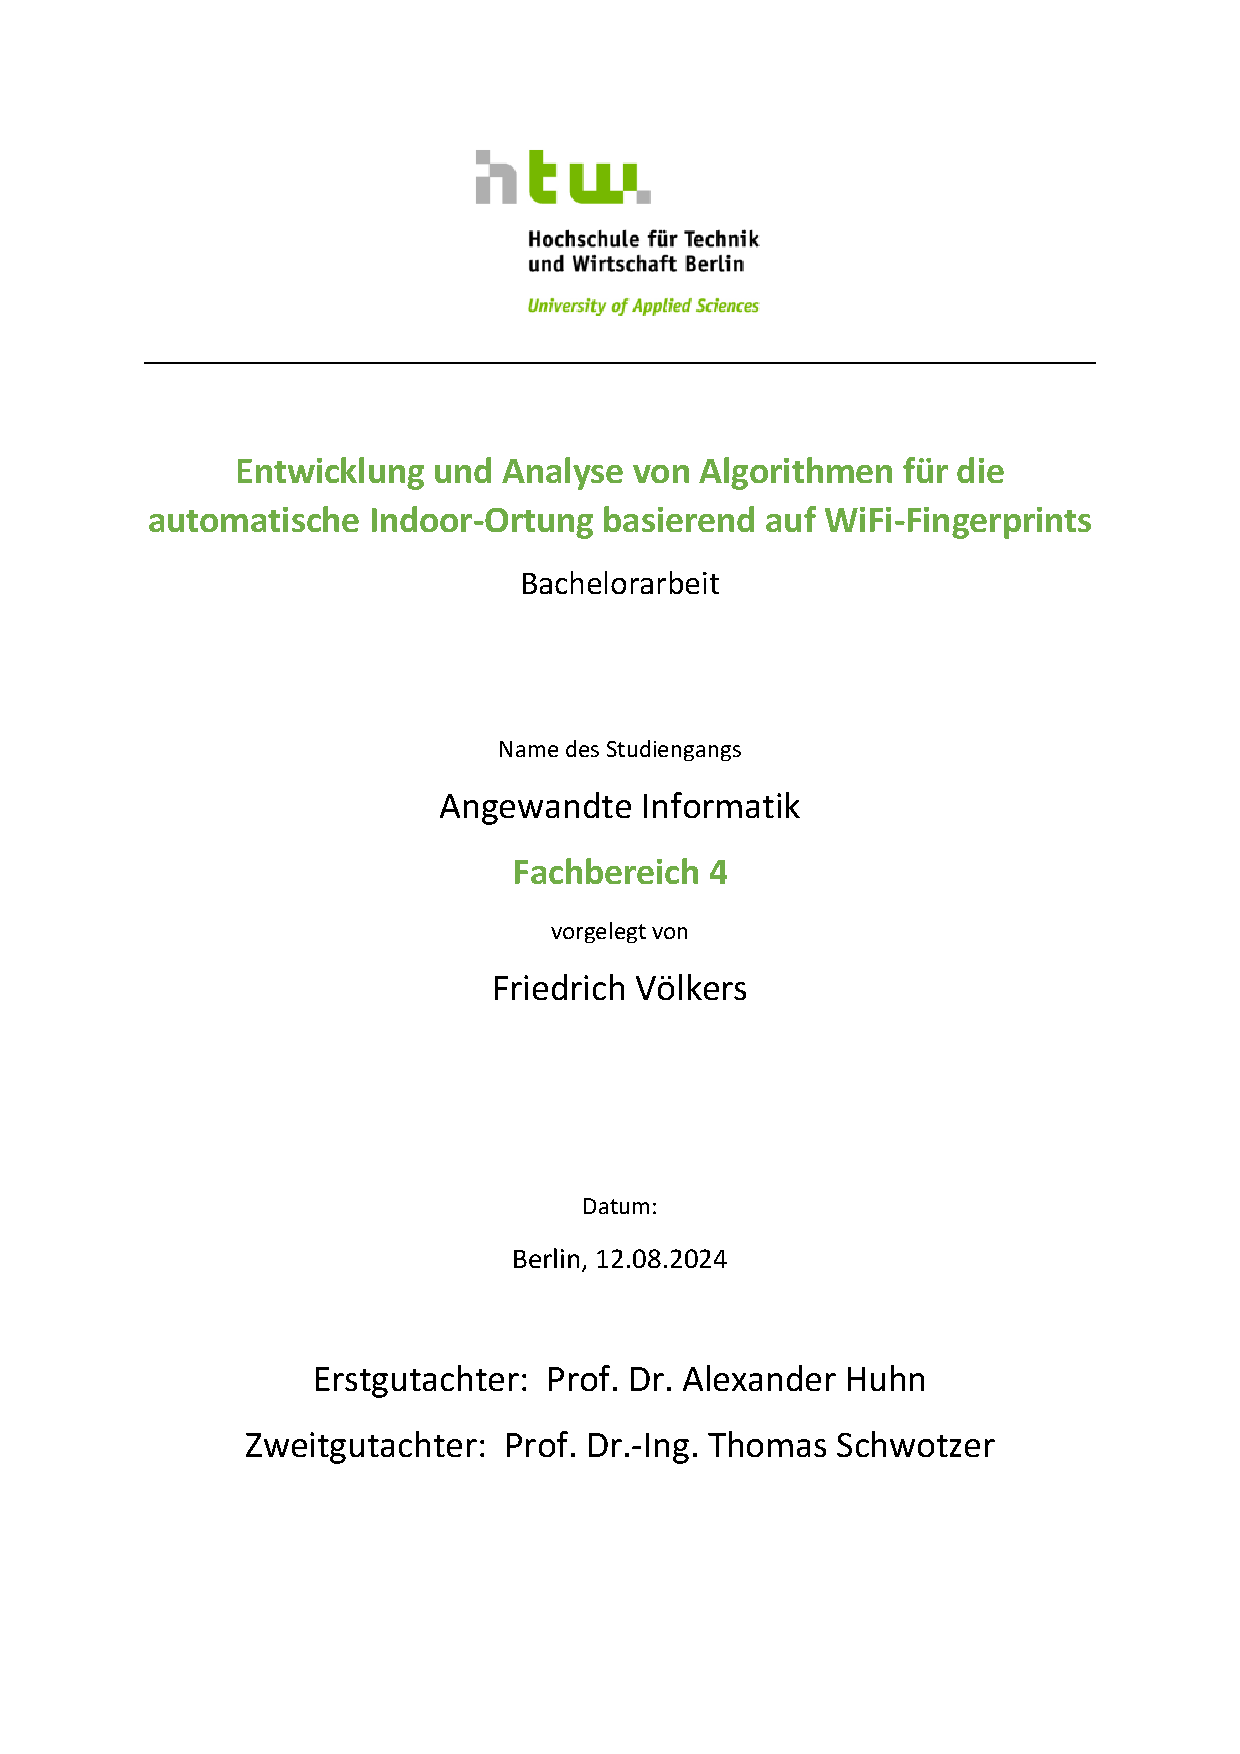
\includepdf[pages=1]{deckblatt.pdf}


% Title page without numbering
\pagenumbering{gobble}

% Title page
% \begin{titlepage}
%     \centering
%     \includegraphics[width=0.3\textwidth]{htw_logo.jpg}\par
%     \vspace*{1.6cm}
%     {\Huge\bfseries Entwicklung und Analyse von Algorithmen für die automatische Indoor-Ortung basierend auf WiFi-Fingerprints \par}
%     \vspace{1.5cm}
%     {\LARGE Bachelorarbeit \par}
%     \vspace{2cm}
%     {\Large\itshape Friedrich Völkers \par}
%     {\itshape 585012 \par}
%     \vfill
%     Betreuer: Prof. Dr. Alexander Huhn \\
%     Zweitbetreuer: Prof. Dr.-Ing. Thomas Schwotzer
%     \vspace{1cm}
%     \vfill
%     {\large \today\par}
% \end{titlepage}

% Directories with Roman numbering
\pagenumbering{Roman}

% Table of contents without numbering
\tableofcontents

% Verzeichnis der Listings
% \listofcodes

\begingroup
\setlength{\parskip}{1em} % Adjust the spacing for the list of listings
\lstlistoflistings
\endgroup


% List of figures without numbering
\listoffigures

% List of tables without numbering
\listoftables

% Main content with Arabic numbering
\clearpage
\pagenumbering{arabic}

% Including chapters




% \chapter{Einleitung}
\section{Motivation und Zielsetzung}
\section{Aufbau der Arbeit}

% \chapter{Grundlagen}

Quelle 1: Access Points Service Set Identifier (SSID) for Localization and Tracking
Quelle 2: RSSI-Based Indoor Localization With the Internet of Things
Quelle 3: Survey on Indoor localization System and Recent Advances of WIFI Fingerprinting Technique

\section{WiFi-Fingerprinting}

Gute Grundlagenquelle: Overview of WiFi fingerprinting-based indoor positioning -> Was ist Indoor Ortung, was gibt es für Möglichkeiten, Offline/Online Phase, was für Modelle gibt es?

\section{Indoor-Ortung: Offline- und Online-Phase}
\section{SSID, BSSID und RSSI}


\subsection{SSID}

Der Service Set Identifier (SSID) ist ein eindeutiger Bezeichner, der ein drahtloses Netzwerk kennzeichnet. SSIDs sind alphanumerische Zeichenfolgen, die vom Netzwerkadministrator festgelegt werden. Die SSID ermöglicht es Nutzern, zwischen verschiedenen WiFi-Netzwerken zu unterscheiden und das gewünschte Netzwerk auszuwählen. In einem Indoor-Lokalisierungsszenario kann die SSID als Landmarke für Access Points genutzt werden, um die Position eines Benutzers zu bestimmen (Quelle 1, Kapitel 1, Seite 5460).

\subsection{BSSID}

Der Basic Service Set Identifier (BSSID) ist eine eindeutige Kennung für jeden Access Point innerhalb eines WiFi-Netzwerks. Diese Kennung besteht aus der MAC-Adresse des Access Points, die fest zugewiesen und unveränderlich ist. In Netzwerken mit mehreren Access Points, die dieselbe SSID nutzen, ermöglicht die BSSID die genaue Unterscheidung der einzelnen Access Points. Dies ist besonders wichtig für die Lokalisierung und Netzwerkverwaltung, da es die Identifikation und Verfolgung spezifischer Access Points ermöglicht (Quelle 1, Kapitel 1, Seite 5460).

\subsection{RSSI}

Der Received Signal Strength Indicator (RSSI) ist ein Maß für die Stärke des empfangenen WiFi-Signals an einem bestimmten Punkt. RSSI-Werte werden von der Netzwerkkarte des Geräts gemessen und in der App aufgezeichnet. Diese Werte spielen eine entscheidende Rolle bei der Erstellung von Fingerprints für die Indoor-Lokalisierung, da die Signalstärke als Indikator für die Entfernung zwischen dem Gerät und dem Access Point genutzt wird. Schwächere RSSI-Werte deuten dabei auf eine größere Entfernung hin (Quelle 1, Kapitel 1, Seite 5464).

\section{Verhalten von RSSI-Werten in Bezug auf Entfernung}

Quelle 2:

Die RSSI-Werte nehmen mit zunehmender Distanz zwischen Sender und Empfänger ab, und können mit dem Pfadverlustmodell beschrieben werden. Das Pfadverlustmodell beschreibt den Zusammenhang zwischen der Entfernung und der Signalstärke, und wird durch die folgende Gleichung dargestellt:

\begin{equation}
    RSSI = -10n \log_{10}(d) + C
\end{equation}

wobei n der Pfadverlustexponent ist, der je nach Umgebung variiert, d die Distanz zwischen Sender und Empfänger ist und A der RSSI-Wert in einem Meter Entfernung vom Sender ist.

Umgebung der Quelle: Im Raum sind viele Computer und eine große Anzahl an WiFi- und BLE-Geräten, Ein Forschungslabor mit den Abmessungen 10,8 m x 7,3 m.

Ergebnisse: n = 2.013, C = -49,99 dBm

Die Path-Loss-Modell-Gleichung mit den Parametern \(n = 2.013\) und \(C = -49.99\) ist:

In Abbildung \ref{fig:rssi_distance} ist der Zusammenhang zwischen RSSI und Entfernung dargestellt. Dieser Abschnitt dient dazu um eine Vorstellung davon zu bekommen, wie sich RSSI-Werte in Bezug auf die Entfernung verhalten.

\begin{figure}[h]
    \centering
    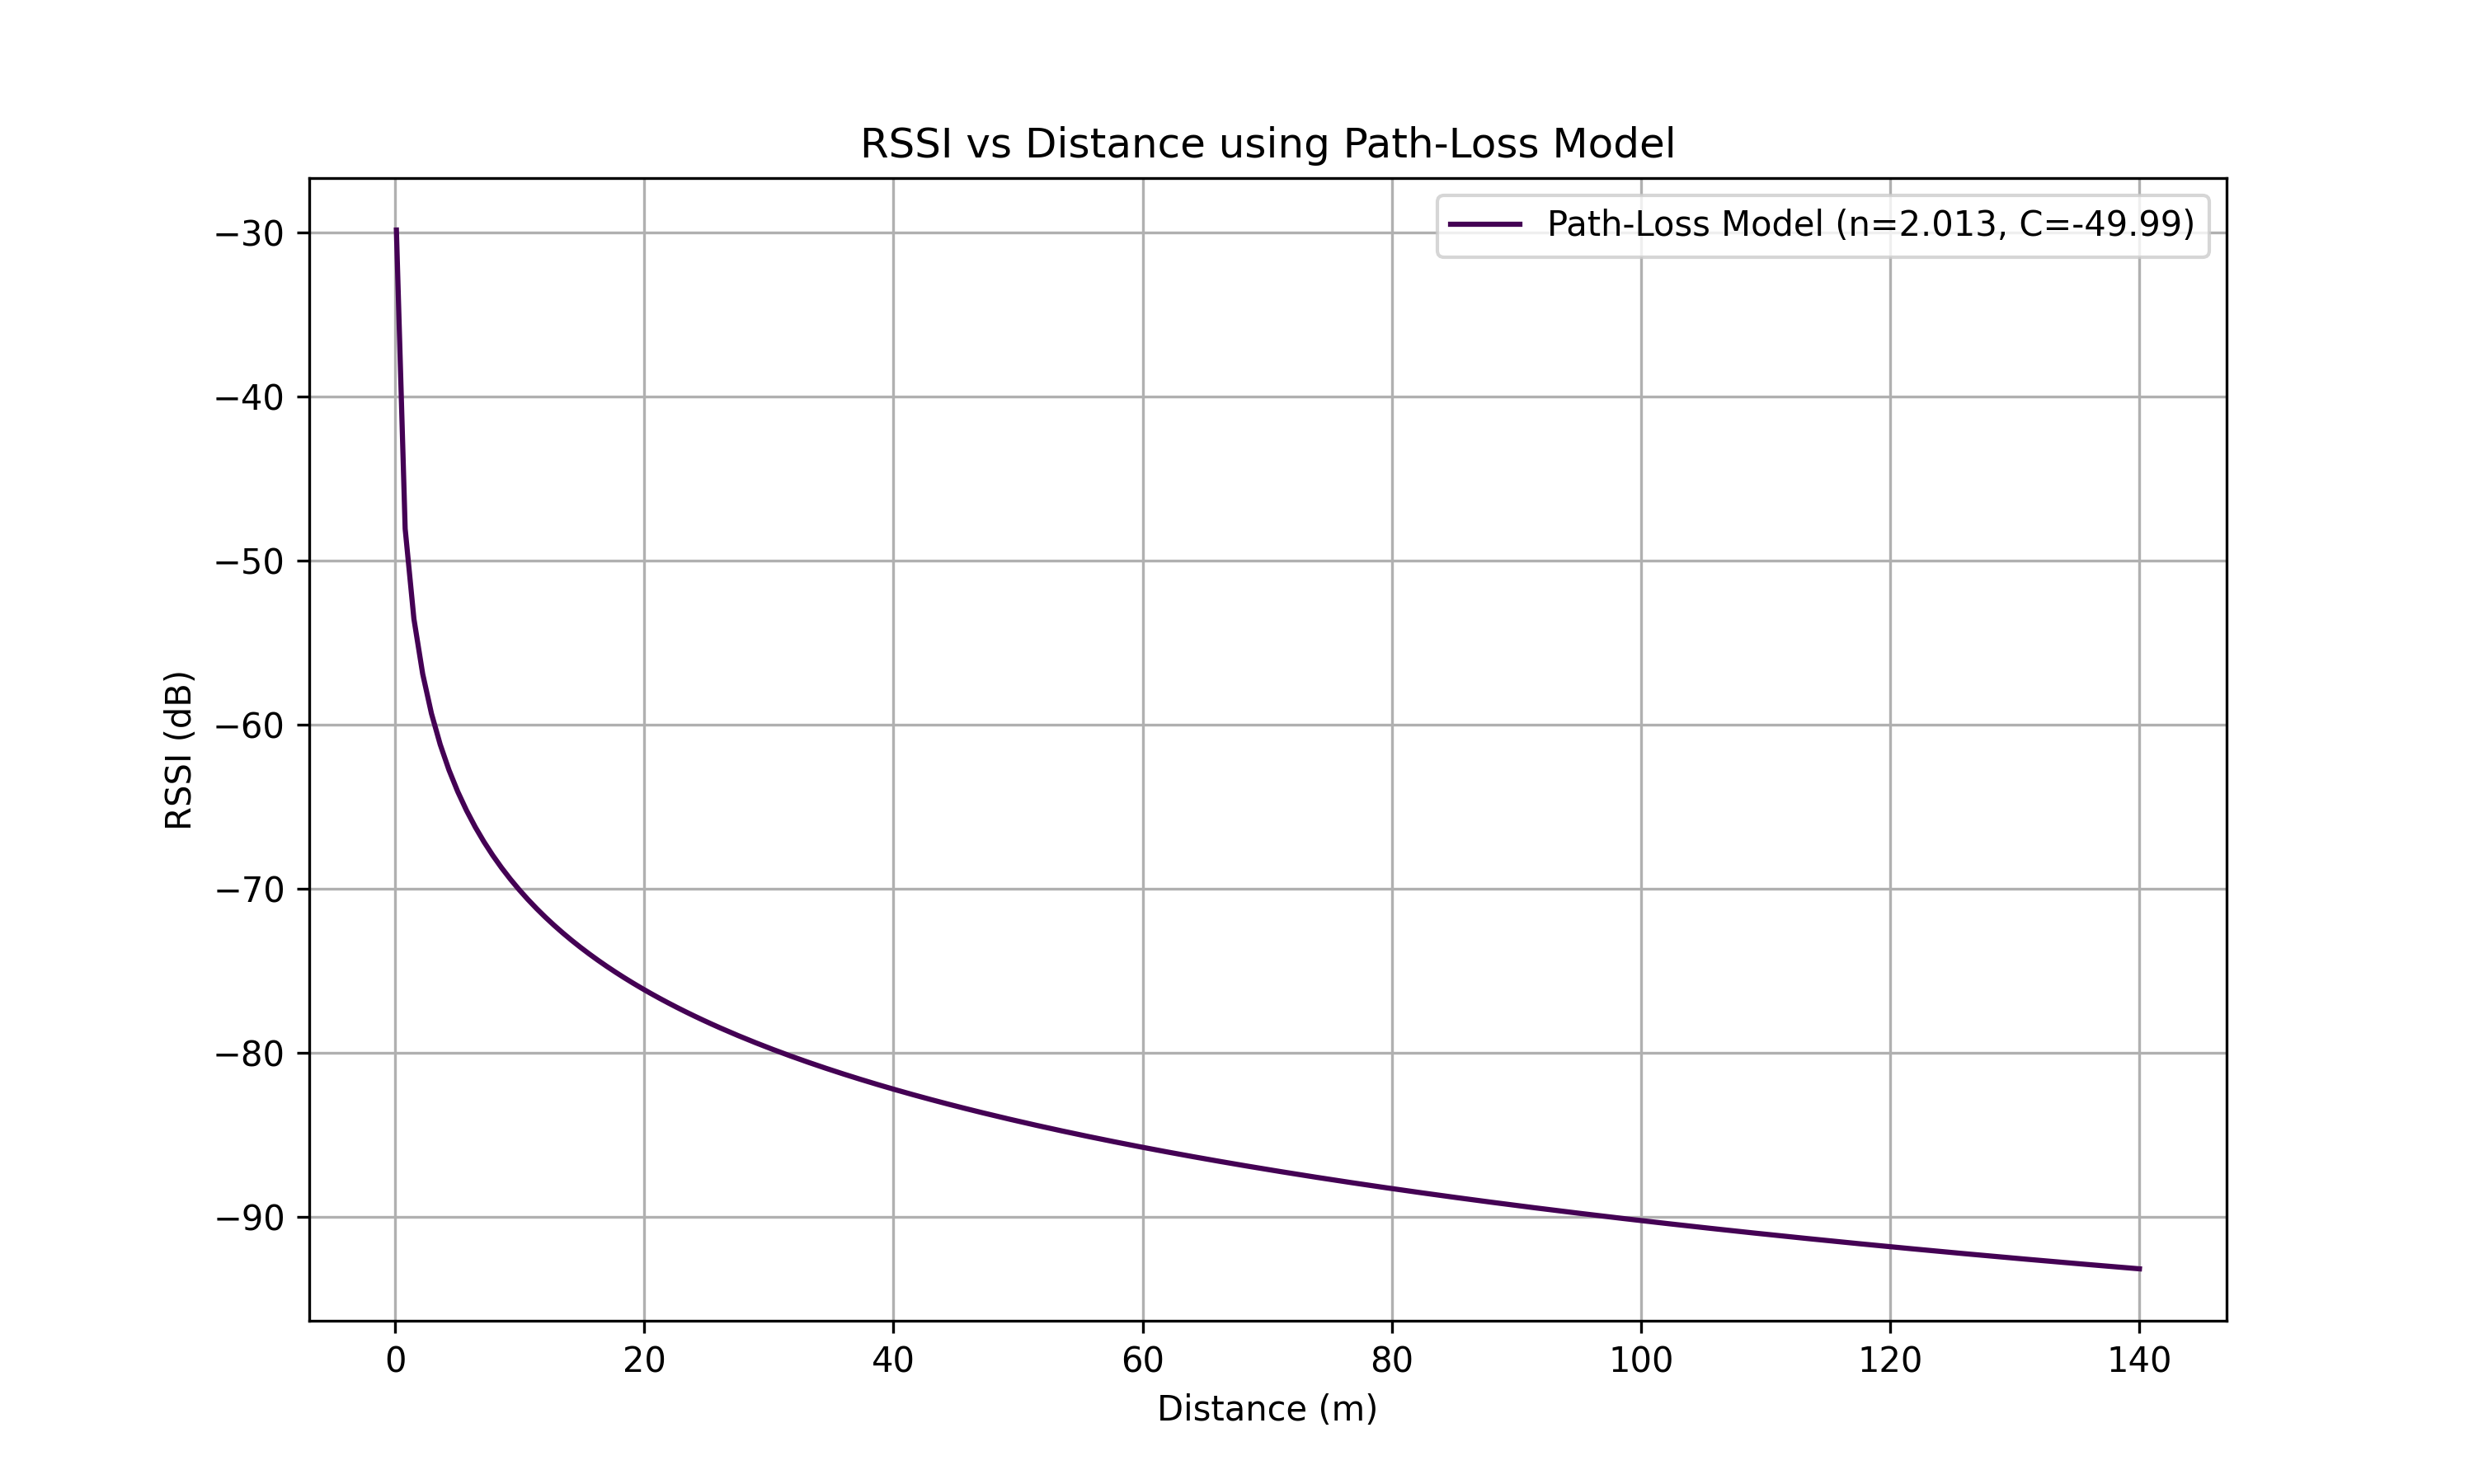
\includegraphics[width=0.8\textwidth]{images/rssi_distance.png}
    \caption{RSSI vs. Distance}
    \label{fig:rssi_distance}
\end{figure}
% \input{chapters/03_systemarchitektur}
% \input{chapters/04_implementierungsdetails}
% \input{chapters/05_datenerfassung_aufbereitung}
% \input{chapters/06_vergleich_algorithmen}
% \input{chapters/07_erweiterte_untersuchungen}
% \input{chapters/08_ergebnisse_diskussion}
% \input{chapters/09_fazit_ausblick}


\chapter{Einleitung}
\section{Motivation und Zielsetzung}
\section{Aufbau der Arbeit}

\chapter{Grundlagen}

Quelle 1: Access Points Service Set Identifier (SSID) for Localization and Tracking
Quelle 2: RSSI-Based Indoor Localization With the Internet of Things
Quelle 3: Survey on Indoor localization System and Recent Advances of WIFI Fingerprinting Technique

\section{WiFi-Fingerprinting}

Gute Grundlagenquelle: Overview of WiFi fingerprinting-based indoor positioning -> Was ist Indoor Ortung, was gibt es für Möglichkeiten, Offline/Online Phase, was für Modelle gibt es?

\section{Indoor-Ortung: Offline- und Online-Phase}
\section{SSID, BSSID und RSSI}


\subsection{SSID}

Der Service Set Identifier (SSID) ist ein eindeutiger Bezeichner, der ein drahtloses Netzwerk kennzeichnet. SSIDs sind alphanumerische Zeichenfolgen, die vom Netzwerkadministrator festgelegt werden. Die SSID ermöglicht es Nutzern, zwischen verschiedenen WiFi-Netzwerken zu unterscheiden und das gewünschte Netzwerk auszuwählen. In einem Indoor-Lokalisierungsszenario kann die SSID als Landmarke für Access Points genutzt werden, um die Position eines Benutzers zu bestimmen (Quelle 1, Kapitel 1, Seite 5460).

\subsection{BSSID}

Der Basic Service Set Identifier (BSSID) ist eine eindeutige Kennung für jeden Access Point innerhalb eines WiFi-Netzwerks. Diese Kennung besteht aus der MAC-Adresse des Access Points, die fest zugewiesen und unveränderlich ist. In Netzwerken mit mehreren Access Points, die dieselbe SSID nutzen, ermöglicht die BSSID die genaue Unterscheidung der einzelnen Access Points. Dies ist besonders wichtig für die Lokalisierung und Netzwerkverwaltung, da es die Identifikation und Verfolgung spezifischer Access Points ermöglicht (Quelle 1, Kapitel 1, Seite 5460).

\subsection{RSSI}

Der Received Signal Strength Indicator (RSSI) ist ein Maß für die Stärke des empfangenen WiFi-Signals an einem bestimmten Punkt. RSSI-Werte werden von der Netzwerkkarte des Geräts gemessen und in der App aufgezeichnet. Diese Werte spielen eine entscheidende Rolle bei der Erstellung von Fingerprints für die Indoor-Lokalisierung, da die Signalstärke als Indikator für die Entfernung zwischen dem Gerät und dem Access Point genutzt wird. Schwächere RSSI-Werte deuten dabei auf eine größere Entfernung hin (Quelle 1, Kapitel 1, Seite 5464).

\section{Verhalten von RSSI-Werten in Bezug auf Entfernung}

Quelle 2:

Die RSSI-Werte nehmen mit zunehmender Distanz zwischen Sender und Empfänger ab, und können mit dem Pfadverlustmodell beschrieben werden. Das Pfadverlustmodell beschreibt den Zusammenhang zwischen der Entfernung und der Signalstärke, und wird durch die folgende Gleichung dargestellt:

\begin{equation}
    RSSI = -10n \log_{10}(d) + C
\end{equation}

wobei n der Pfadverlustexponent ist, der je nach Umgebung variiert, d die Distanz zwischen Sender und Empfänger ist und A der RSSI-Wert in einem Meter Entfernung vom Sender ist.

Umgebung der Quelle: Im Raum sind viele Computer und eine große Anzahl an WiFi- und BLE-Geräten, Ein Forschungslabor mit den Abmessungen 10,8 m x 7,3 m.

Ergebnisse: n = 2.013, C = -49,99 dBm

Die Path-Loss-Modell-Gleichung mit den Parametern \(n = 2.013\) und \(C = -49.99\) ist:

In Abbildung \ref{fig:rssi_distance} ist der Zusammenhang zwischen RSSI und Entfernung dargestellt. Dieser Abschnitt dient dazu um eine Vorstellung davon zu bekommen, wie sich RSSI-Werte in Bezug auf die Entfernung verhalten.

\begin{figure}[h]
    \centering
    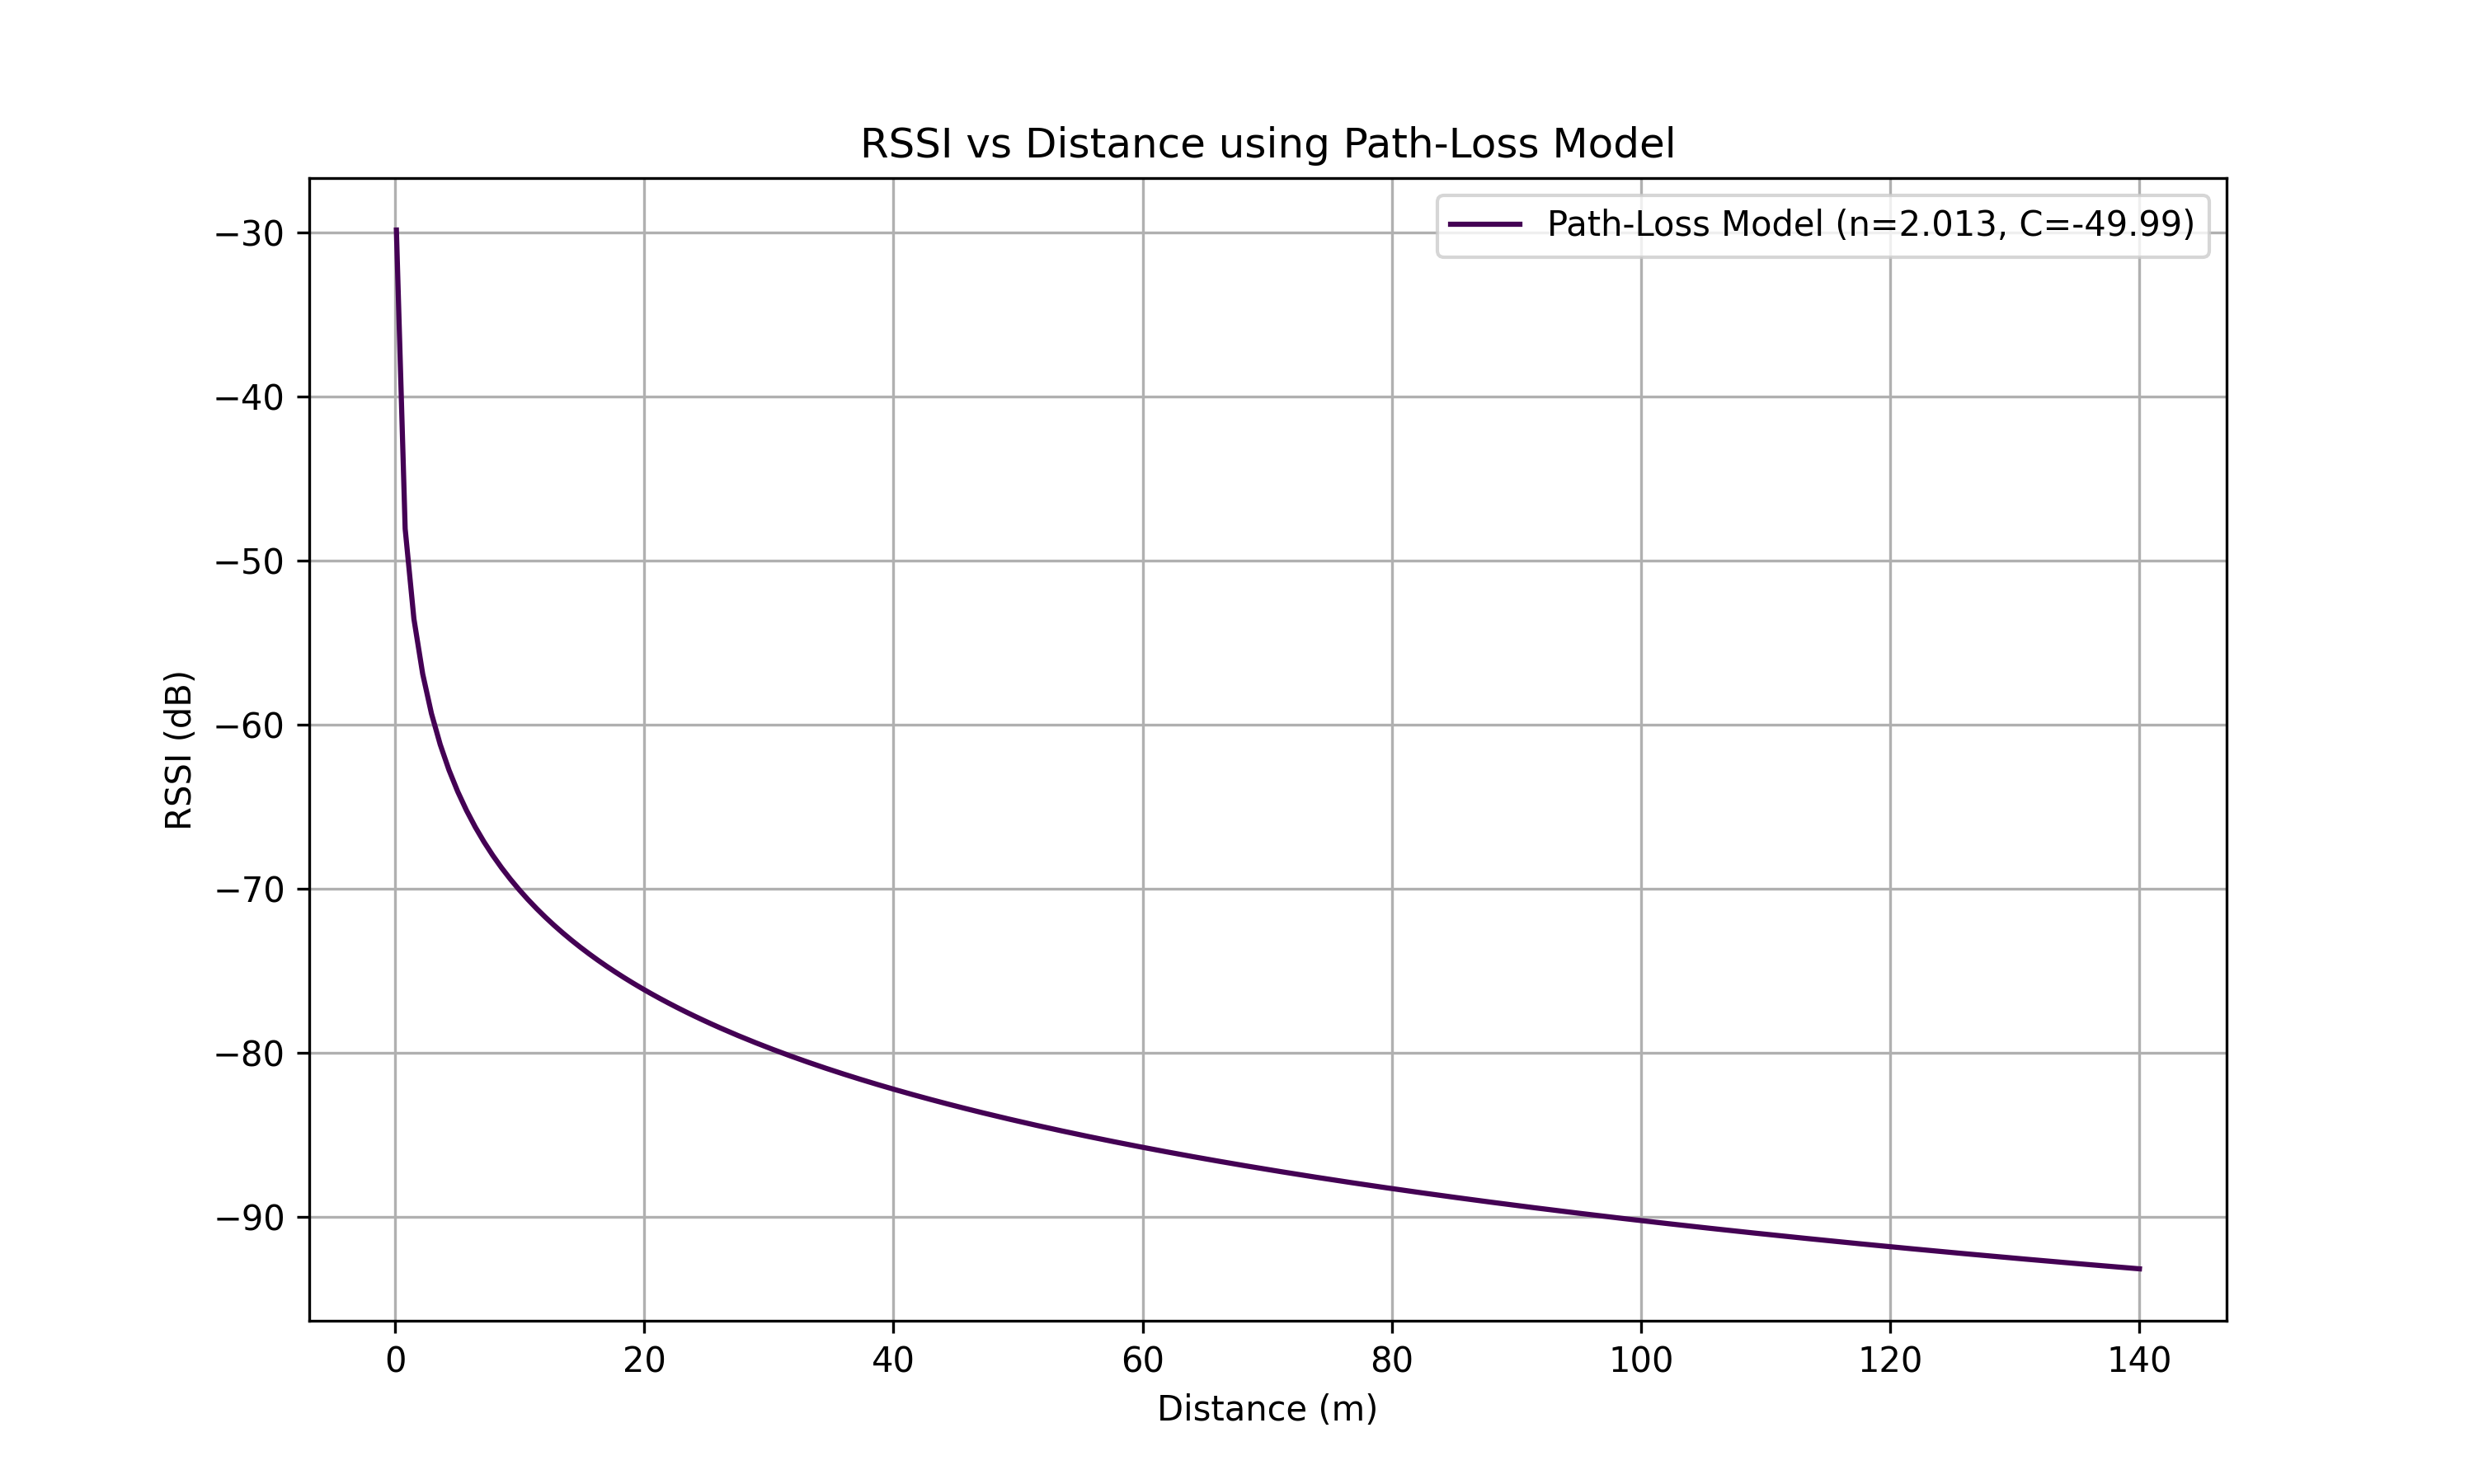
\includegraphics[width=0.8\textwidth]{images/rssi_distance.png}
    \caption{RSSI vs. Distance}
    \label{fig:rssi_distance}
\end{figure}
\chapter{Algorithmen und Methoden}

\begin{table}[h]
    \centering
    \begin{tabularx}{\textwidth}{|X|X|X|X|X|}
        \hline
        Router & Raum 1      & Raum 2      & Raum 3     & Unbekannt (1) \\ \hline
        1      & -73.67 dBm  & -91.12 dBm  & -69.37 dBm & -73.51 dBm    \\ \hline
        2      & -104.99 dBm & -64.47 dBm  & -89.65 dBm & -103.41 dBm   \\ \hline
        3      & -67.03 dBm  & -105.38 dBm & -88.40 dBm & -70.35 dBm    \\ \hline
    \end{tabularx}
    \caption{RSSI-Werte für die drei Router und die Räume}
    \label{tab:rssi_values}
\end{table}

\paragraph{Quellen für Auswahl}

\begin{itemize}
    \item https://ar5iv.labs.arxiv.org/html/2111.14281 -> KNN, SVM
    \item A Wireless Fingerprint Location Method Based on Target Tracking (Kapitel 3, Seite 3) -> KNN, SVM, Random Forest
    \item https://onlinelibrary.wiley.com/doi/full/10.1155/2017/6268797 -> KNN, SVM, Random Forest. In Table 2 stehen die Genauigkeiten der Algorithmen
\end{itemize}

\section{K-Nearest Neighbors (KNN)}
\textbf{Quellen:} \\
\href{https://www.ibm.com/de-de/topics/knn}{Quelle 1: https://www.ibm.com/de-de/topics/knn} \\
Quelle 4: Comprehensive analysis of distance and similarity measures for Wi-Fi fingerprinting indoor positioning systems \\
Quelle 5: Hechenbichler, Schliep: - Weighted k-Nearest-Neighbor Techniques and Ordinal Classification

\subsection{Algorithmusbeschreibung}
\textbf{Quelle 1:} Der k-nearest neighbor (KNN) Algorithmus ist ein überwachter Lernklassifikator, der auf dem Konzept der Nähe basiert und zur Lösung von Klassifikations- und Regressionsproblemen verwendet werden kann. Der Algorithmus funktioniert so, dass ein Datenpunkt mit den vorhandenen Datenpunkten in den Trainingsdaten verglichen wird und die Distanz zu jedem Datenpunkt berechnet wird. Basierend auf diesen Distanzen werden die k Datenpunkte ausgewählt, die den kleinsten Abstand haben. Aus diesen k Datenpunkten wird dann die Klasse bestimmt, die am häufigsten vertreten ist. Hierbei reicht bereits eine relative Mehrheit aus (wenn z.B. 4 Klassen vertreten sind, kann ein Anteil von mehr als 25 \% ausreichend sein).

\subsection{Distanzmetriken (euklidisch, Sorensen)}
\textbf{Quelle 1:} Für die Berechnung der Distanzen können verschiedene Distanzmetriken verwendet werden. Die am häufigsten verwendete Distanzmetrik ist der euklidische Abstand. In dieser Arbeit wurde entschieden, sowohl die euklidische Distanz als auch die Sorensen-Distanz zu verwenden. Bei der euklidischen Distanz wird das Quadrat der Abstände (Betrag der Differenz) zwischen zwei Werten gebildet, über alle Wertepaare aufsummiert und abschließend die Quadratwurzel dieser Summe gezogen (siehe \ref{eq:euclidean}).

\begin{equation}
    \label{eq:euclidean}
    \text{distance}_{\text{euclidean}}(P, Q) = \sqrt{\sum_{i=1}^{d} (P_i - Q_i)^2}
\end{equation}

\textbf{Quelle 4:} Bei der Sorensen-Distanzfunktion werden die Abstände der Datenpunkte aufsummiert und durch die Summe der Wertepaare zweier Datenpunkte geteilt (siehe \ref{eq:sorensen}). Grund für die Wahl dieser beiden Metriken: Die Arbeit "Comprehensive analysis of distance and similarity measures for Wi-Fi fingerprinting indoor positioning systems" konnte damit gute Ergebnisse erzielen. Der euklidische Abstand ist weit verbreitet und entspricht auch der bisherigen Implementierung in der App.

\begin{equation}
    \label{eq:sorensen}
    \text{distance}_{\text{sorensen}}(P, Q) = \frac{\sum_{i=1}^{d} |P_i - Q_i|}{\sum_{i=1}^{d} (P_i + Q_i)}
\end{equation}

In Abbildung \ref{fig:distance_metrics_heatmaps} sind die Heatmaps für die beiden Distanzmetriken dargestellt.

Damit die Unterschiede zwischen den beiden Distanzmetriken besser sichtbar sind, wurden die Distanzen zwischen allen möglichen Wertepaaren zwischen 0 und -100 berechnet und in Abbildung \ref{fig:distance_metrics_heatmaps} dargestellt. Wie zu erkennen ist, sind diese beiden symmetrisch zu der Geraden zwischen den beiden Punkten (0, 0) und (-100, -100). Wie zu erkennen ist, sind die Werte für die euklidische Distanz auch symmetrisch zu der Geraden zwischen den beiden Punkten (0, -100) und (-100, 0). Dementsprechend ist die Distanz alleine von der Differenz der beiden Werte abhängig. Bei der Sørensen-Distanz muss bei kleineren Werten der Abstand größer sein, um die gleiche Distanz zu erreichen wie bei kleineren Werten.

Um dies zu verdeutlichen, betrachten wir die Berechnung der Distanzen für zwei Beispielwertepaare:

Gegeben:
\begin{itemize}
    \item Wertepaar 1: \( P = -30 \, \text{dBm} \), \( Q = -40 \, \text{dBm} \)
    \item Wertepaar 2: \( P = -70 \, \text{dBm} \), \( Q = -80 \, \text{dBm} \)
\end{itemize}

\begin{table}[H]
    \centering
    \begin{tabular}{|c|c|c|}
        \hline
        Wertepaar                                & Sørensen-Dice Distanz & Euklidische Distanz \\
        \hline
        \(-30 \, \text{dBm}, -40 \, \text{dBm}\) & \(-0.142857\)         & \(10\)              \\
        \(-70 \, \text{dBm}, -80 \, \text{dBm}\) & \(-0.066667\)         & \(10\)              \\
        \hline
    \end{tabular}
    \caption{Berechnete Distanzen für die gegebenen Wertepaare}
    \label{tab:distance_results}
\end{table}

\begin{figure}[H]
    \centering
    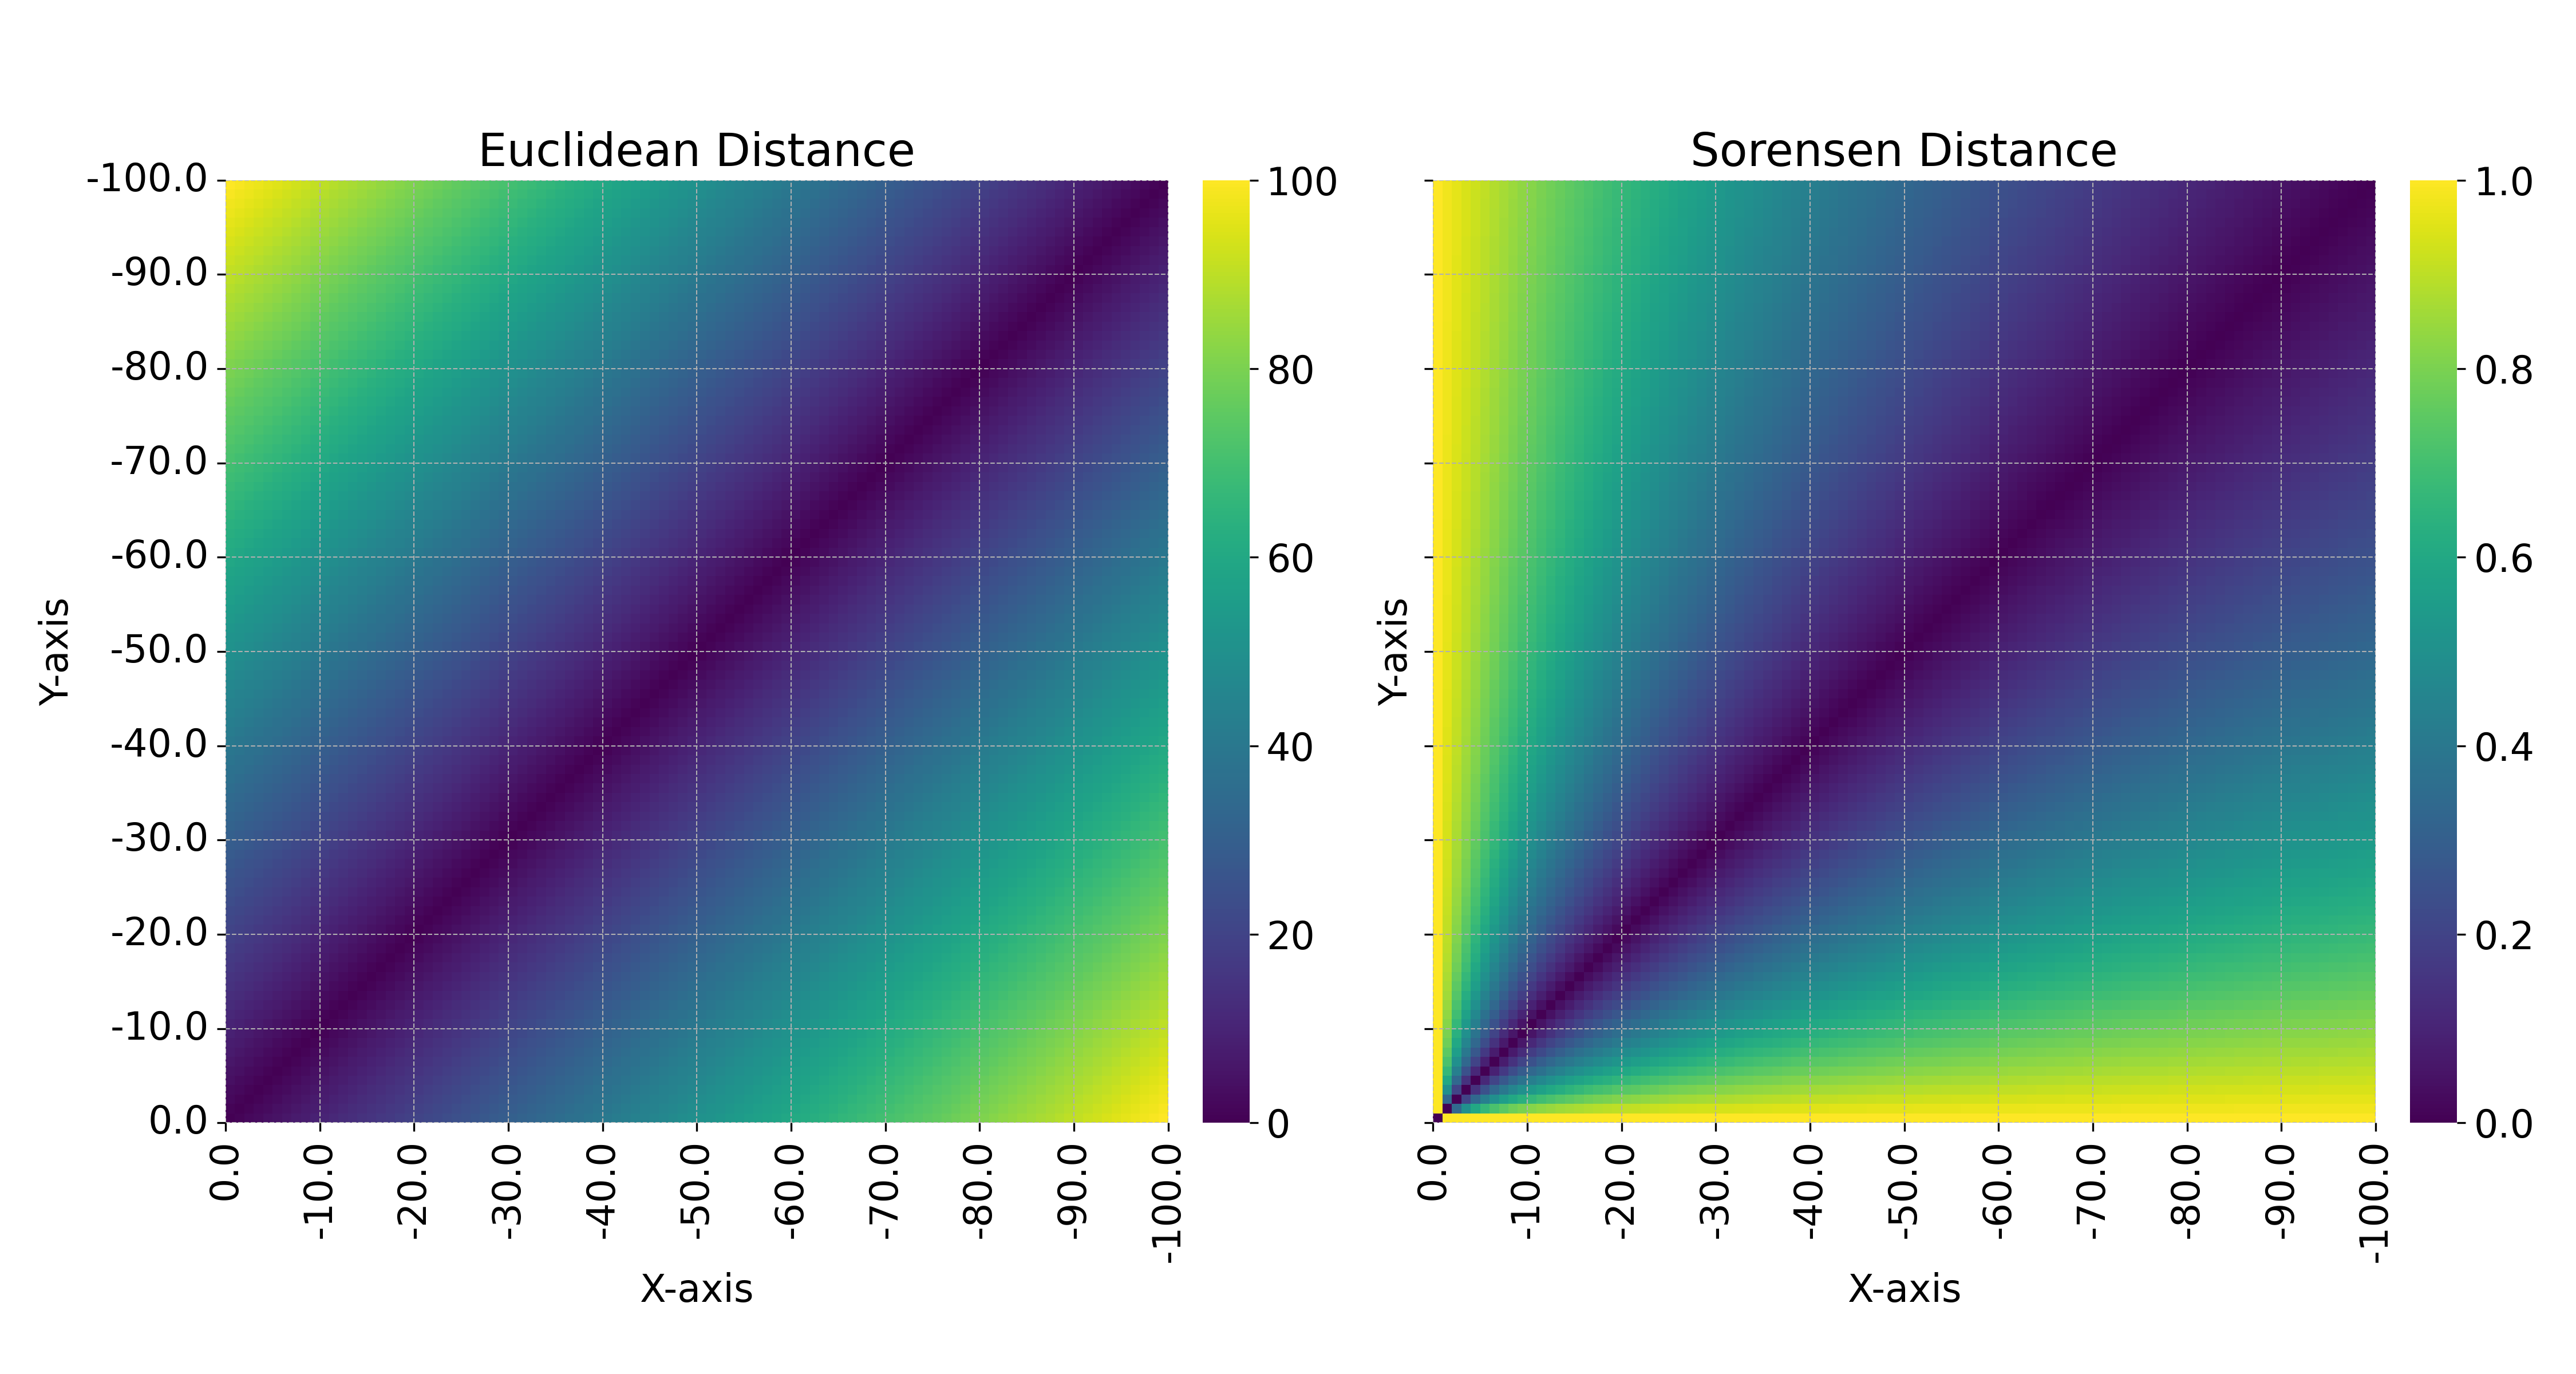
\includegraphics[width=0.8\textwidth]{images/distance_metrics_heatmaps.png}
    \caption{Euclidean vs. Sorensen distance metrics}
    \label{fig:distance_metrics_heatmaps}
\end{figure}



\subsection{Gewichtung (uniform vs. distance)}
\textbf{Quelle 5:}
\begin{itemize}
    \item Die Erweiterung basiert auf der Idee, dass Beobachtungen im Trainingsset, die besonders nahe an der neuen Beobachtung (y, x) liegen, ein höheres Gewicht in der Entscheidungsfindung erhalten sollten als weiter entfernte Nachbarn.
    \item Im klassischen kNN beeinflussen nur die k nächsten Nachbarn die Vorhersage.
    \item Der Einfluss jedes der k nächsten Nachbarn ist gleich, obwohl die individuelle Ähnlichkeit zu (y, x) stark variieren kann.
    \item Um dieses Ziel zu erreichen, müssen die Distanzen, die bei der Suche nach den nächsten Nachbarn im ersten Schritt verwendet werden, in Ähnlichkeitsmaße umgewandelt werden, die als Gewichte verwendet werden können.
\end{itemize}

\subsection{Parameter: Anzahl der Nachbarn}
\textbf{Quelle 1:} Der Parameter k legt fest, wie viele nächste Nachbarn für die Klassifizierung ausgewählt werden. Für k = 1 wird nur der nächste Nachbar ausgewählt, wodurch kein Mehrheitsvotum stattfindet. Bei kleinen Werten für k kann eine hohe Varianz und eine geringe Verzerrung auftreten, während bei größeren Werten die Varianz geringer und die Verzerrung höher ist. Die Auswahl von k hängt stark von den vorhandenen Trainingsdaten ab. Bei Daten mit Ausreißern und Rauschen wird empfohlen, höhere Werte für k zu wählen, da in diesen Fällen bessere Ergebnisse erzielt werden. Zudem wird empfohlen, ungerade Werte für k zu wählen, um Unentschieden beim Mehrheitsvotum zu vermeiden.

\section{Support Vector Machines (SVM)}


In Abbildung \ref{fig:myplot_7_svm} ist ein SVM dargestellt.

\begin{figure}[H]
    \centering
    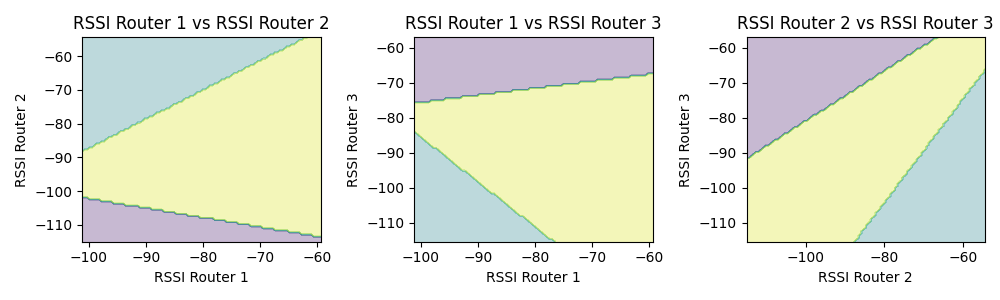
\includegraphics[width=0.8\textwidth]{images/myplot_7_svm.png}
    \caption{SVM}
    \label{fig:myplot_7_svm}
\end{figure}

\textbf{Quellen:} \\
\href{https://www.bigdata-insider.de/was-ist-eine-support-vector-machine-a-880134}{Quelle 6: https://www.bigdata-insider.de/was-ist-eine-support-vector-machine-a-880134} \\
\href{https://www.ibm.com/topics/support-vector-machine}{Quelle 7: https://www.ibm.com/topics/support-vector-machine} \\
\href{https://wires.onlinelibrary.wiley.com/doi/full/10.1002/wics.49}{Quelle 8: https://wires.onlinelibrary.wiley.com/doi/full/10.1002/wics.49}


Quelle warum gerade RBF: An Indoor Localization of WiFi Based on Support Vector Machines

\subsection{Algorithmusbeschreibung}
\textbf{Quelle 7:} Der Support Vector Machine (SVM) Algorithmus ist ein überwachter maschineller Lernalgorithmus, der verwendet wird, um Daten zu klassifizieren. Die Klassifizierung erfolgt, indem die optimale Trennlinie – die sogenannte Hyperebene – zwischen den Datenpunkten gefunden wird. Diese Hyperebene wird so positioniert, dass der maximale Abstand zwischen den Datenpunkten der beiden Klassen erreicht wird. SVM kann sowohl mit linear trennbaren Daten als auch mit nicht linear trennbaren Daten arbeiten. Bei nicht linearen Daten wird der sogenannte Kernel-Trick angewendet, bei dem die Daten mithilfe einer Kernel-Funktion in einen höherdimensionalen Raum transformiert werden.

\subsection{Kernel (linear, RBF)}
\textbf{Quelle 7:} Bei der linearen Klassifizierung werden die Datenpunkte durch eine Linie oder Ebene getrennt und nicht transformiert. Bei nicht linearen SVMs wird zuerst die Kernel-Methode angewendet, und anschließend werden die Daten linear getrennt. In dieser Arbeit wurde entschieden, ein lineares und ein nicht lineares SVM zu vergleichen. Für das nicht lineare SVM wurde der RBF-Kernel gewählt, da in der Arbeit "Device-Free Presence Detection and Localization With SVM and CSI Fingerprinting" mit diesem Kernel die besten Ergebnisse unter den nicht linearen SVMs erzielt wurden.

\subsection{Parameter: Regularisierungsparameter C und Kernel-Parameter gamma}
\textbf{Quelle 7:} Mit dem Parameter C kann der Margin angepasst werden. Ein größerer Wert verengt den Margin für eine minimale Fehlklassifizierung und ein größerer Wert für C erweitert den Margin, sodass mehr Fehlklassifizierungen zugelassen werden. Gamma kontrolliert den Einfluss eines einzelnen Datenpunktes. Ein höherer Wert sorgt für eine kleinere Einflussreichweite, wodurch die Entscheidungsgrenzen enger werden. Der Parameter Gamma kann nur bei nicht linearen SVMs verwendet werden. \\
Quelle für die Auswahl der Parameter Werte: Semi-Supervised Classification by Low Density Separation

\section{Random Forest}

Gute quelle: WiFi Indoor Localization with CSI Fingerprinting-Based Random Forest -> Wie wichtig ist welcher Hyperparameter?

In Abbildung \ref{fig:myplot_7_rf} ist ein Entscheidungsbaum dargestellt.

\begin{figure}[H]
    \centering
    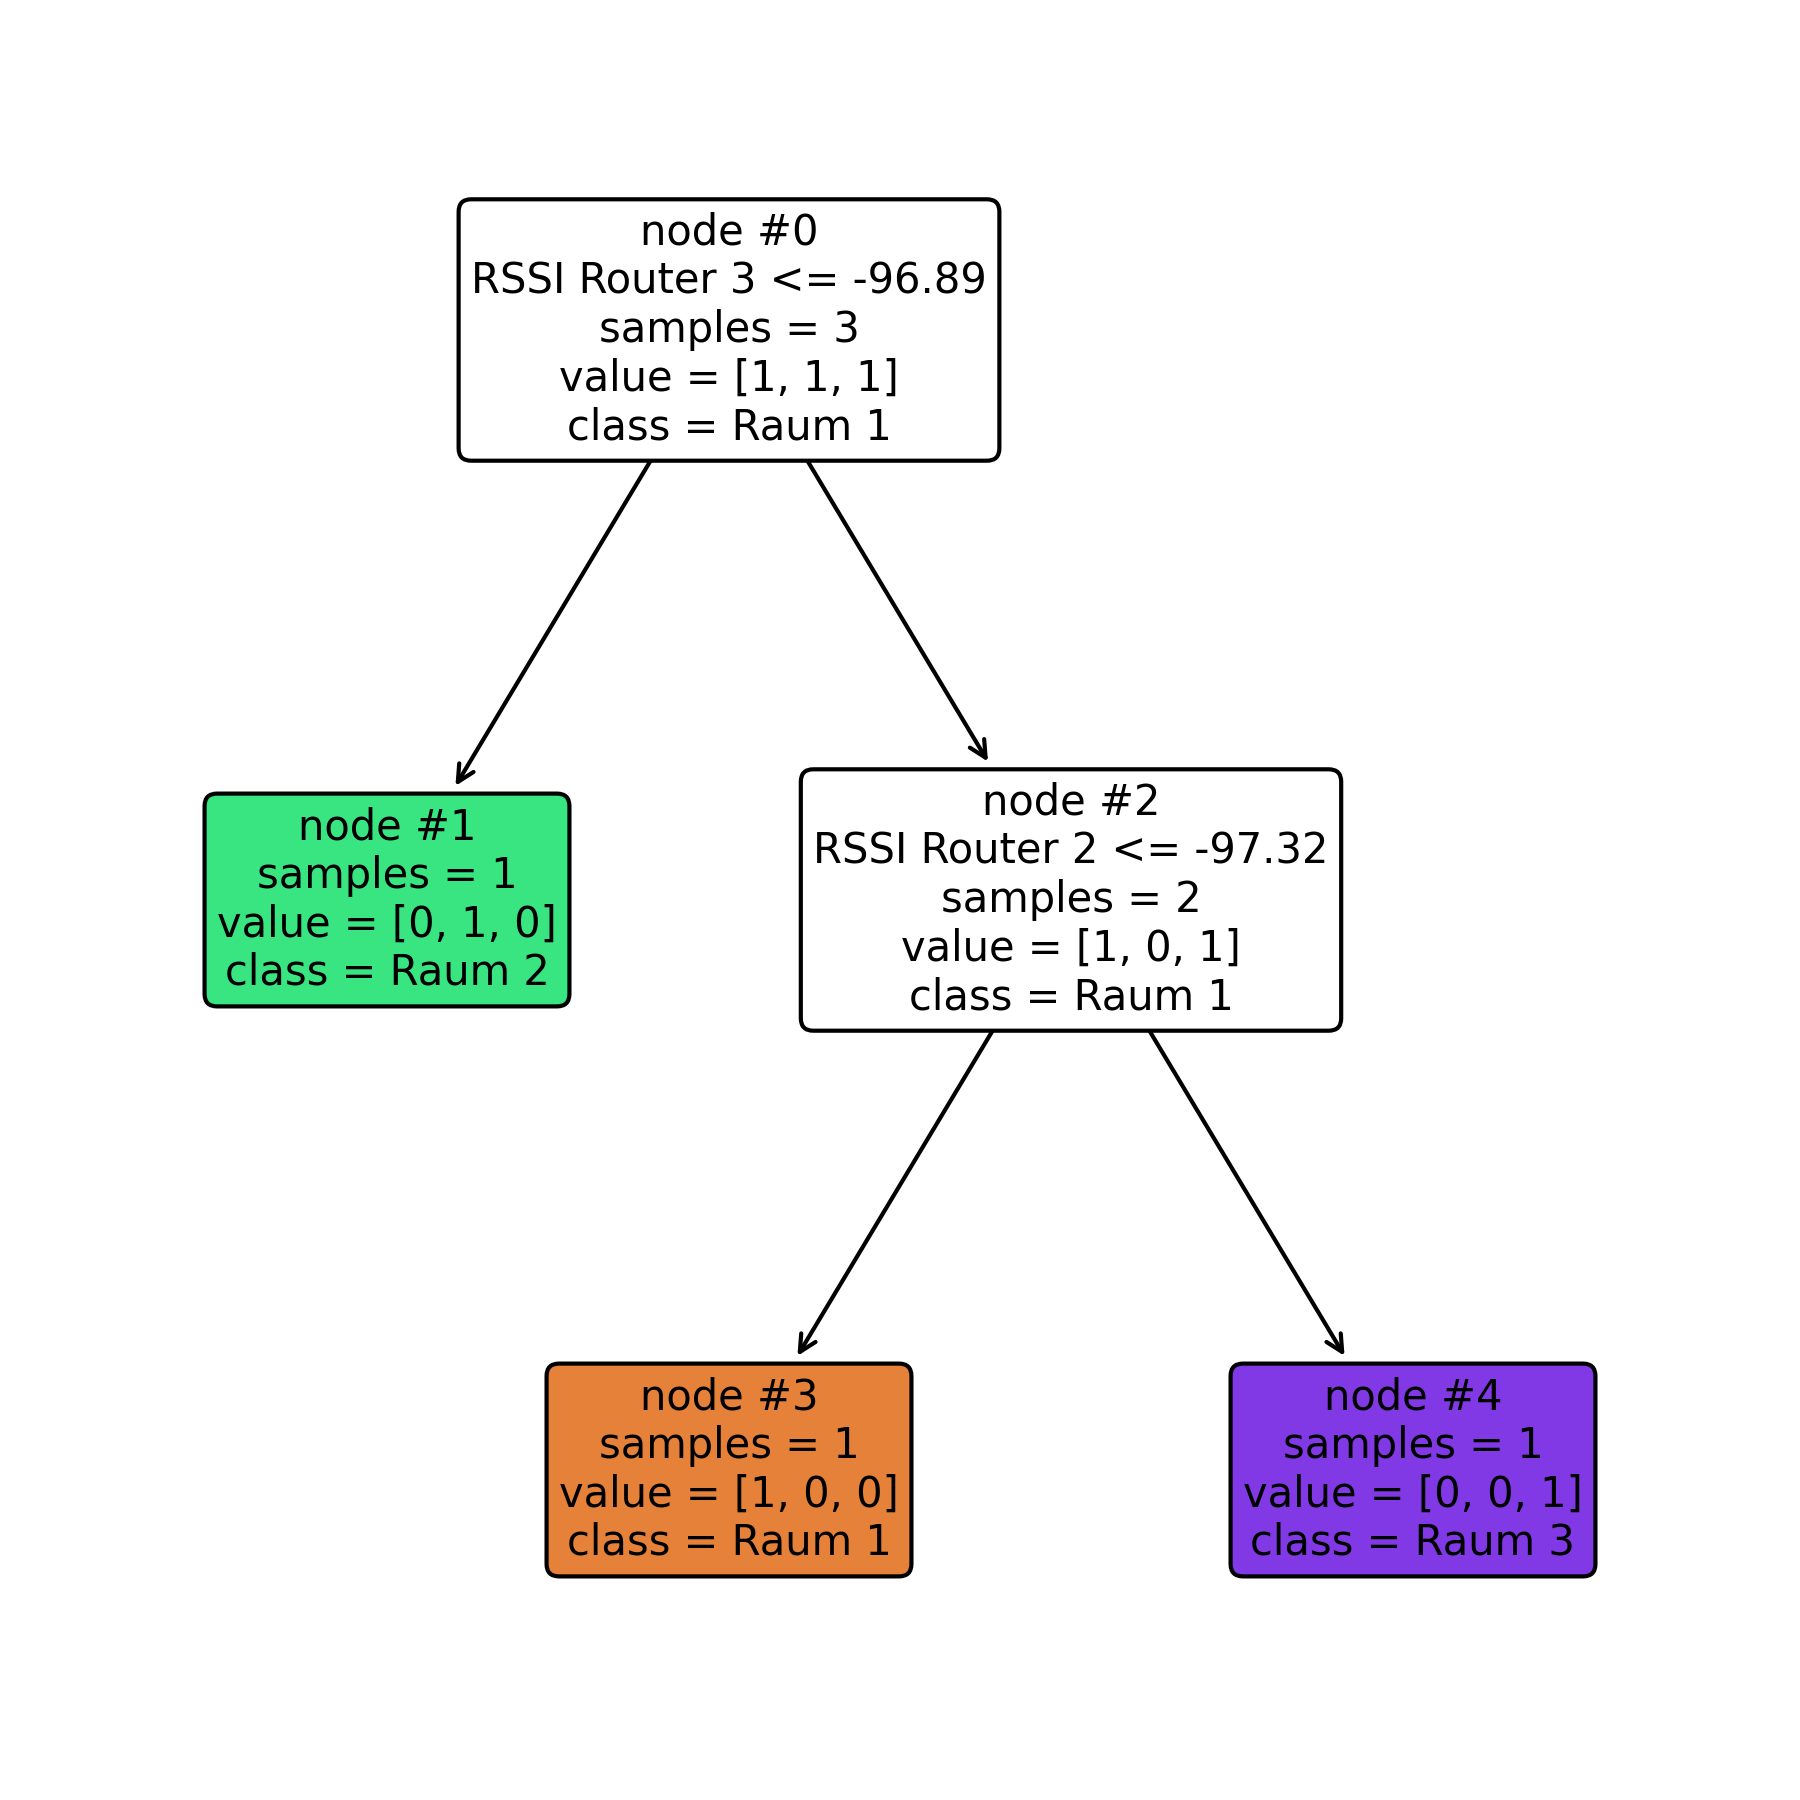
\includegraphics[width=0.8\textwidth]{images/myplot_7_rf.png}
    \caption{Distance vs. Uniform weights}
    \label{fig:myplot_7_rf}
\end{figure}

\textbf{Quelle:} \\
\href{https://builtin.com/data-science/random-forest-algorithm}{Quelle 9: https://builtin.com/data-science/random-forest-algorithm}

\subsection{Algorithmusbeschreibung}
\textbf{Quelle 9:} Der Random Forest Algorithmus ist ein überwachter Lernalgorithmus, der eine Menge an Entscheidungsbäumen erstellt. Ein Entscheidungsbaum besteht aus Knoten, welche eine Bedingung zu einem der Merkmale aus dem Datenset abfragen. Zum Beispiel sowas wie: Ist der RSSI-Wert von Access Point 1 größer gleich -80 dBm? Je nachdem wie diese Frage beantwortet wird, geht es dann zum nächsten Knoten usw. Am Ende jedes Strangs

\subsection{Parameter: Anzahl der Bäume (n\_estimators)}

\chapter{Systemarchitektur und Implementierung}
\section{Architekturübersicht (App, API, Datenbank)}

\subsection{Implementierung der Android App (BVG Detection)}
\begin{itemize}
    \item \textbf{App-Architektur:} Geben Sie eine Übersicht über die Architektur der Android-App und deren Hauptkomponenten.
    \item \textbf{Funktionalitäten:} Beschreiben Sie die Hauptfunktionen der App, einschließlich Fingerprint-Aufnahme und Raumvorhersage.
    \item \textbf{Technologien und Bibliotheken:} Erklären Sie die verwendeten Technologien und Bibliotheken zur Implementierung der App.
\end{itemize}

\subsection{Implementierung der API}

Die API wurde mithilfe des Frameworks Flask entwickelt und läuft auf der virtuellen Maschine

\begin{itemize}
    \item \textbf{API-Design:} Die API wurde mit Flask entwickelt und dient der Verwaltung und Abfrage von WiFi-Fingerprints zur Indoor-Ortung. Die Hauptendpunkte sind:
          \begin{itemize}
              \item \texttt{/measurements} (POST): Hinzufügen eines neuen Fingerprints.
              \item \texttt{/measurements/batch} (POST): Hinzufügen mehrerer Fingerprints im Batch.
              \item \texttt{/measurements/all} (GET): Abrufen aller gespeicherten Fingerprints.
              \item \texttt{/measurements/reset} (POST): Zurücksetzen aller gespeicherten Fingerprints und zugehöriger Daten.
              \item \texttt{/measurements/predict} (POST): Vorhersage des Raumes basierend auf empfangenen WiFi-Daten.
              \item \texttt{/ping} (GET): Überprüfen, ob der Server läuft.
              \item \texttt{/measurements/room\_names} (GET): Abrufen aller Messungs-IDs mit ihren zugehörigen Raumnamen.
          \end{itemize}
          Jeder Endpunkt hat eine spezifische Funktion und dient entweder der Datenspeicherung, -abfrage oder -vorhersage.

    \item \textbf{Funktionalitäten:} Die API bietet folgende Hauptfunktionen:
          \begin{itemize}
              \item \textbf{Fingerprint-Speicherung:} Die Funktion \texttt{handle\_add\_measurement} ermöglicht das Hinzufügen eines neuen Fingerprints zur Datenbank. Hierbei werden Informationen wie Raumname, Geräte-ID, Zeitstempel und Routerdaten gespeichert.
              \item \textbf{Batch-Speicherung:} Mit der Funktion \texttt{handle\_add\_measurements\_batch} können mehrere Fingerprints in einem Schritt hinzugefügt werden, was die Effizienz bei der Datenerfassung erhöht.
              \item \textbf{Raumvorhersage:} Die Funktion \texttt{handle\_predict\_room} verwendet verschiedene Machine Learning Algorithmen (KNN, Random Forest, SVM), um basierend auf empfangenen WiFi-Daten den wahrscheinlichsten Raum vorherzusagen. Hierbei werden verschiedene Parameter wie der Algorithmus, die Anzahl der Nachbarn (k-Wert) und Gewichtungsstrategien berücksichtigt.
              \item \textbf{Datenabfrage:} Über die Endpunkte \texttt{/measurements/all} und \texttt{/measurements/room\_names} können alle gespeicherten Fingerprints sowie die zugehörigen Raumnamen abgerufen werden.
              \item \textbf{Daten-Reset:} Mit \texttt{handle\_reset\_measurements} können alle gespeicherten Fingerprints und zugehörige Daten zurückgesetzt werden, was besonders bei Testläufen nützlich ist.
          \end{itemize}

    \item \textbf{Sicherheitsaspekte:} Die API berücksichtigt verschiedene Sicherheitsaspekte, um den Schutz der Daten zu gewährleisten:
          \begin{itemize}
              \item \textbf{Authentifizierung und Autorisierung:} Um sicherzustellen, dass nur autorisierte Benutzer auf die API zugreifen und Änderungen vornehmen können, sollten Authentifizierungs- und Autorisierungsmechanismen wie API-Schlüssel oder OAuth implementiert werden. In der aktuellen Implementierung fehlt diese Funktionalität und sollte daher als zukünftige Verbesserung berücksichtigt werden.
              \item \textbf{Datenvalidierung:} Bei der Verarbeitung eingehender Anfragen wird die Integrität der Daten überprüft. Fehlende oder fehlerhafte Daten führen zu Fehlermeldungen und die Anfragen werden abgelehnt (z.B. \texttt{handle\_add\_measurement} überprüft, ob alle erforderlichen Felder vorhanden sind).
              \item \textbf{Logging und Monitoring:} Die API enthält Logging-Funktionalitäten, die Informationen über eingehende Anfragen und ausgehende Antworten protokollieren. Dies hilft bei der Überwachung der API-Nutzung und beim Debugging.
              \item \textbf{Fehlerbehandlung:} Die API behandelt verschiedene Fehlerzustände, wie z.B. das Überschreiten der Zeitlimits für Anfragen oder Netzwerkprobleme, und liefert entsprechende Fehlermeldungen an den Client.
          \end{itemize}
\end{itemize}


\section{Datenbankstruktur (MariaDB, SQLite)}

Es wurde eine relationale Datenbank gewählt, da viele Einträge wie Räume und Router mehrfach vorkommen und so die größe der Datenbank nicht linear wächst mit jeder neuen Messung.

Die entwickelte Datenbankstruktur besteht aus vier zentralen Tabellen: \textit{rooms}, \textit{measurements}, \textit{routers} und \textit{measurement\_router}. Diese Struktur wurde gewählt, um eine effiziente und flexible Speicherung sowie Verwaltung der für die Raumbestimmung erforderlichen Daten zu gewährleisten. Die einzelnen Tabellen und deren Beziehungen sind in Abbildung \ref{fig:database-structure} dargestellt.

\begin{figure}[h]
    \centering
    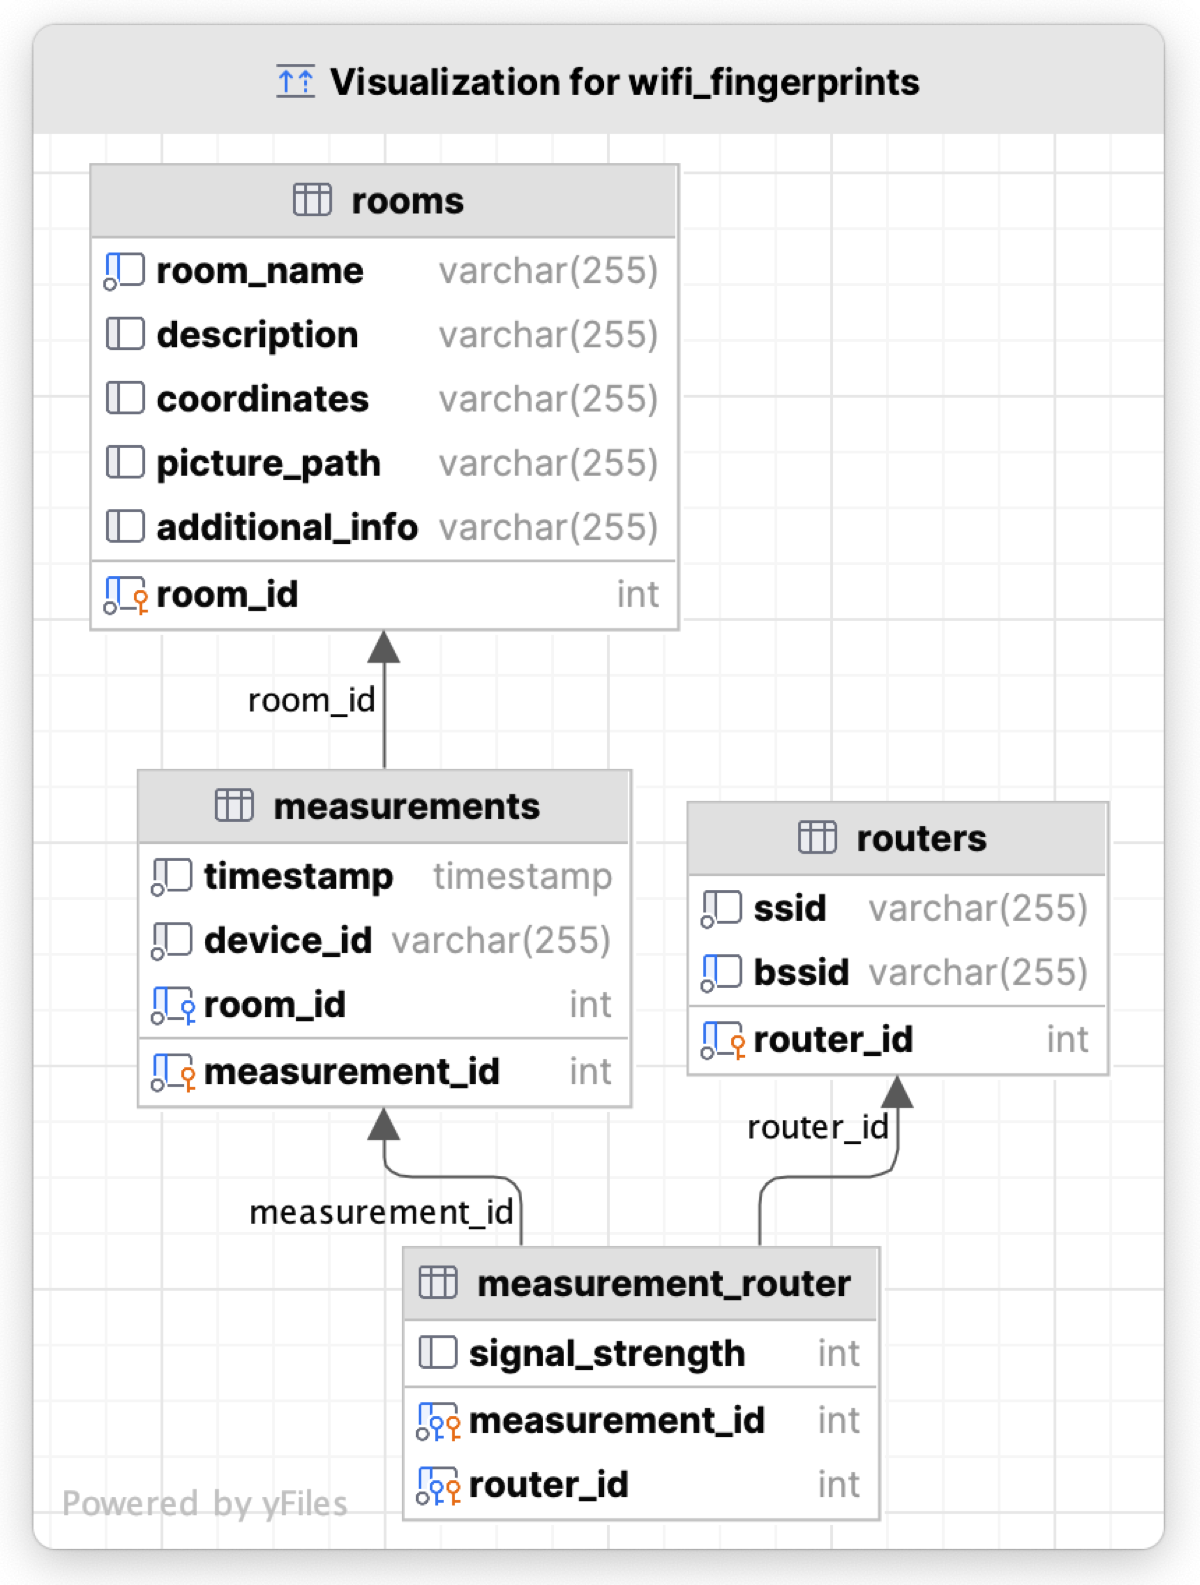
\includegraphics[width=0.3\textwidth]{images/database_strucure.png}
    \caption{Datenbankstruktur}
    \label{fig:database-structure}
\end{figure}

\begin{figure}
    \centering
    \begin{tikzpicture}[
        table/.style={rectangle split, rectangle split parts=6, draw, rounded corners, text centered, minimum height=4em, minimum width=12em, inner sep=2pt},
        link/.style={draw, -{Latex[length=3mm]}, thick},
        reversedlink/.style={draw, {Latex[length=3mm]}-, thick},
        every node/.style={font=\small},
        nodes in empty cells
        ]

        % Matrix
        \matrix (m) [matrix of nodes, row sep=2cm, column sep=2cm, nodes={table},
            column 1/.style={anchor=center},
            column 2/.style={anchor=center}] {
            \node[table, rectangle split parts=7] (rooms) {
                \textbf{rooms}
                \nodepart{two} room\_id : int
                \nodepart{three} room\_name : varchar(255)
                \nodepart{four} description : varchar(255)
                \nodepart{five} coordinates : varchar(255)
                \nodepart{six} picture\_path : varchar(255)
                \nodepart{seven} additional\_info : varchar(255)
            }; &
            \node[table, rectangle split parts=4] (routers) {
                \textbf{routers}
                \nodepart{two} router\_id : int
                \nodepart{three} ssid : varchar(255)
                \nodepart{four} bssid : varchar(255)
            };            \\
            \node[table, rectangle split parts=5] (measurements) {
                \textbf{measurements}
                \nodepart{two} measurement\_id : int
                \nodepart{three} timestamp : timestamp
                \nodepart{four} device\_id : varchar(255)
                \nodepart{five} room\_id : int
            };     &
            \node[table, rectangle split parts=4] (measurement_router) {
                \textbf{measurement\_router}
                \nodepart{two} signal\_strength : int
                \nodepart{three} measurement\_id : int
                \nodepart{four} router\_id : int
            }; \\
        };

        % Links
        \draw[link] (measurement_router.north) -- (routers.south);
        \draw[link] (measurement_router.west) -| ([xshift=-1.5cm]measurement_router.west) |- (measurements.east);
        \draw[link] (measurements.north) -- (rooms.south);

    \end{tikzpicture}
    \caption{Diagramm der Datenbanktabellen und ihrer Beziehungen}
    \label{fig:database-diagram}
\end{figure}


\subsection{Tabelle \textit{rooms}}

Die Tabelle \textit{rooms} speichert Informationen über alle aufgenommenen Räume. Sie enthält die folgenden Felder:
\begin{itemize}
    \item \textit{room\_id}: Primärschlüssel, der automatisch inkrementiert wird.
    \item \textit{room\_name}: Name des Raumes, der eindeutig sein muss.
    \item \textit{description}: Beschreibung des Raumes.
    \item \textit{coordinates}: Koordinaten des Raumes.
    \item \textit{picture\_path}: Pfad zu einem Bild des Raumes.
    \item \textit{additional\_info}: Weitere Informationen zum Raum.
\end{itemize}

Die Felder \textit{description}, \textit{coordinates}, \textit{picture\_path} und \textit{additional\_info} sind vorhanden, da die Datenbank auch auf mobilen Geräten läuft und die App diese Daten speichert. Dies ermöglicht eine umfassende Dokumentation und einfache Identifikation der Räume.

\subsection{Tabelle \textit{measurements}}

In der Tabelle \textit{measurements} werden alle Messungen gespeichert. Die Felder umfassen:
\begin{itemize}
    \item \textit{measurement\_id}: Primärschlüssel, der automatisch inkrementiert wird.
    \item \textit{timestamp}: Zeitstempel der Messung.
    \item \textit{device\_id}: Kennung des Geräts, das die Messung durchgeführt hat.
    \item \textit{room\_id}: Fremdschlüssel, der auf die \textit{room\_id} in der Tabelle \textit{rooms} verweist.
\end{itemize}

Bei der Hinzufügung einer neuen Messung wird überprüft, ob der Raum bereits existiert und gegebenenfalls hinzugefügt. Ebenso wird überprüft, ob der Router bereits in der Tabelle \textit{routers} vorhanden ist.

\subsection{Tabelle \textit{routers}}

Die Tabelle \textit{routers} enthält Informationen zu allen Routern, die bei den Messungen erfasst wurden:
\begin{itemize}
    \item \textit{router\_id}: Primärschlüssel, der automatisch inkrementiert wird.
    \item \textit{ssid}: SSID des Routers.
    \item \textit{bssid}: BSSID des Routers, die eindeutig sein muss.
\end{itemize}

Die Eindeutigkeit der BSSID wird durch einen einzigartigen Schlüssel sichergestellt. Dies ist notwendig, um sicherzustellen, dass jeder Router nur einmal in der Datenbank gespeichert wird.

\subsection{Tabelle \textit{measurement\_router}}

Die Tabelle \textit{measurement\_router} stellt die Beziehung zwischen den Messungen und den Routern dar und speichert die Signalstärke:
\begin{itemize}
    \item \textit{measurement\_id}: Fremdschlüssel, der auf die \textit{measurement\_id} in der Tabelle \textit{measurements} verweist.
    \item \textit{router\_id}: Fremdschlüssel, der auf die \textit{router\_id} in der Tabelle \textit{routers} verweist.
    \item \textit{signal\_strength}: Signalstärke, die bei der Messung erfasst wurde.
\end{itemize}

Die Primärschlüssel der Tabelle \textit{measurement\_router} bestehen aus der Kombination von \textit{measurement\_id} und \textit{router\_id}, um sicherzustellen, dass jede Kombination aus Messung und Router nur einmal gespeichert wird.

\subsection{Validierung und Vermeidung von Duplikaten}

Um zu verhindern, dass Messungen doppelt hinzugefügt werden, wird überprüft, ob bereits eine Messung mit derselben \textit{device\_id} und demselben \textit{timestamp} existiert. Dies stellt sicher, dass jede Messung einzigartig ist und keine redundanten Daten in der Datenbank gespeichert werden.

Zusammenfassend bietet die gewählte Datenbankstruktur eine robuste Grundlage für die Speicherung und Verwaltung der Daten, die für die Raumbestimmung mittels WiFi Fingerprints erforderlich sind. Die Struktur ermöglicht eine effiziente Verarbeitung und Abfrage der Daten, was für die Echtzeitanwendung in mobilen Geräten essenziell ist.

\subsection{MariaDB auf der VM}
\begin{itemize}
    \item \textbf{Datenbankdesign:} Beschreiben Sie das Design der MariaDB-Datenbank und die wichtigsten Tabellen.
    \item \textbf{Speicherung von Fingerprints:} Erklären Sie, wie Fingerprint-Daten in der MariaDB gespeichert und verwaltet werden.
    \item \textbf{Abfragen und API-Interaktion:} Diskutieren Sie die wichtigsten Abfragen und die Interaktion mit der API.
\end{itemize}

\subsection{SQLite auf den mobilen Geräten}
\begin{itemize}
    \item \textbf{Datenbankdesign:} Beschreiben Sie das Design der SQLite-Datenbank und die wichtigsten Tabellen.
    \item \textbf{Lokal gespeicherte Daten:} Erklären Sie, welche Daten lokal auf den mobilen Geräten gespeichert werden und warum.
    \item \textbf{Synchronisation mit MariaDB:} Diskutieren Sie die Mechanismen zur Synchronisation der SQLite-Daten mit der MariaDB.
\end{itemize}

\section{Implementierung der Android App (BVG Detection)}
\subsection{Wiederinbetriebnahme der App}

TODO: Aus der ersten Version holen...

\subsection{Gerätekompatibilität und allgemeine Informationen}

TODO: Welche Versionen werden unterstützt (Android/SDK...)

\subsection{Aufnahme von WiFi-Fingerprints}

TODO: Screenshots bei der Aufnahme von Fingerprints und mit der Liste der Fingerprints

\subsection{Datenaustausch}

\section{Bluetooth-Datenaustausch zwischen Geräten}
\begin{itemize}
    \item \textbf{Funktionalität:} Der Bluetooth-Datenaustausch zwischen Geräten ermöglicht es, WiFi-Fingerprints direkt zwischen zwei Geräten auszutauschen, ohne eine zentrale Datenbank oder API verwenden zu müssen. Dies ist besonders nützlich, wenn eine schnelle und lokale Synchronisation der Daten erforderlich ist, beispielsweise in Umgebungen ohne Internetzugang. Die Bluetooth-Kommunikation ermöglicht es, dass Gerät A Fingerprints an Gerät B senden kann und umgekehrt. Dies erweitert die Flexibilität und Anwendungsmöglichkeiten der App erheblich.

    \item \textbf{Technische Umsetzung:} Die technische Umsetzung des Bluetooth-Datenaustauschs in der Android-App erfolgt durch die Verwendung der BluetoothAdapter- und BluetoothSocket-Klassen von Android. Der Prozess beinhaltet die folgenden Schritte:
          \begin{itemize}
              \item \textbf{Initialisierung:} Der BluetoothAdapter wird initialisiert, um das Bluetooth-Modul des Geräts zu steuern. Falls Bluetooth nicht aktiviert ist, wird der Benutzer aufgefordert, es zu aktivieren.
              \item \textbf{Paaren von Geräten:} Eine Liste der gekoppelten Bluetooth-Geräte wird angezeigt, und der Benutzer kann ein Gerät auswählen, mit dem eine Verbindung hergestellt werden soll.
              \item \textbf{Verbindung herstellen:} Die App startet einen Server-Socket (AcceptThread) auf einem Gerät, der auf eingehende Verbindungen wartet. Ein anderes Gerät kann sich mit diesem Server-Socket verbinden (ConnectThread).
              \item \textbf{Datenübertragung:} Nachdem die Verbindung hergestellt ist, wird ein ConnectedThread gestartet, der die Datenübertragung verwaltet. Die Fingerprint-Daten werden in JSON-Format konvertiert und in Blöcken über die Bluetooth-Verbindung gesendet. Der Empfang und das Zusammenfügen der Daten erfolgt ebenfalls in diesem Thread.
              \item \textbf{Verarbeitung empfangener Daten:} Die empfangenen Daten werden geparst und in die lokale SQLite-Datenbank eingefügt oder aktualisiert. Der BluetoothHelper kümmert sich um die Verarbeitung der empfangenen JSON-Daten und deren Integration in die bestehende Datenbankstruktur.
          \end{itemize}

    \item \textbf{Anwendungsfälle:} Der Bluetooth-Datenaustausch bietet mehrere Vorteile und Anwendungsfälle:
          \begin{itemize}
              \item \textbf{Schnelle lokale Synchronisation:} Ideal für Umgebungen ohne Internetzugang, da die Daten direkt zwischen den Geräten ausgetauscht werden können.
              \item \textbf{Datensicherung und -wiederherstellung:} Ein Benutzer kann seine Fingerprint-Daten auf ein anderes Gerät übertragen, um eine Datensicherung zu erstellen oder Daten wiederherzustellen.
              \item \textbf{Kollaborative Datensammlung:} Mehrere Benutzer können parallel Fingerprint-Daten sammeln und diese anschließend miteinander teilen, um eine umfassendere Datenbasis zu schaffen.
              \item \textbf{Redundanz und Ausfallsicherheit:} Durch den Austausch der Daten zwischen Geräten wird sichergestellt, dass die Daten auch bei einem Geräteausfall nicht verloren gehen.
          \end{itemize}
\end{itemize}

\subsection{Standortbestimmung}

TODO: Screenshots mit den Einstellungen, dem erfolgreichen Ergenis


\section{Implementierung der API und Datenbank}

Hier kommt eig. der Teil hin der aktuell in Implementierung der API steht.

\subsection{API-Endpunkte und Kommunikation}

TODO: Liste aller Endpunkte..

\subsection{Code-Integration des ESP32 für die Standortbestimmung}

TODO: Code des ESP32, MicroPythin ist toll

\chapter{Datenerhebung und -analyse}
\section{Datensammlung und -aufbereitung}
\subsection{Beschreibung der gesammelten Daten}

\begin{itemize}
    \item \textbf{Datenerhebungsmethoden:} Erklären Sie, wie die Daten gesammelt wurden (z.B. welche Geräte, Orte und Zeitpunkte).
    \item \textbf{Datensätze und Umfang:} Beschreiben Sie den Umfang und die Struktur der gesammelten Datensätze.
    \item \textbf{Datenqualität und -validität:} Diskutieren Sie die Qualität und Validität der Daten.
\end{itemize}

Es wurden insgesamt 407 Messungen in 35 Räumen durchgeführt. Die Messungen wurden zwischen dem 8. Mai 2024 und dem 31. Mai 2024 durchgeführt. Im Schnitt wurden bei jeder Messung 12,8 Router erfasst. Im Schnitt wurden 11,6 Messungen pro Raum durchgeführt. Die Anzahl der Messungen pro Raum variiert zwischen 2 und 19. Es wurden insgesamt 318 Router erfasst.

Die Anzahl der Messungen pro Raum sind in Abbildung \ref{fig:0_general_01} dargestellt.

\begin{figure}[H]
    \centering
    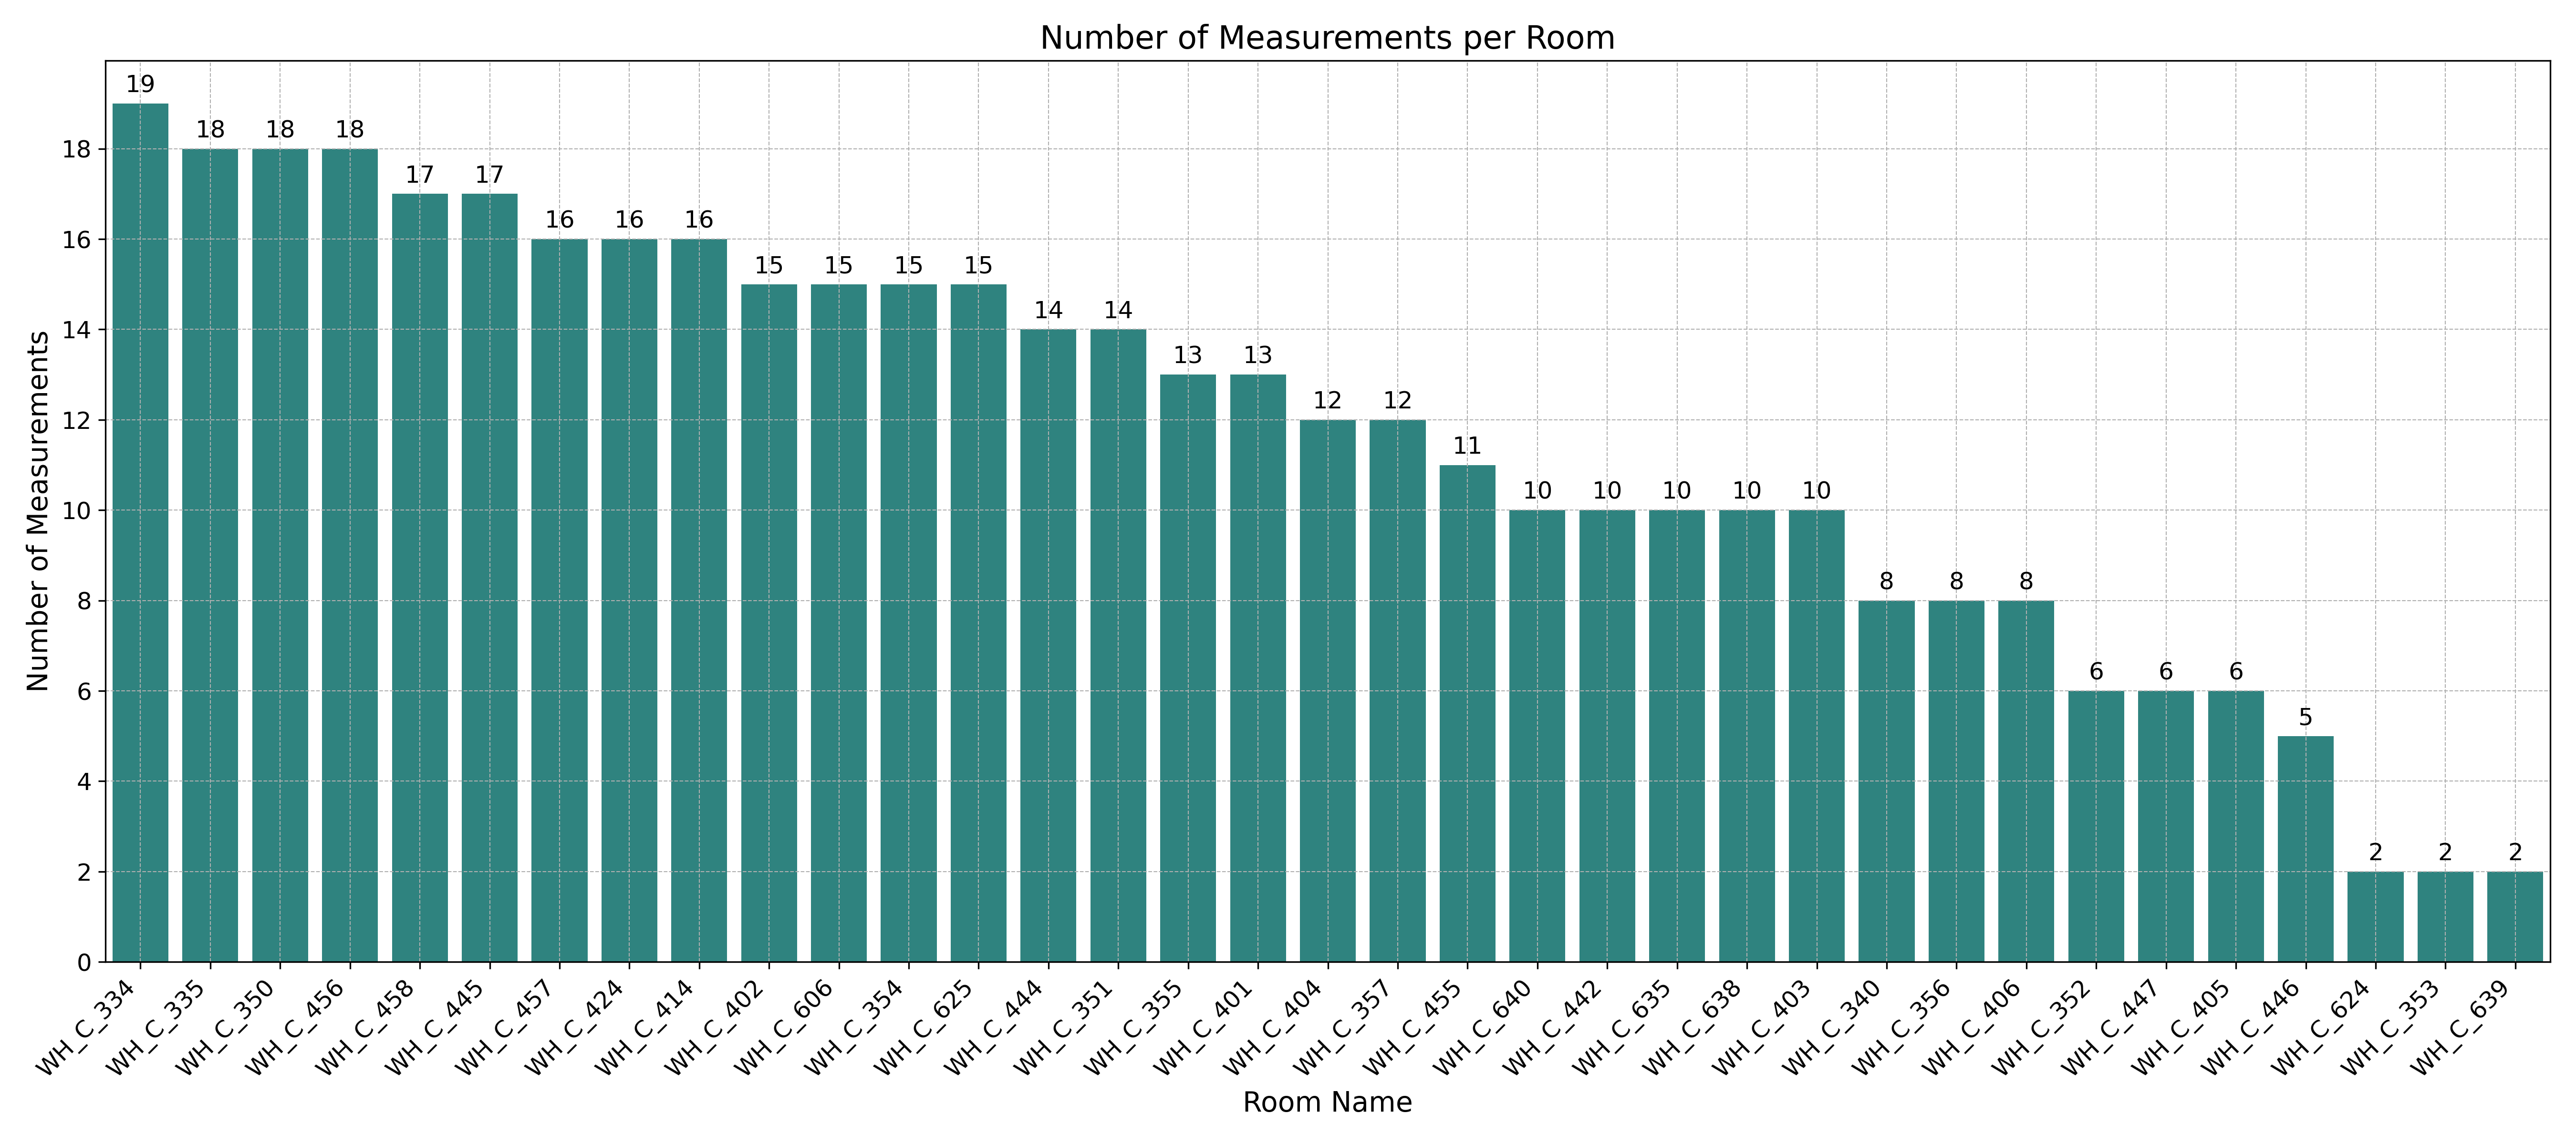
\includegraphics[width=0.8\textwidth]{images/0_general_01.png}
    \caption{Beispielabbildung 1}
    \label{fig:0_general_01}
\end{figure}

\begin{itemize}
    \item Verwendete Geräte (Doogee Y8, Google Pixel 8, Samsung Galaxy A?!)
\end{itemize}

\subsection{Methodik zur Untersuchung der Algorithmen}
\subsection{Detaillierte Beschreibung des Testprogramms}

\begin{itemize}
    \item \textbf{Programmübersicht:} Das Testprogramm dient dazu, die Leistungsfähigkeit verschiedener Machine Learning Algorithmen zur Indoor-Ortung basierend auf WiFi-Fingerprints zu evaluieren. Es lädt Konfigurationsparameter aus einer YAML-Datei, ruft Daten von einer API ab, filtert diese nach bestimmten Kriterien und vergleicht die Vorhersagen der Algorithmen unter verschiedenen Parametereinstellungen. Die Ergebnisse werden anschließend in CSV-Dateien gespeichert.

    \item \textbf{Ablauf und Logik:} Der Ablauf des Programms lässt sich wie folgt zusammenfassen:
          \begin{itemize}
              \item \textbf{Konfiguration laden:} Mit der Funktion \texttt{load\_config} wird die Konfigurationsdatei \texttt{config.yaml} geladen, die alle notwendigen Einstellungen und Parameter für die Tests enthält.
              \item \textbf{Erstellen des Ausgabeordners:} Die Funktion \texttt{create\_output\_directory} erstellt einen neuen Ordner, in dem die Ergebnisse gespeichert werden. Der Ordnername enthält einen Zeitstempel, um die Ergebnisse eindeutig zu identifizieren.
              \item \textbf{Daten abrufen:} Die Funktion \texttt{fetch\_data} ruft die WiFi-Fingerprint-Daten von einer angegebenen URL ab.
              \item \textbf{Daten filtern:} Falls in der Konfiguration Räume oder Korridore angegeben sind, werden die Daten mit der Funktion \texttt{filter\_data} entsprechend gefiltert.
              \item \textbf{Parameterkombinationen generieren:} Mit der Funktion \texttt{gene\allowbreak rate\_para\allowbreak meter\_\allowbreak com\allowbreak bi\allowbreak nations} werden alle möglichen Kombinationen der angegebenen Parameterwerte erstellt.
              \item \textbf{Vorhersagen und Vergleiche:} Die Funktion \texttt{compare\_predictions} vergleicht die Vorhersagen der Algorithmen mit den tatsächlichen Raumdaten. Die Ergebnisse werden in CSV-Dateien gespeichert, wobei jede Datei eine spezifische Parametereinstellung repräsentiert.
          \end{itemize}

    \item \textbf{Erweiterbarkeit und Anpassung:} Das Programm ist so aufgebaut, dass es leicht erweitert und angepasst werden kann. Neue Parameter oder Algorithmen können einfach in die YAML-Konfigurationsdatei hinzugefügt werden. Die modularen Funktionen ermöglichen es, einzelne Teile des Programms bei Bedarf zu modifizieren oder zu ersetzen, ohne die gesamte Codebasis ändern zu müssen.
\end{itemize}

\subsubsection{Konfiguration über YAML-Dateien}
\begin{itemize}
    \item \textbf{Konfigurationsdateien:} Die Konfiguration des Programms erfolgt über eine YAML-Datei (\texttt{config.yaml}), die alle notwendigen Parameter und Einstellungen enthält. Diese Datei ermöglicht eine flexible Anpassung des Testprozesses, ohne dass der Quellcode selbst verändert werden muss.

    \item \textbf{Parameter und Einstellungen:} Die YAML-Datei enthält folgende Hauptparameter:
          \begin{itemize}
              \item \textbf{url\_fetch:} Die URL, von der die WiFi-Fingerprint-Daten abgerufen werden.
              \item \textbf{url\_predict:} Die URL der API, die für die Vorhersagen verwendet wird.
              \item \textbf{num\_measurements:} Die Anzahl der Messungen, die verarbeitet werden sollen.
              \item \textbf{rooms und corridors:} Listen von Raum- und Korridornamen, die in die Analyse einbezogen werden sollen.
              \item \textbf{parameter\_sets:} Verschiedene Sätze von Parametern, die für die Vorhersagen verwendet werden. Jeder Satz enthält spezifische Werte für Algorithmen und deren Einstellungen.
          \end{itemize}

    \item \textbf{Anwendungsbeispiele:} Ein typisches Beispiel für die YAML-Konfigurationsdatei sieht wie folgt aus:
          \begin{lstlisting}[caption=.yaml Konfigurationsdatei, label={lst:code_yaml}]
url_fetch: "http://127.0.0.1:5000/measurements/all"
url_predict: "http://127.0.0.1:5000/measurements/predict"
num_measurements: 10
rooms: ["WH_C_334", "WH_C_335"]
corridors: ["WH_C_352"]
parameter_sets:
    - name: "test"
    parameters:
        router_selection: ['all']
        handle_missing_values_strategy: ['-100']
        router_presence_threshold: [0]
        router_rssi_threshold: [-100]
        value_scaling_strategy: ['none']
        weights: ["distance"]
        algorithm:
            knn_euclidean:
                k_value: [7]
        \end{lstlisting}
          Diese Konfiguration spezifiziert, dass die Daten von \texttt{http://127.0.0.1:5000/\discretionary{}{}{}measure\discretionary{}{}{}ments/\discretionary{}{}{}all} abgerufen und die Vorhersagen bei \texttt{http://127.0.0.1:5000/\discretionary{}{}{}measure\discretionary{}{}{}ments/\discretionary{}{}{}predict} gemacht werden sollen. Es sollen 10 Messungen verarbeitet werden, die entweder in den angegebenen Räumen oder Korridoren aufgenommen wurden. Der Parameter \texttt{parameter\_sets} definiert verschiedene Sätze von Parametern, die für die Vorhersagen verwendet werden.
\end{itemize}



\section{Vergleich der Algorithmen und Parameter}
\subsection{Untersuchung der Genauigkeit in Abhängigkeit von Parametern}

1. Auswahl der nicht konkret betrachteten Parameter bei KNN und SVM

KNN (weights: distance vs. uniform):

\begin{figure}[H]
    \centering
    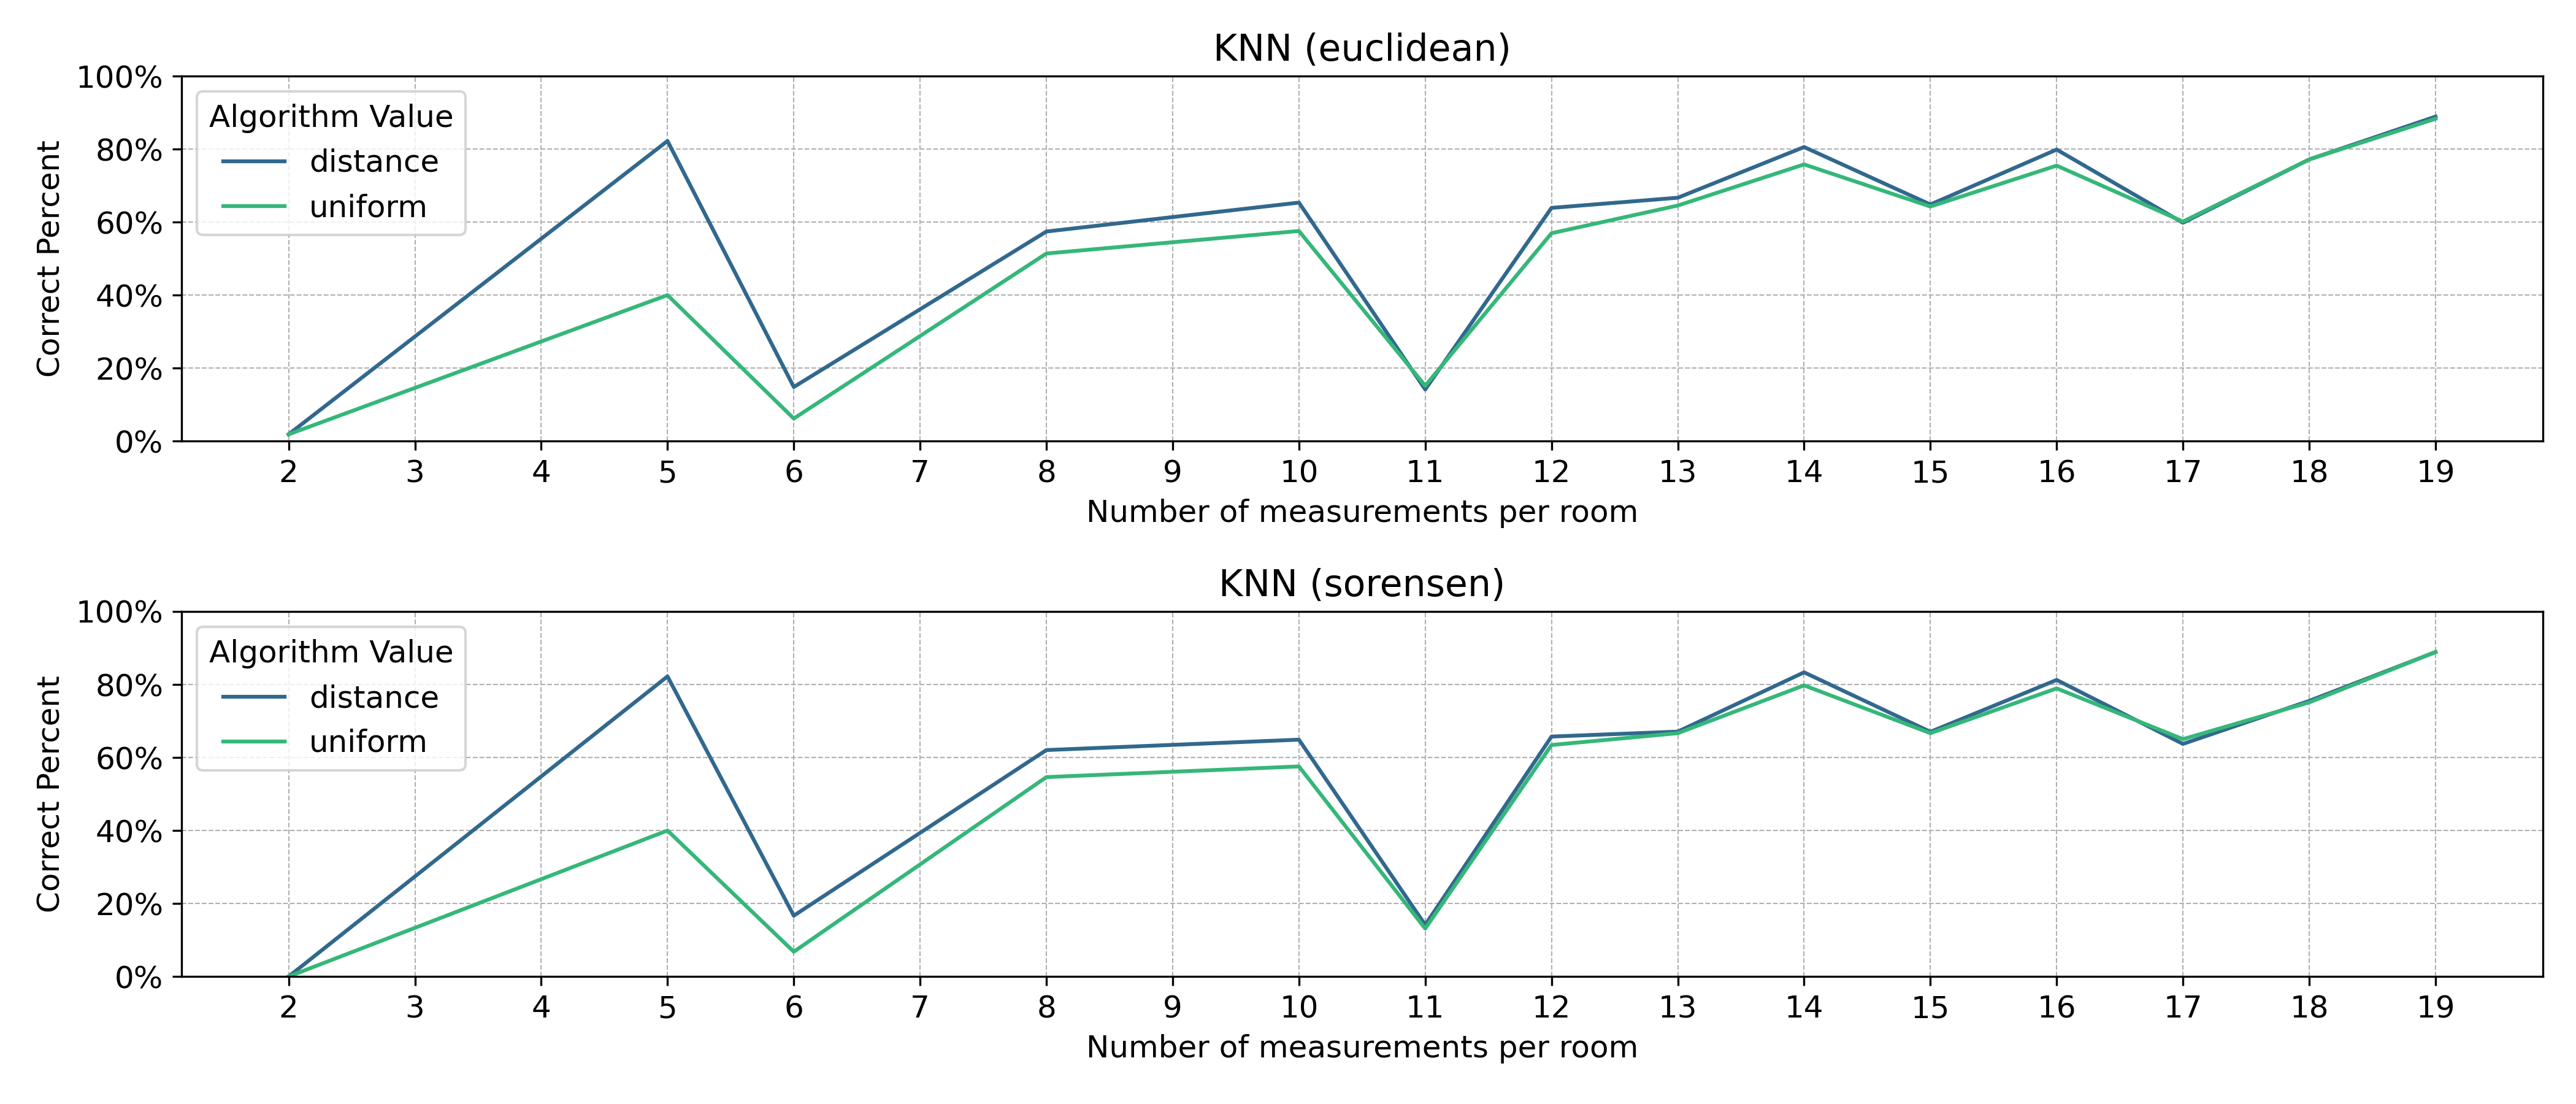
\includegraphics[width=0.8\textwidth]{images/1_distance_uniform_weights_01.png}
    \caption{Distance vs. Uniform weights}
    \label{fig:1_distance_uniform_weights_01}
\end{figure}

Ergebnis: Distance ist besser als Uniform

SVM (RBF) (gamma: scale vs. auto):

\begin{figure}[H]
    \centering
    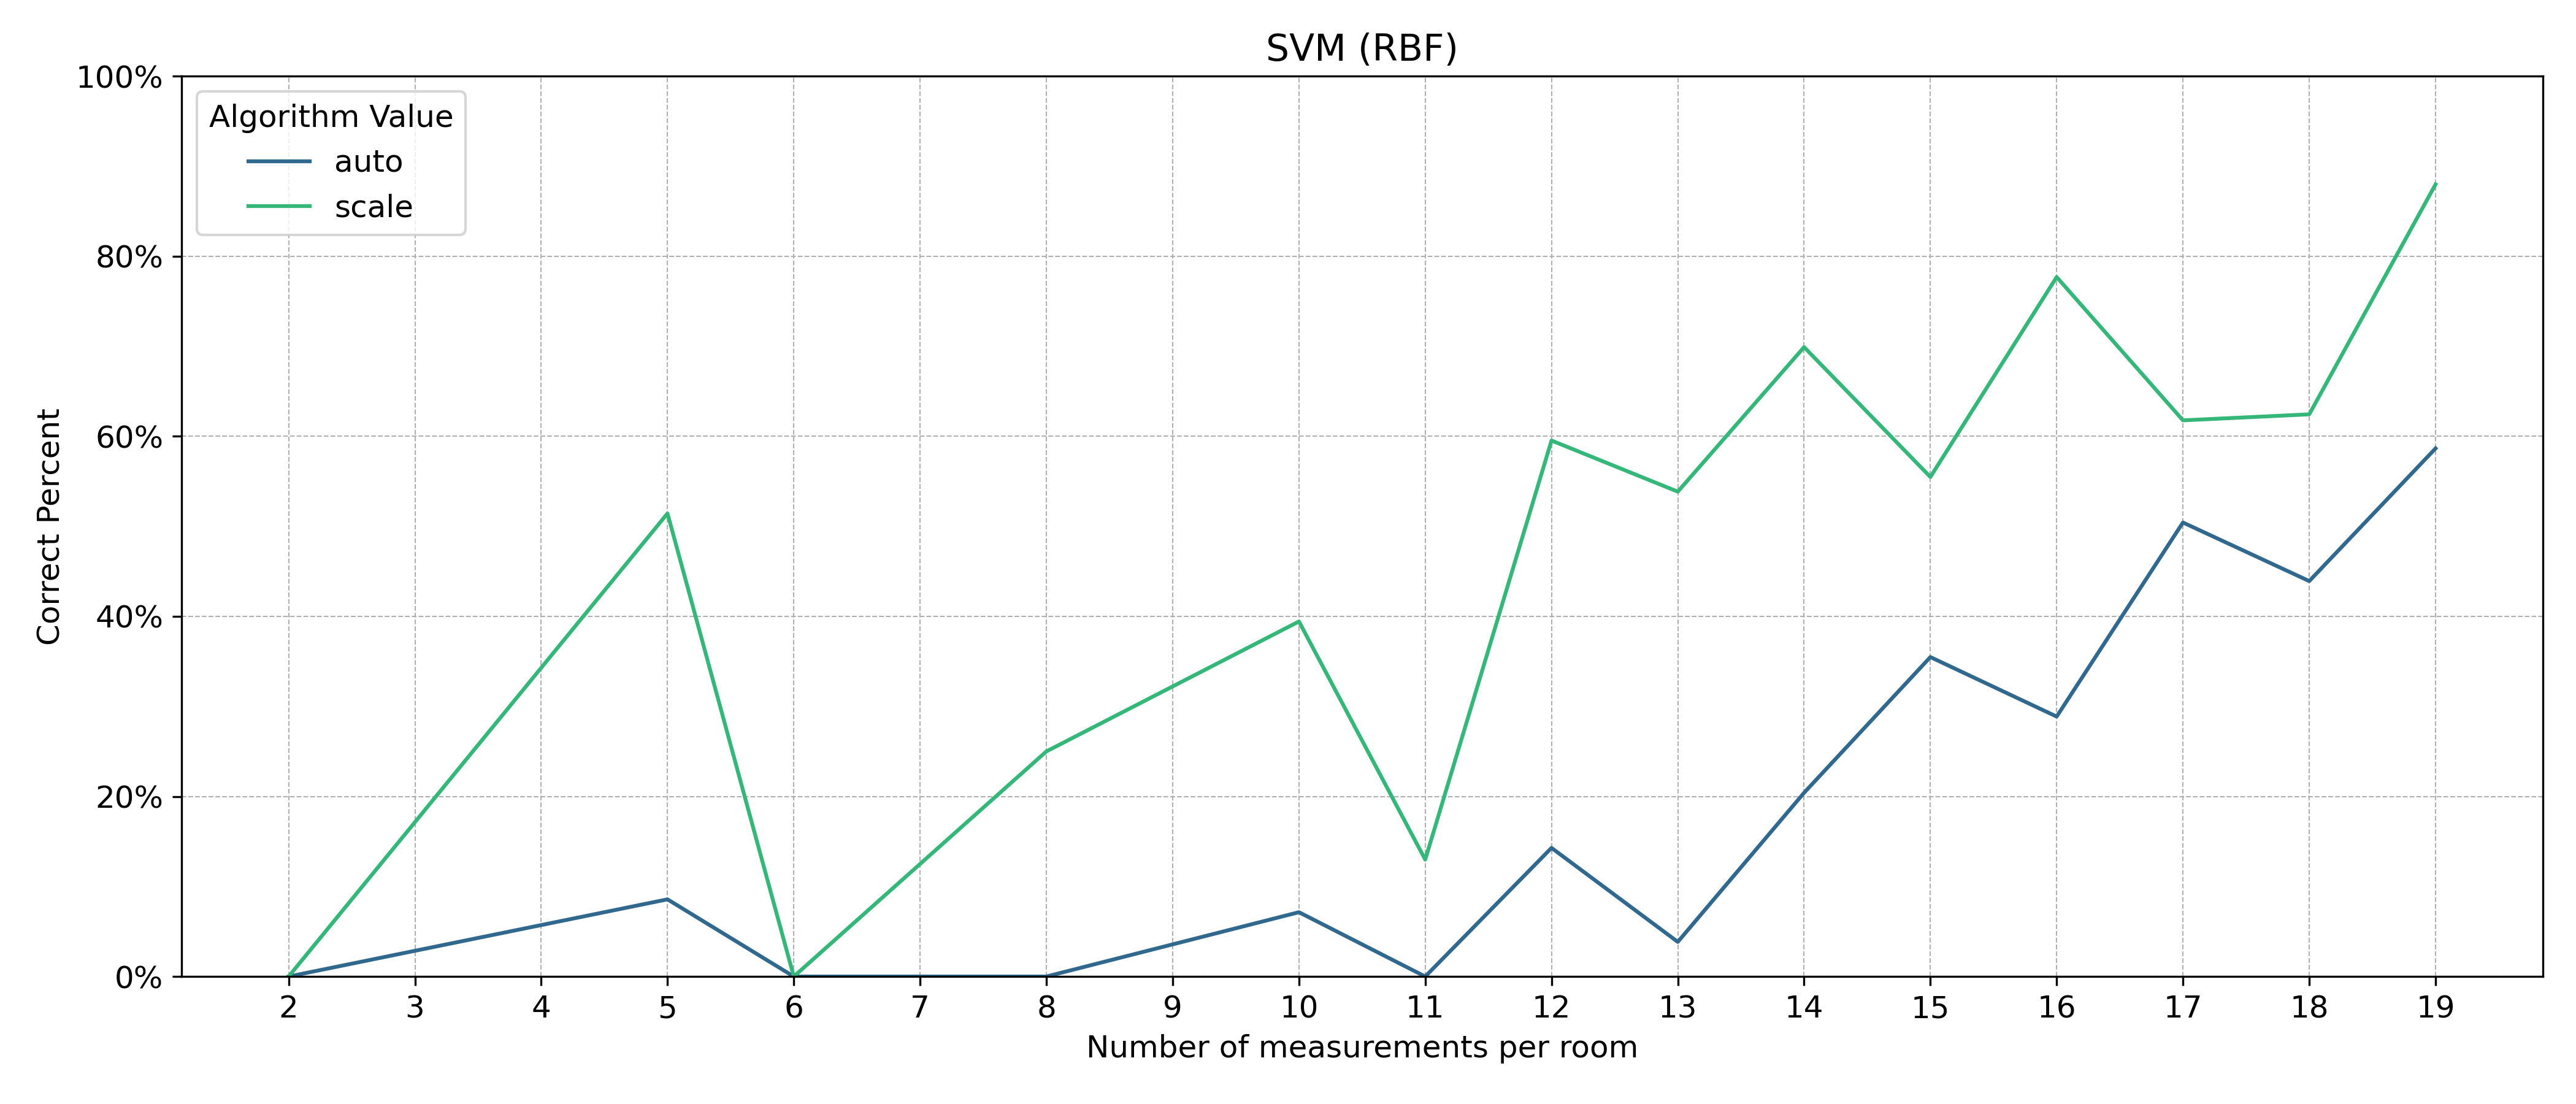
\includegraphics[width=0.8\textwidth]{images/1_best_parameters_svm_01.png}
    \caption{Scale vs. Auto bei SVM RBF}
    \label{fig:1_best_parameters_svm_01}
\end{figure}

Ergebnis: Scale ist besser als Auto

TODO: In welchem Wertebereich liegen die Werte?

TODO:
\begin{itemize}
    \item Es muss auch irgendwo stehen was der average und der weighted average ist und warum beides in den Plots gezeigt wird!
\end{itemize}

In Abbildung \ref{fig:2_best_parameters_01} sind die besten Parameter für die Algorithmen in Abhängigkeit der Anzahl der Messungen dargestellt. Die Parameter wurden durch die Anwendung des Testprogramms auf die gesammelten Daten ermittelt. Die Parameter wurden so gewählt, dass die Genauigkeit der Algorithmen maximiert wurde. In Abbildung \ref{fig:2_best_parameters_02} ist die durchschnittliche Genauigkeit der Parameter dargestellt. Die Genauigkeit wurde durch die Anwendung des Testprogramms auf die gesammelten Daten ermittelt.

\begin{figure}[H]
    \centering
    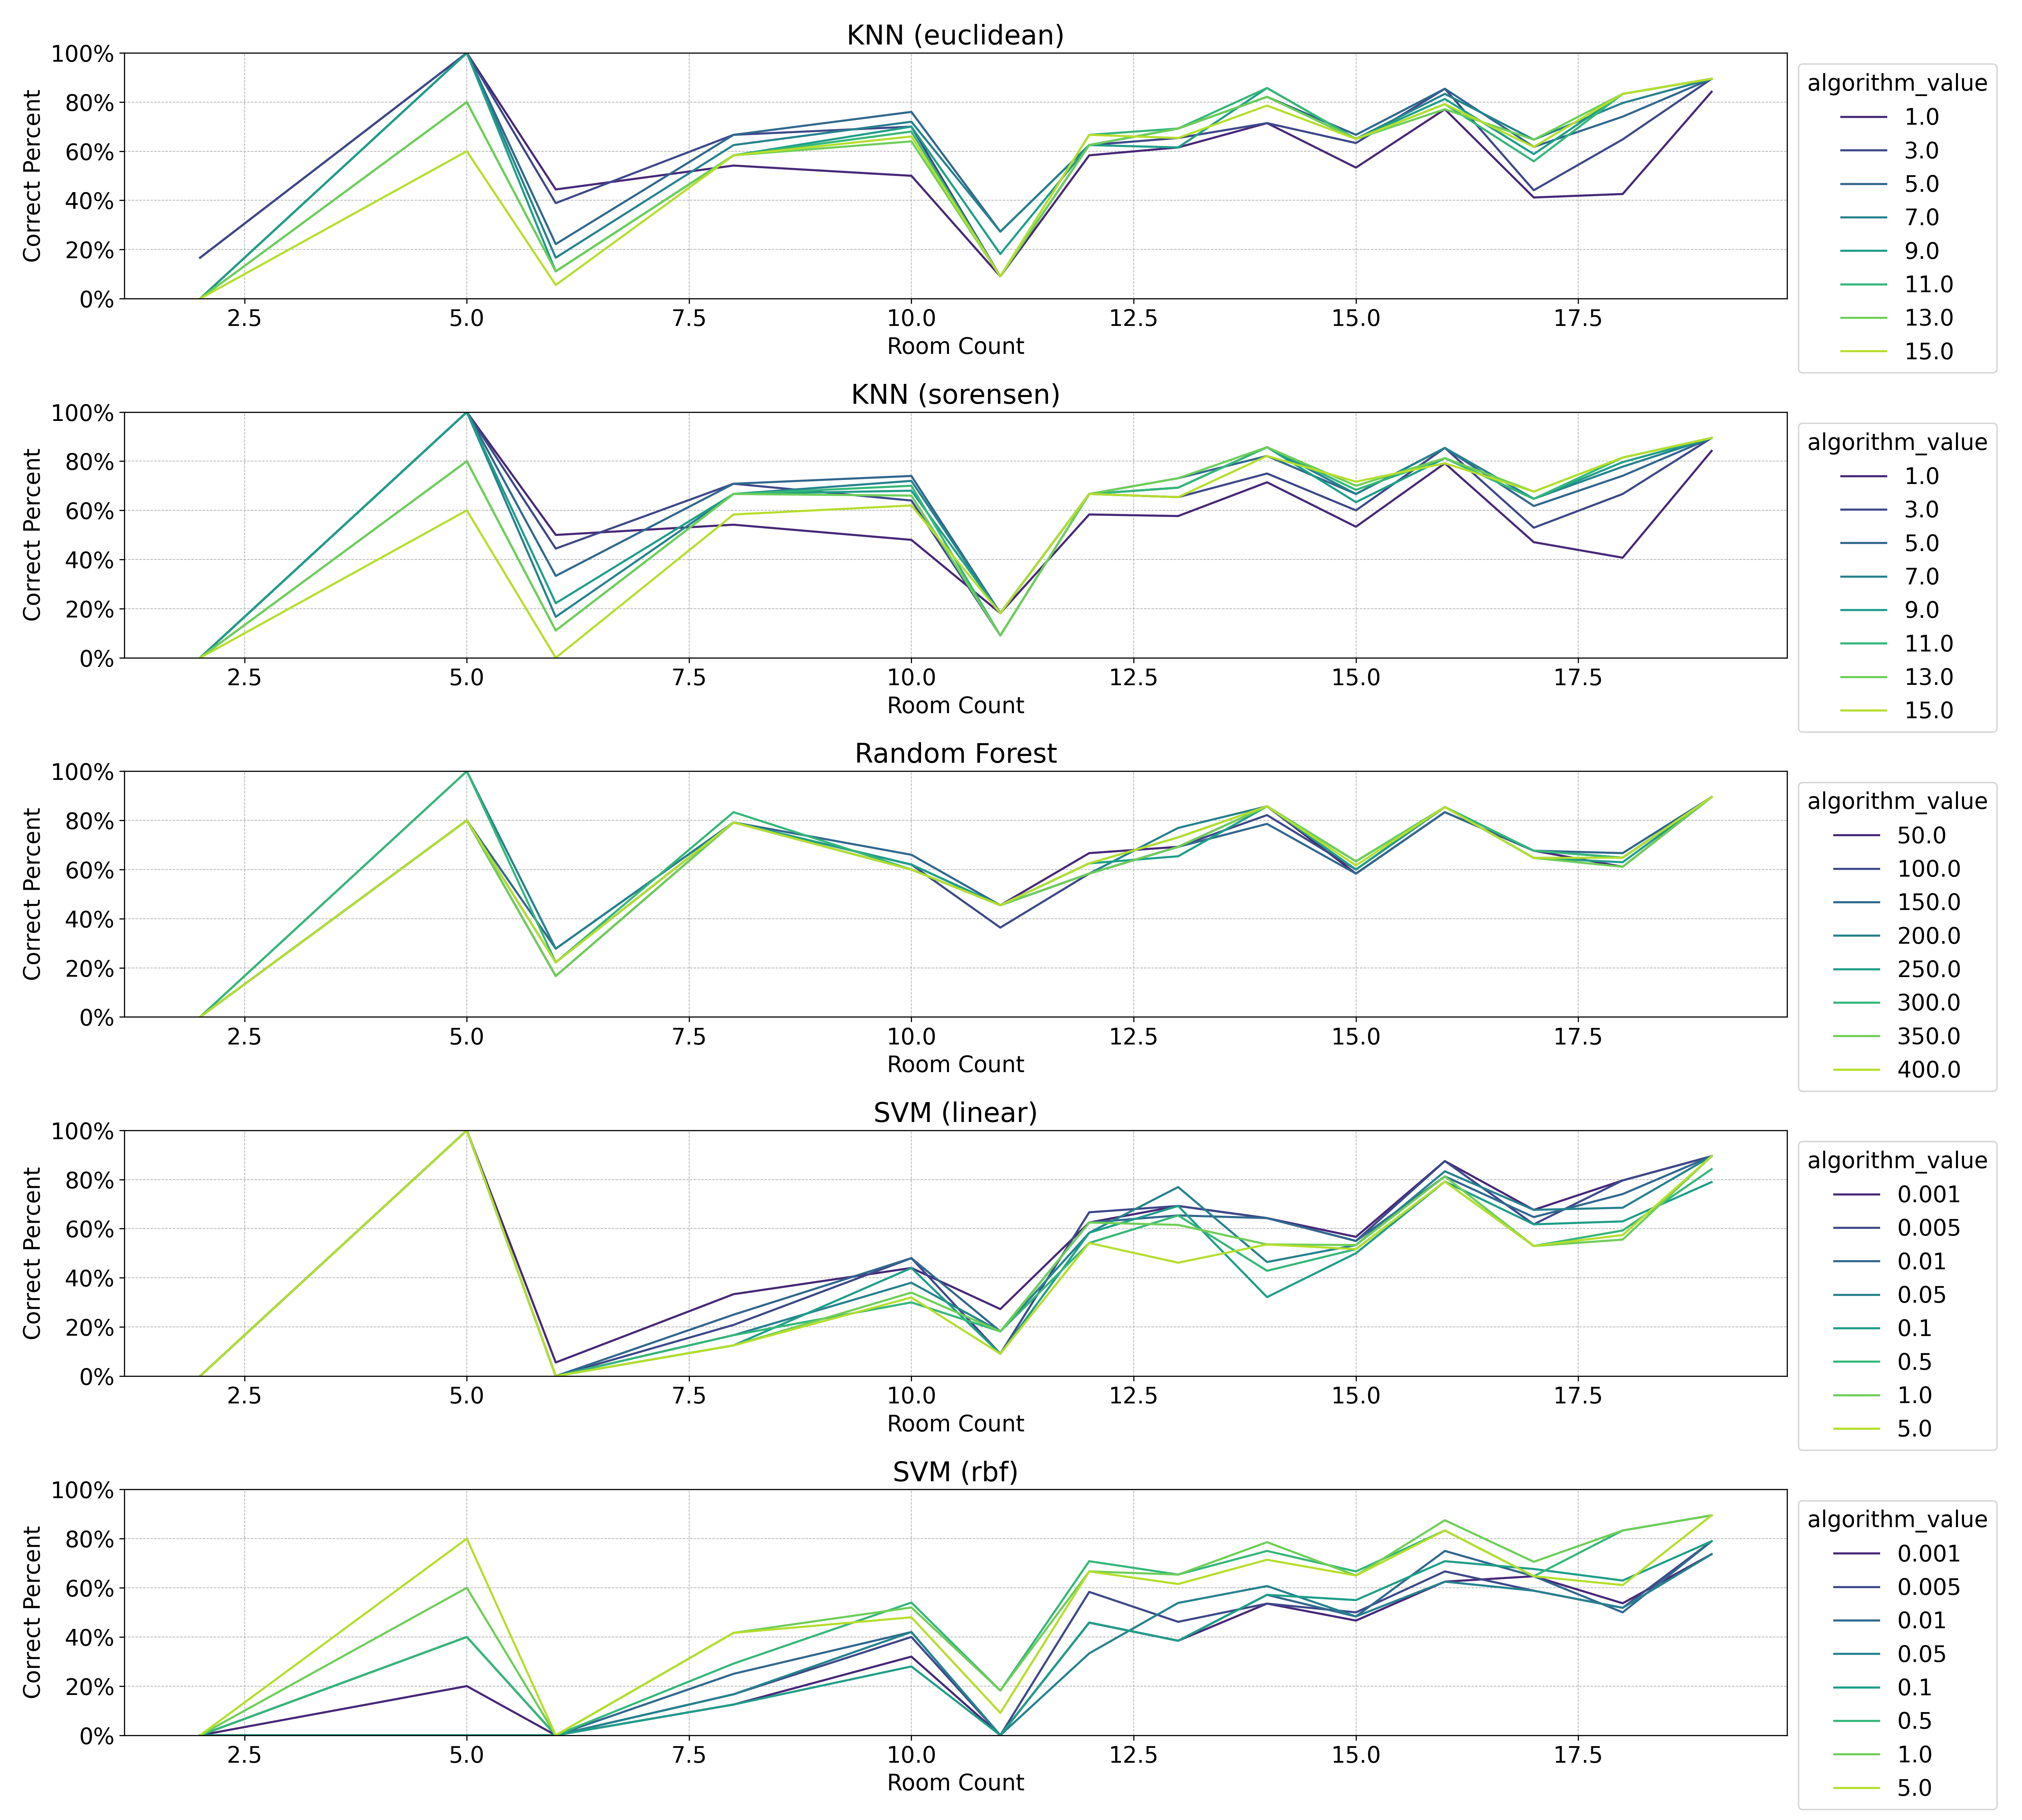
\includegraphics[width=0.8\textwidth]{images/2_best_parameters_01.png}
    \caption{Vergleich der Parameter in Abhängigkeit der Anzahl der Messungen}
    \label{fig:2_best_parameters_01}
\end{figure}

\begin{figure}[H]
    \centering
    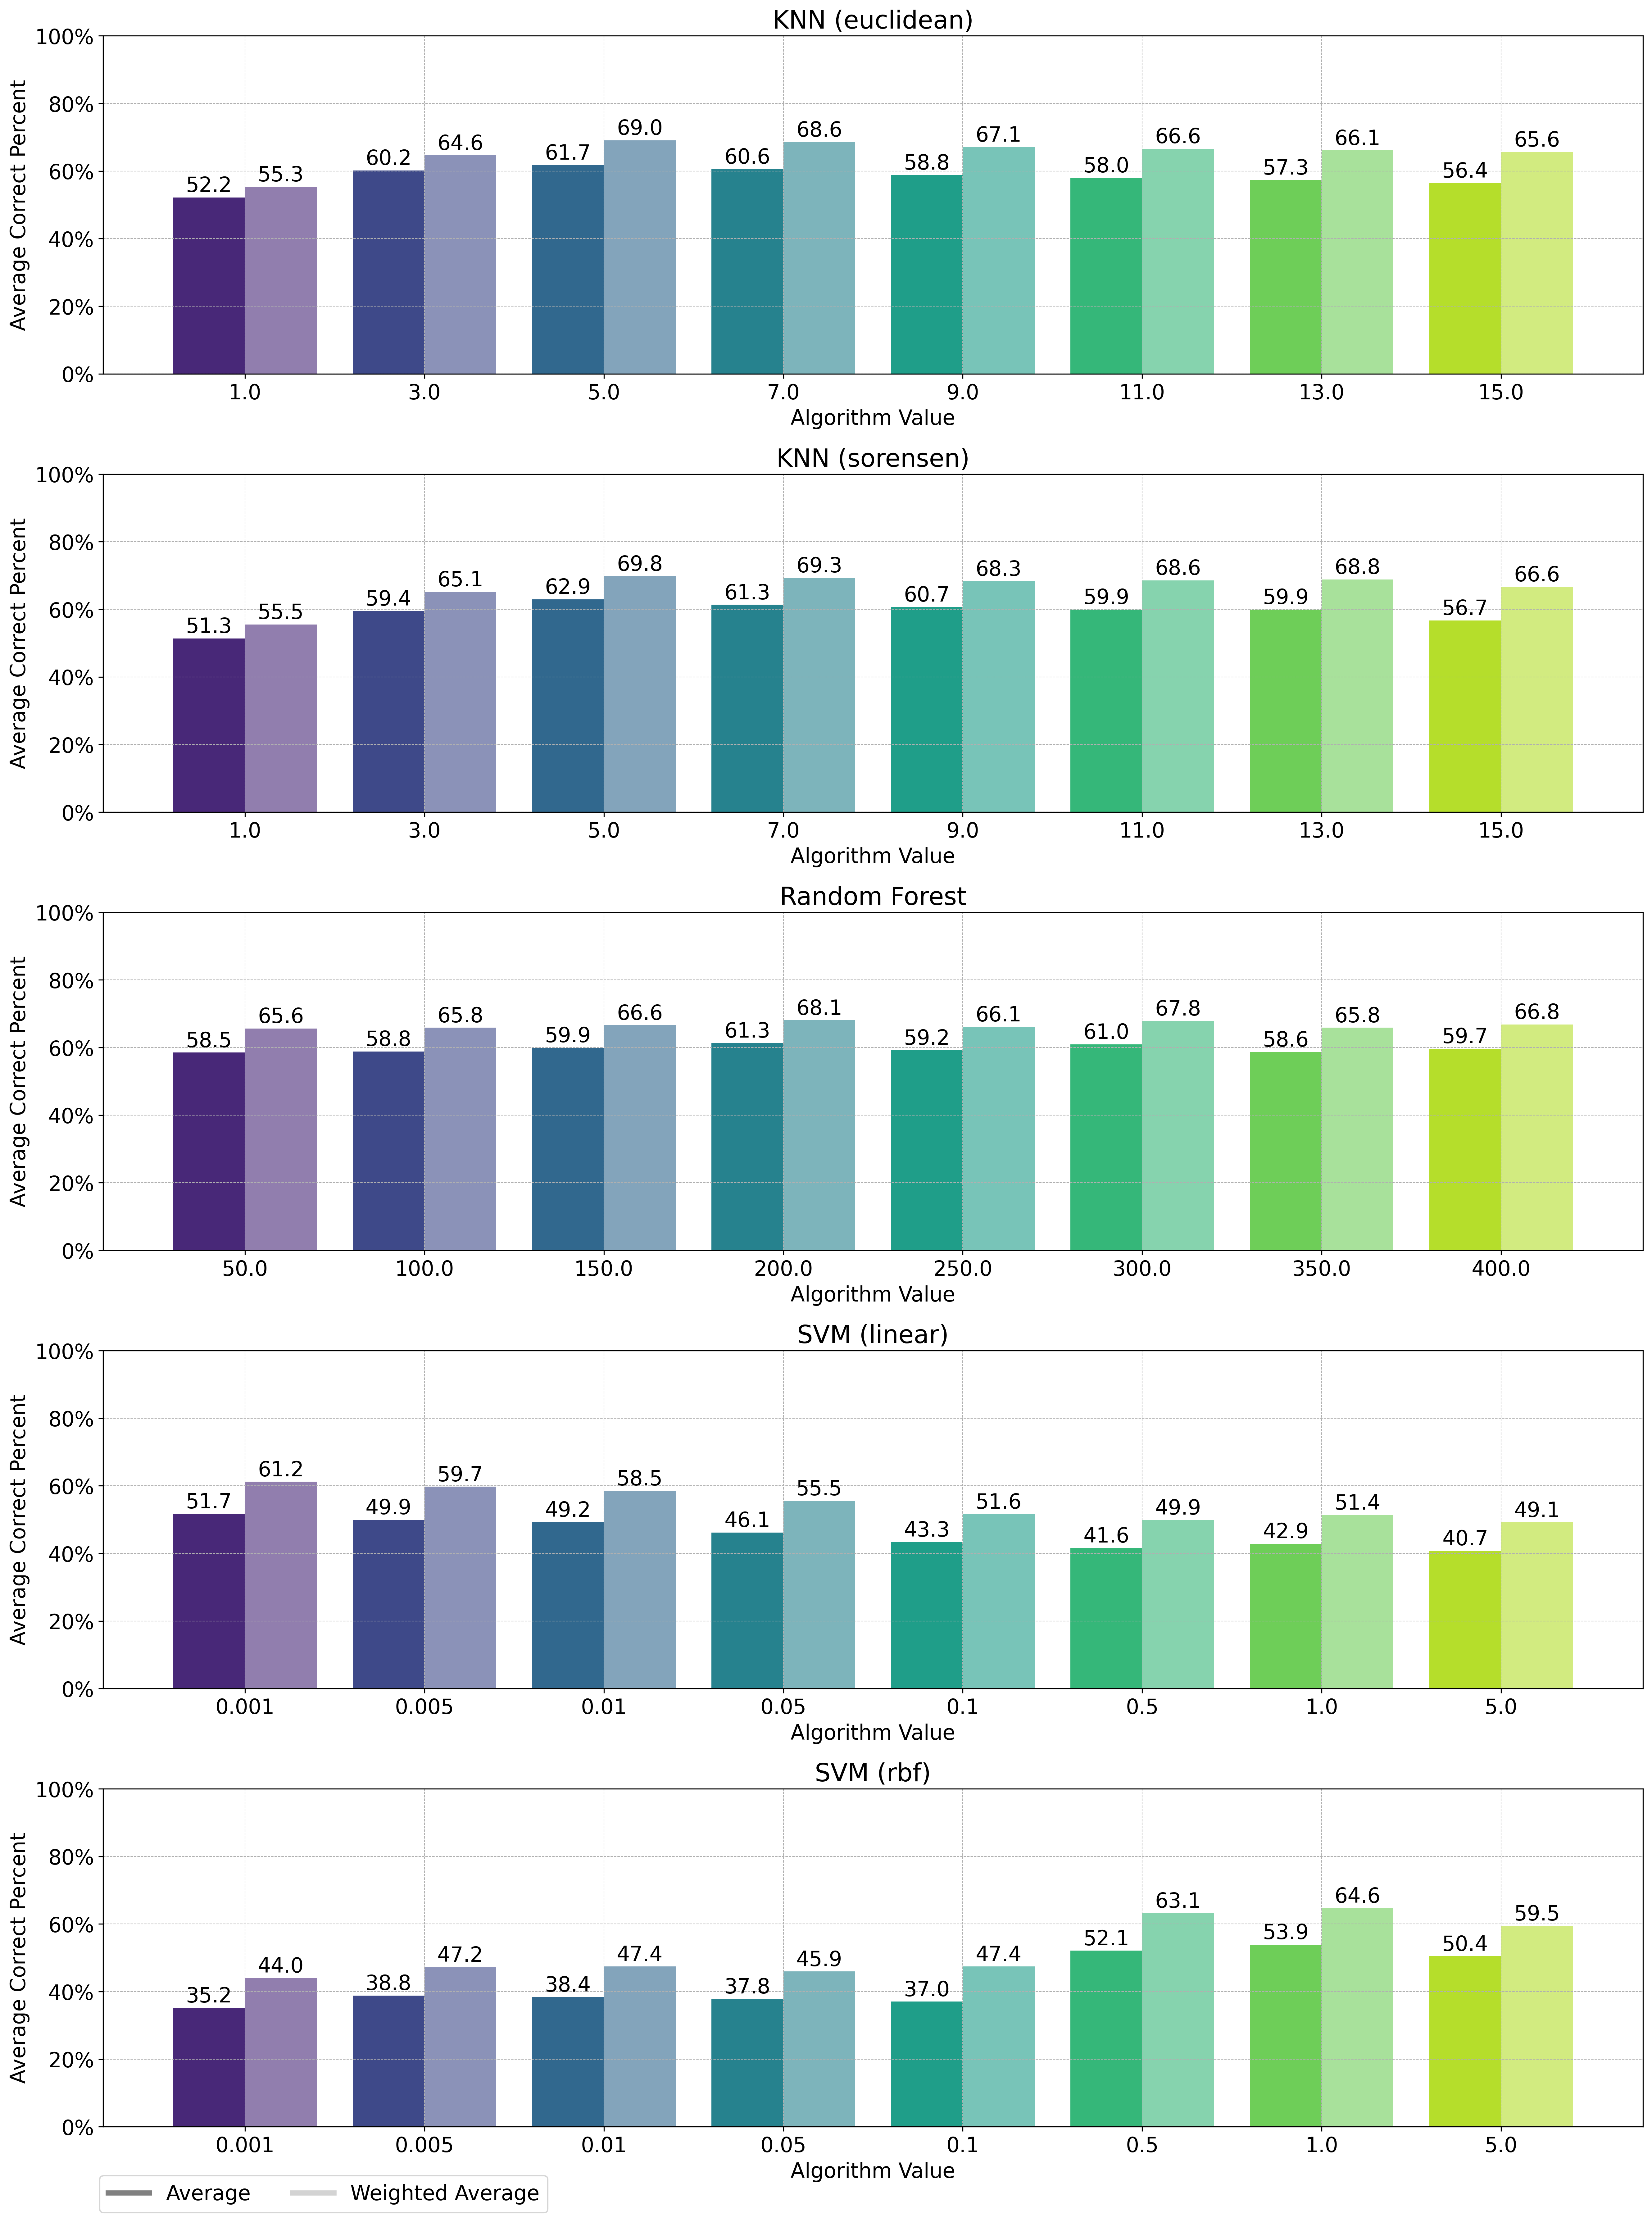
\includegraphics[width=0.8\textwidth]{images/2_best_parameters_02.png}
    \caption{Vergleich der durschnittlichen Genauigkeit der Parameter}
    \label{fig:2_best_parameters_02}
\end{figure}

Warum diese Parameter?
\begin{itemize}
    \item KNN: 1, 3, 5, 7, 9, 11, 13, 15 -> Weil ungerade (siehe Quelle bei KNN), im Wertebereich der Anzahl an Messungen pro Raum
    \item RF: 50, 100, 150, 200, 250, 300, 350, 400 Wurde gewählt, weil 407 Messpunkte existieren
    \item SVM: 0.001, 0.005, 0.01, 0.05, 0.1, 0.5, 1, 5 -> Quelle: Supervised Learning-Based Indoor Positioning System Using WiFi Fingerprints Seite 62
\end{itemize}

Ergebnisse:

\begin{itemize}
    \item KNN: 5, 7, 9
    \item RF: 100, 200, 300
    \item SVM (RBF): 0.5, 1, 5
    \item SVM (Linear): 0.001, 0.005, 0.01
\end{itemize}

\paragraph{KNN}
% \linebreak

Bei der KNN-Analyse wurden die Werte 5, 7 und 9 für k ausgewählt. Wie in Abbildung \ref{fig:2_best_parameters_01} zu sehen ist, zeigen die Genauigkeiten, dass bei Räumen mit wenigen Messungen kleinere k-Werte bessere Ergebnisse liefern, während bei Räumen mit mehr Messungen größere k-Werte vorteilhafter sind. Diese Tendenz ist sowohl bei der euclidean- als auch bei der sorensen-Metrik zu beobachten.


Abbildung \ref{fig:2_best_parameters_02} zeigt, dass bei average/euclidean die Werte 3, 5 und 7 die besten Ergebnisse liefern, während bei weighted average/euclidean die Werte 5, 7 und 9 am besten abschneiden. Bei average/sorensen erzielen die Werte 5, 7 und 9 die besten Ergebnisse, und bei weighted average/sorensen sind es die Werte 5, 7 und 13, wobei die Genauigkeit bei k = 9 und k = 11 kaum von der Genauigkeit bei k = 13 abweicht.

Generell ist die Genauigkeit bei mehreren Messungen pro Raum weniger stark von k abhängig als bei wenigen Messungen pro Raum, mit Ausnahme von sehr kleinen k-Werten wie 1 oder 3. Daher wurden für die weiteren Analysen die k-Werte 5, 7 und 9 gewählt.

\paragraph{Random Forest}
% \linebreak

Wie in Abbildung \ref{fig:2_best_parameters_01} zu sehen ist, hat der Wert für n\_estimators beim Random-Forest-Algorithmus keinen großen Einfluss. Aus diesem Grund wurden die Werte 100, 300 und 500 gewählt, um eine gleichmäßige Verteilung zu gewährleisten.

\paragraph{SVM (linear)}
% \linebreak


Interessanterweise wurden bei der linearen SVM unabhängig vom Parameter C alle Räume korrekt vorhergesagt. Sollte man vielleicht in Betracht ziehen, alle Räume mit nur 5 Messungen zu verwenden und den SVM-Algorithmus anzuwenden? Die Ursache könnte Zufall sein (weniger Messungen führen zu größerer Streuung) oder der Algorithmus ist tatsächlich so gut. Ansonsten nimmt die Genauigkeit mit zunehmendem Wert für C ab. Die besten Werte bei average und weighted average wurden für die Werte 0,001, 0,005 und 0,01 erzielt. Daher wurden für die weitere Analyse die Werte C = 0.001, 0.005 und 0.01 gewählt.

\paragraph{SVM (rbf)}
% \linebreak

Generell lässt sich in Abbildung \ref{fig:2_best_parameters_01} erkennen, dass größere Werte für C bessere Ergebnisse liefern als kleinere. Die besten Ergebnisse konnten bei average und weighted average für C = 1.0 erzielt werden. Daher wurden für die weitere Analyse die Werte C = 0.5, 1.0 und 5.0 gewählt.

\subsection{Strategien zum Umgang mit fehlenden Werten}

In Abbildung \ref{fig:3_handle_missing_values_strategy_01} ist die Genauigkeit der Algorithmen in Abhängigkeit der Strategie zum Umgang mit fehlenden Werten dargestellt. Die Strategien wurden durch die Anwendung des Testprogramms auf die gesammelten Daten ermittelt. Die Genauigkeit wurde durch die Anwendung des Testprogramms auf die gesammelten Daten ermittelt.

\begin{figure}[H]
    \centering
    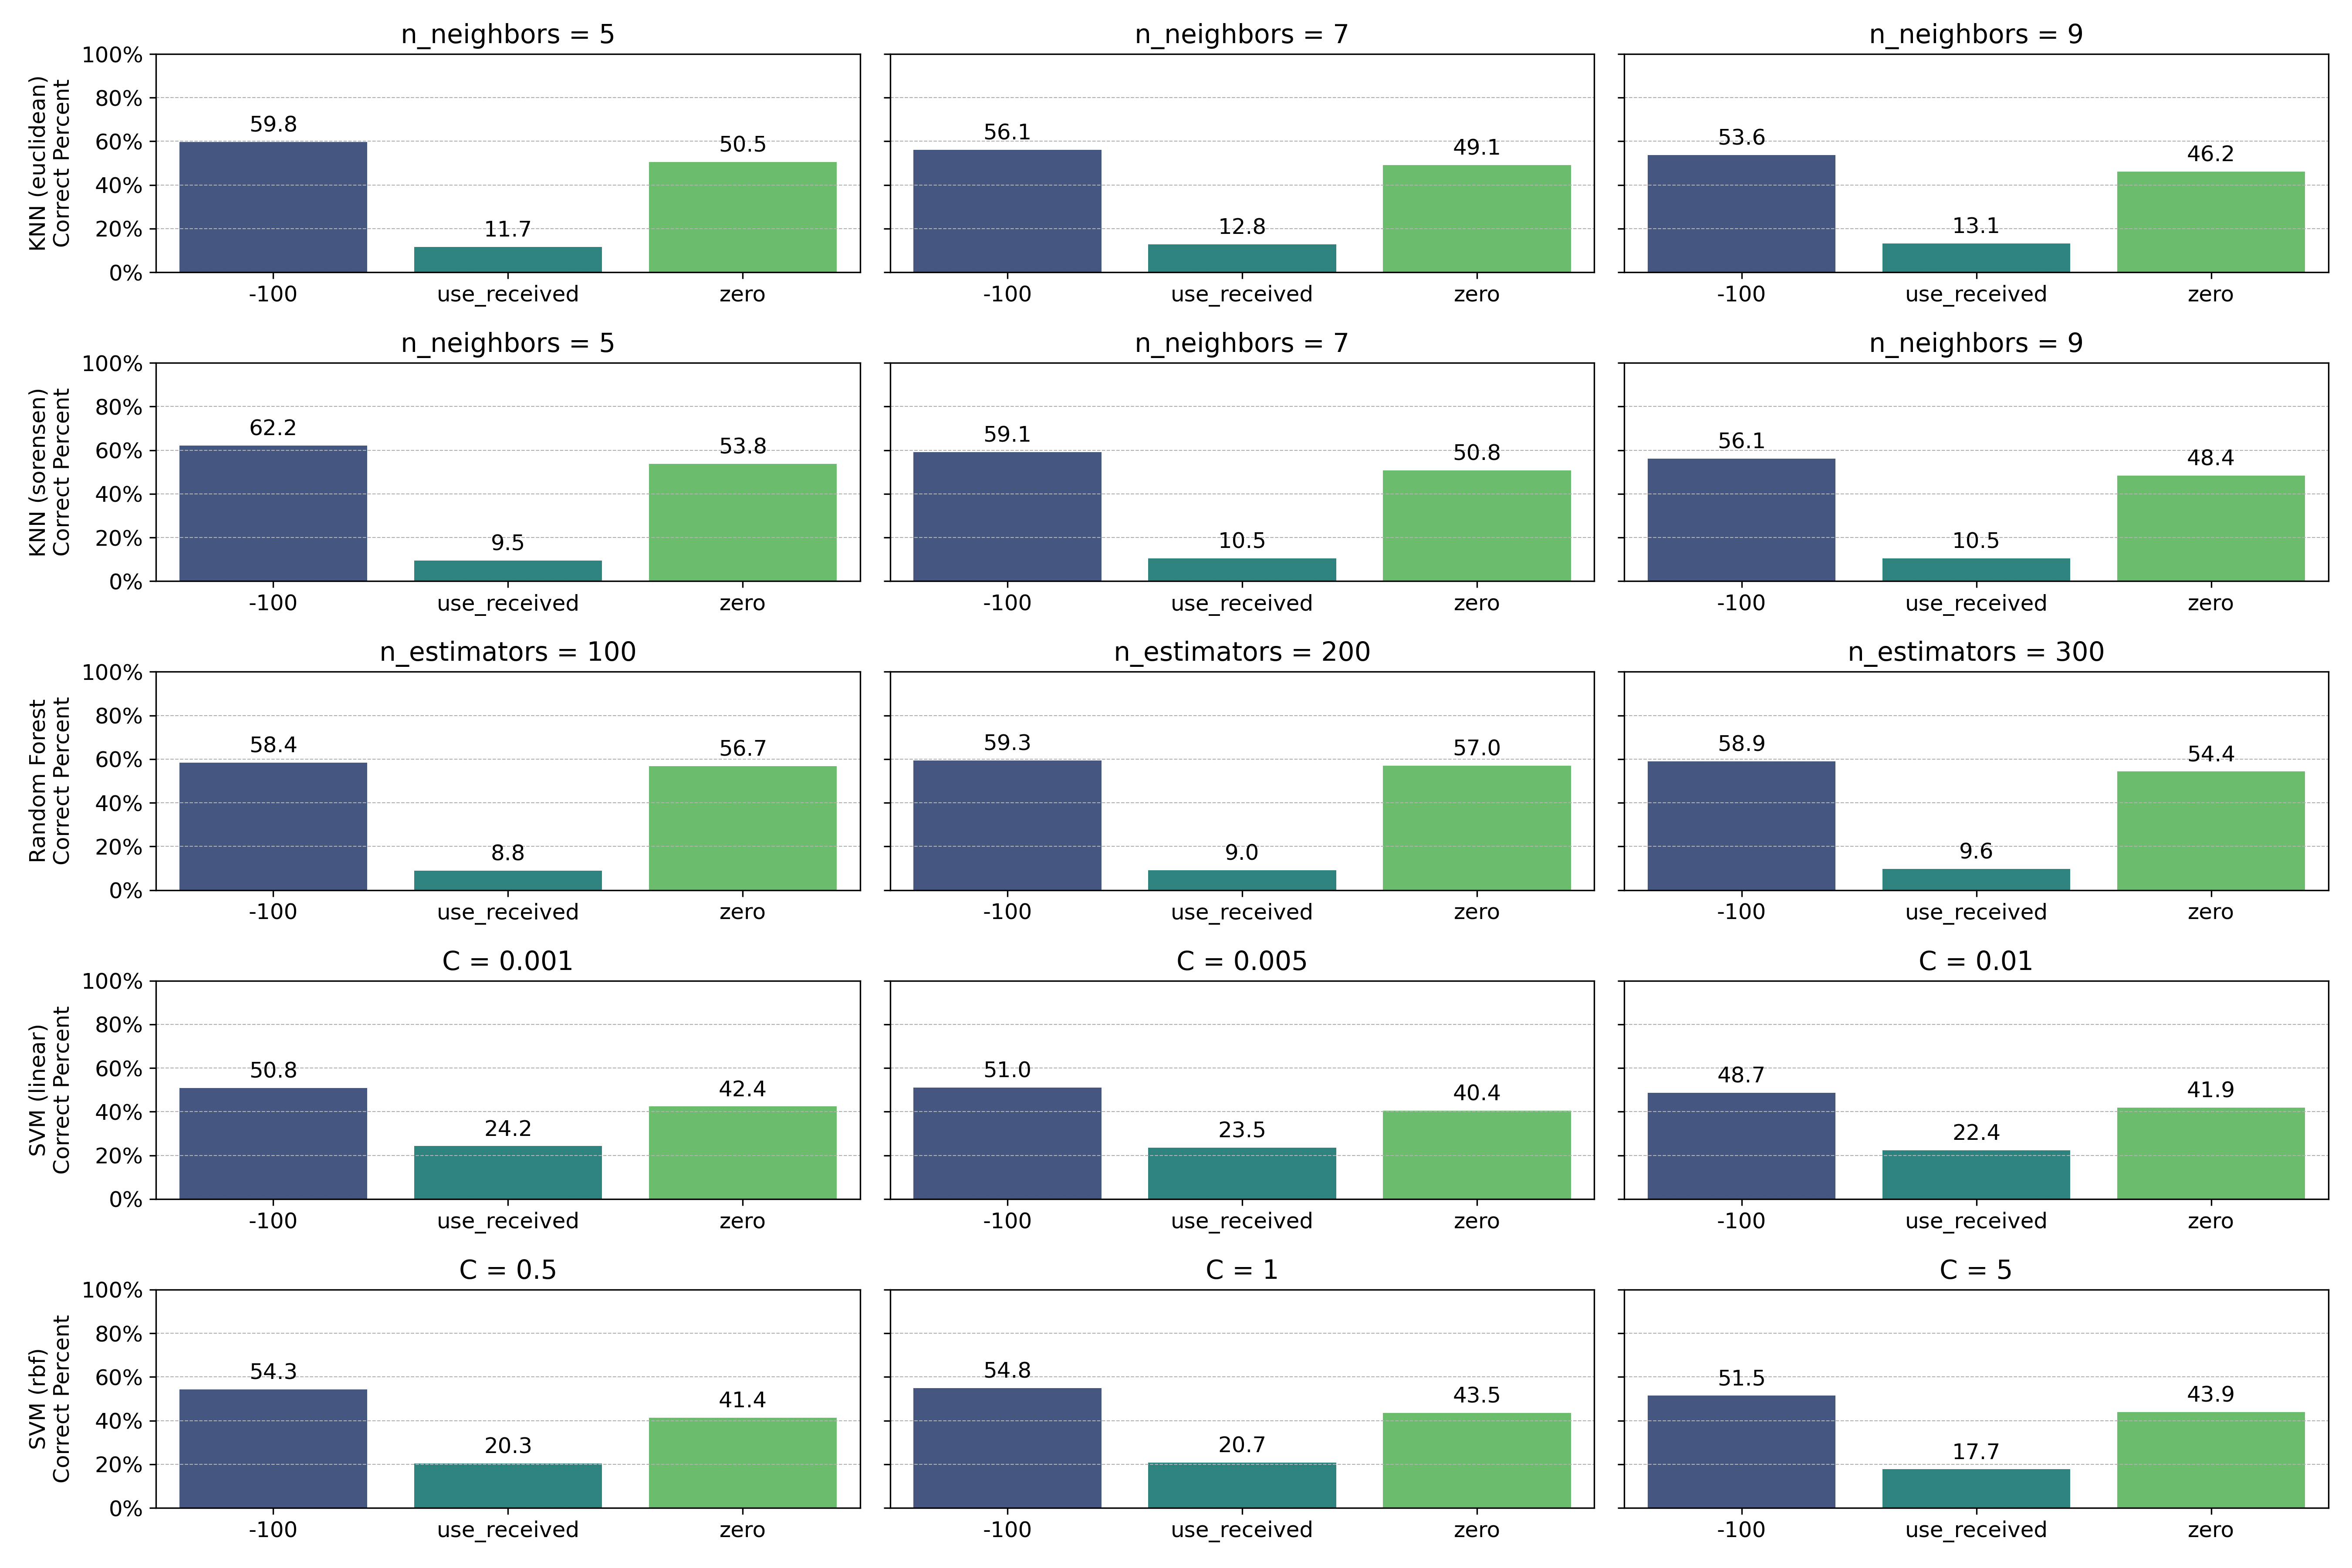
\includegraphics[width=0.8\textwidth]{images/3_handle_missing_values_strategy_01.png}
    \caption{Vergleich der Genauigkeit in Abhängigkeit der Strategie zum Umgang mit fehlenden Werten}
    \label{fig:3_handle_missing_values_strategy_01}
\end{figure}

\subsection{Einfluss der verwendeten Router}

Die Ergebnisse der verschiedenen Strategien zur Auswahl der Router sind in Abbildung \ref{fig:4_router_selection_02} dargestellt.

\begin{itemize}
    \item Alle Router sind besser als nur die eduroam Router
    \item Unterschiede nehmen mit zunehmener Anzaahl der Messungen eines Raums ab.
    \item Es wird sich trotzdem für alle Router entschieden, da die Unterschiede hauptsächlich bei wenigen Messungen auftreten und dort eine größere Streuung erwaret wird und bei den eduroam Routern sichergestellt werden kann, dass diese nicht die Position verändern
\end{itemize}

\begin{figure}[H]
    \centering
    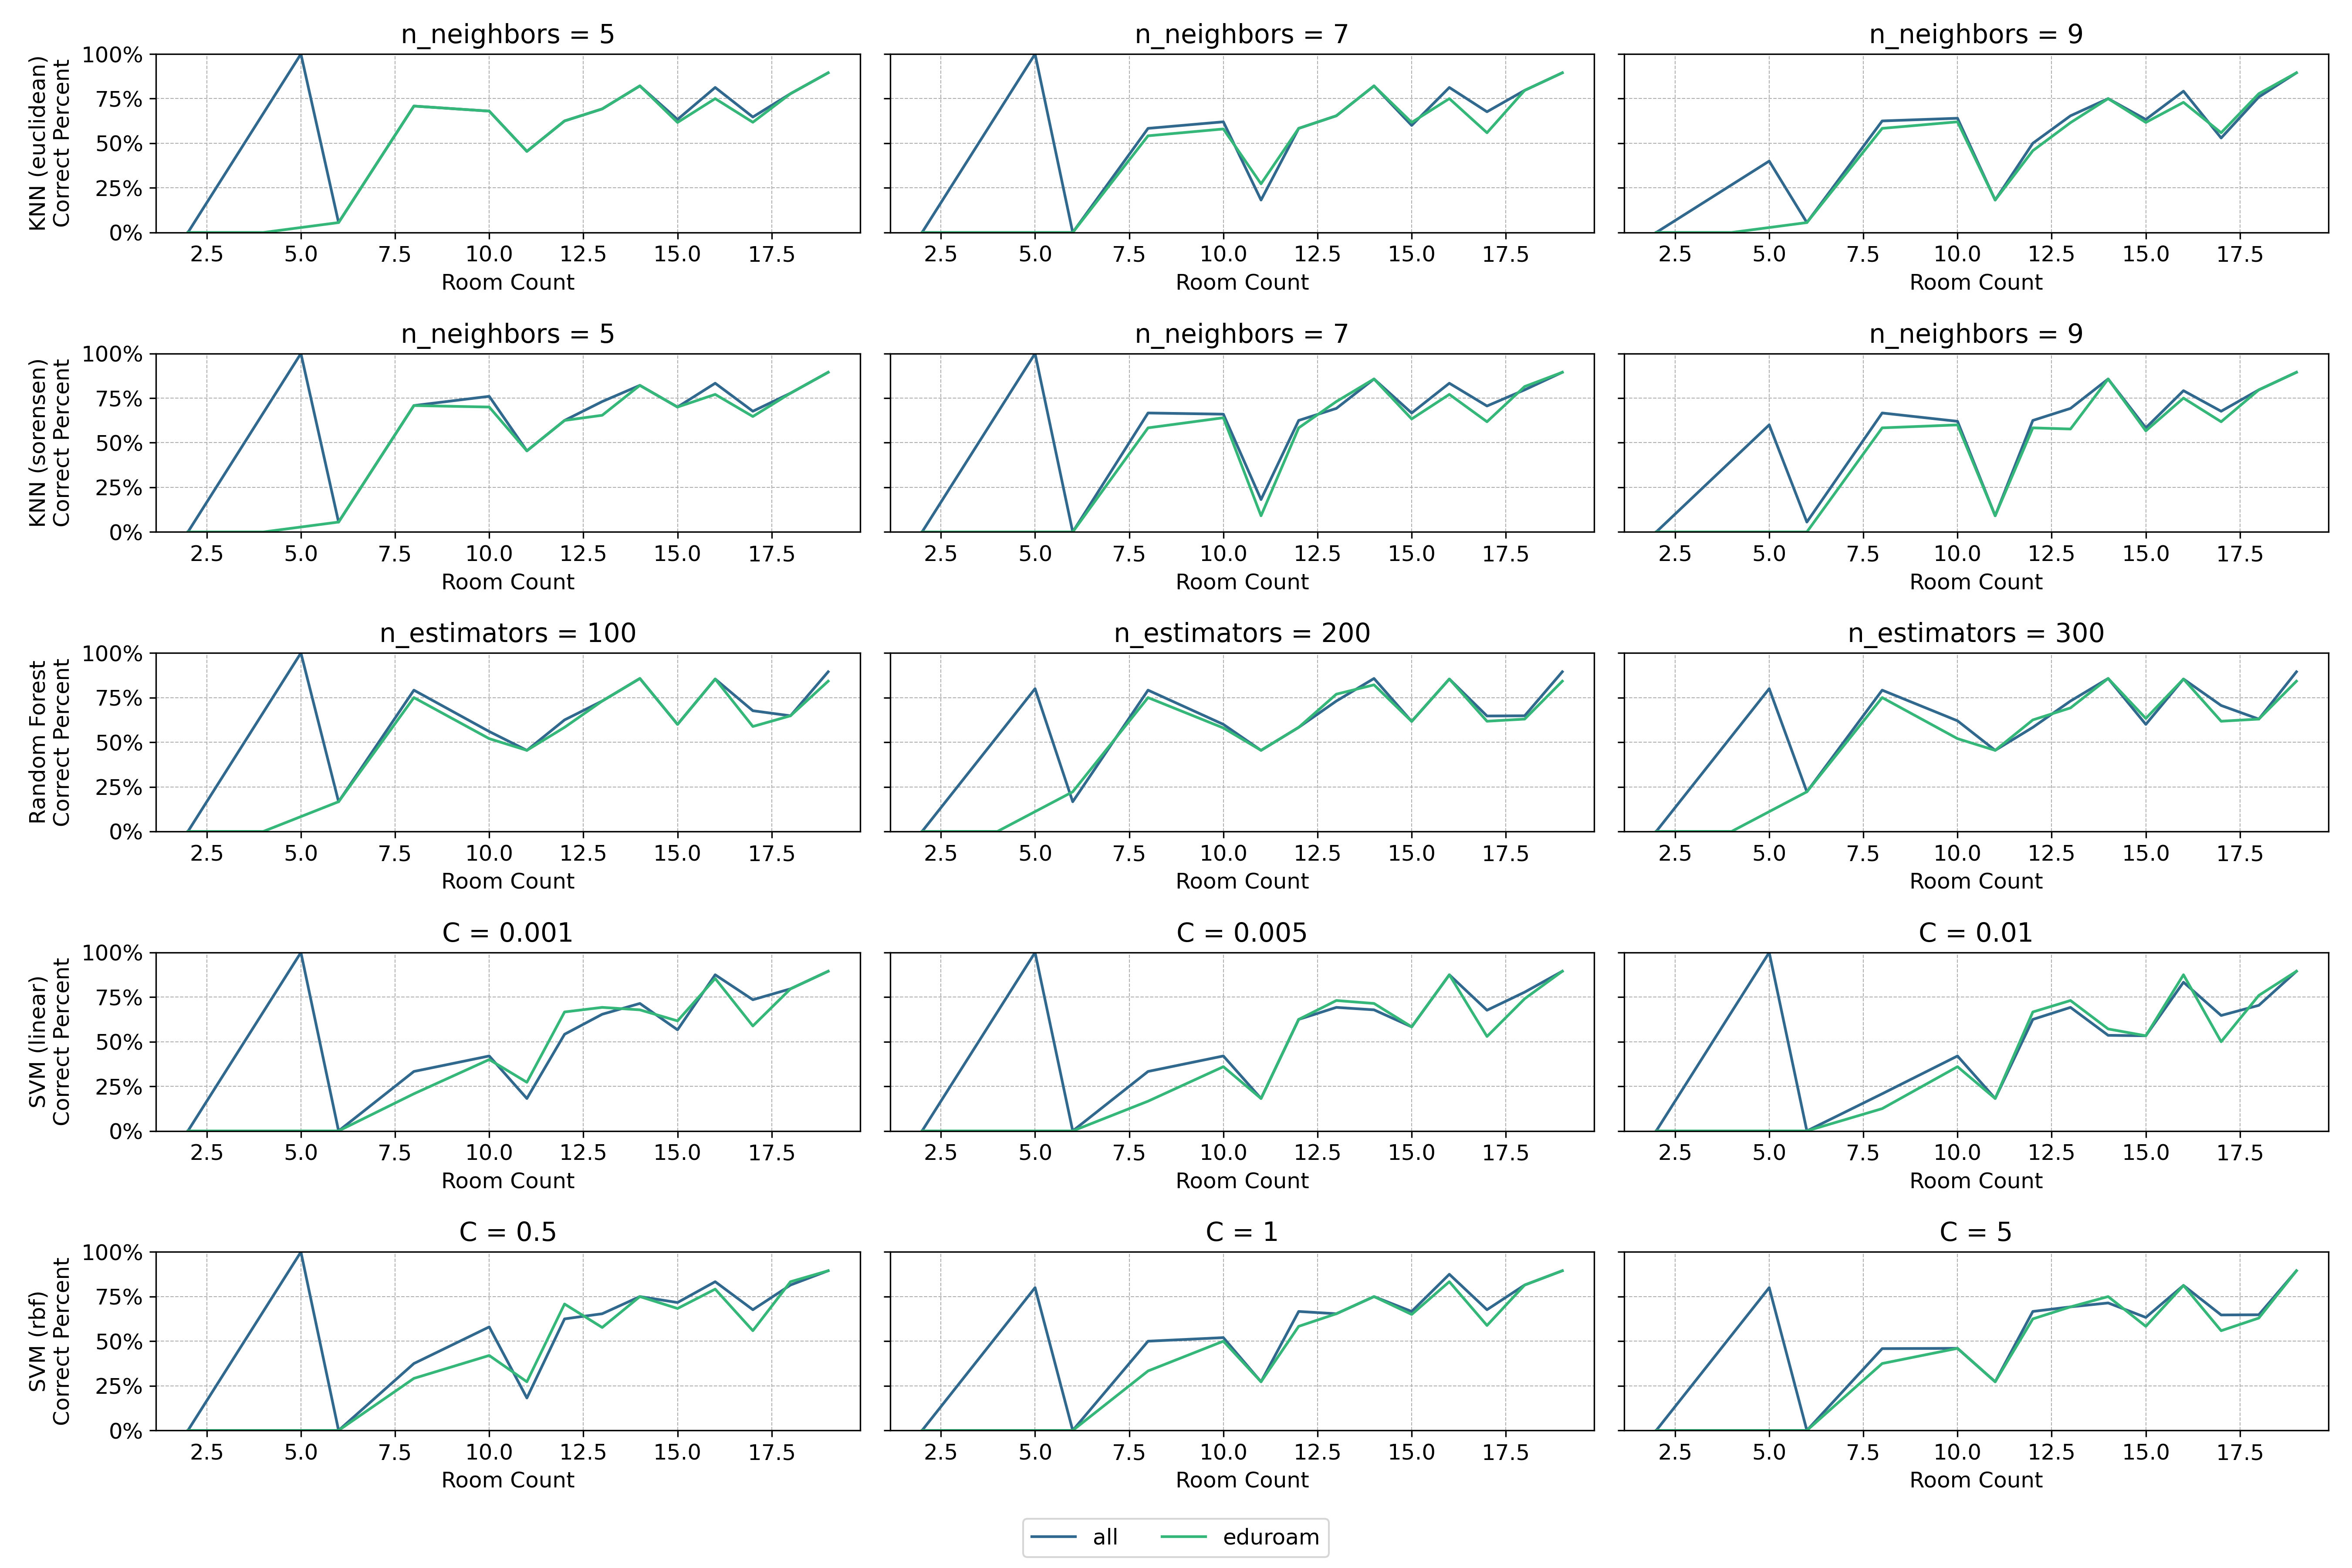
\includegraphics[width=0.8\textwidth]{images/4_router_selection_02.png}
    \caption{Auswahl der Router}
    \label{fig:4_router_selection_02}
\end{figure}

\subsection{Filterung von RSSI-Werten}
\subsubsection{Berücksichtigung nur häufig auftretender Router}

Die Ergebnisse der verschiedenen Strategien zur Auswahl des Router Presence Threshold sind in Abbildung \ref{fig:5_router_presence_threshold_02} dargestellt.

\begin{itemize}
    \item Router die in mehreren Messungen eines Raums vorhanden sind, sind aussagekräftiger als Router die nur in wenigen Messungen vorhanden sind
    \item Also: In wie viel Prozent der Messungen muss ein Router vorhanden sein, damit er berücksichtigt wird
    \item Das bedeutet, dass bei wenig Messungen die Auswirkungen gering sein sollten
\end{itemize}

\begin{itemize}
    \item bei allen Algorithmen ist 0 am besten
    \item Interessant: Bei allen Algos haben die Genauigkeiten in Abhängigkkeit der Messungen pro Raum einen ähnlichen Verlauf und sind mit zunehmendem Router Presence Threshold schlechter, AUSSER bei SVM. Doer sind bei wenigen Messungen die größeren Router Presence Thresholds besser und bei mehr Messungen die kleineren. -> Deswegen wurde hier 0.25 verwendet, da dieser Wert im Schnitt die besten Ergebnisse erzielt
    \item SVM-Kipppunkt bei 10
\end{itemize}

\begin{figure}[H]
    \centering
    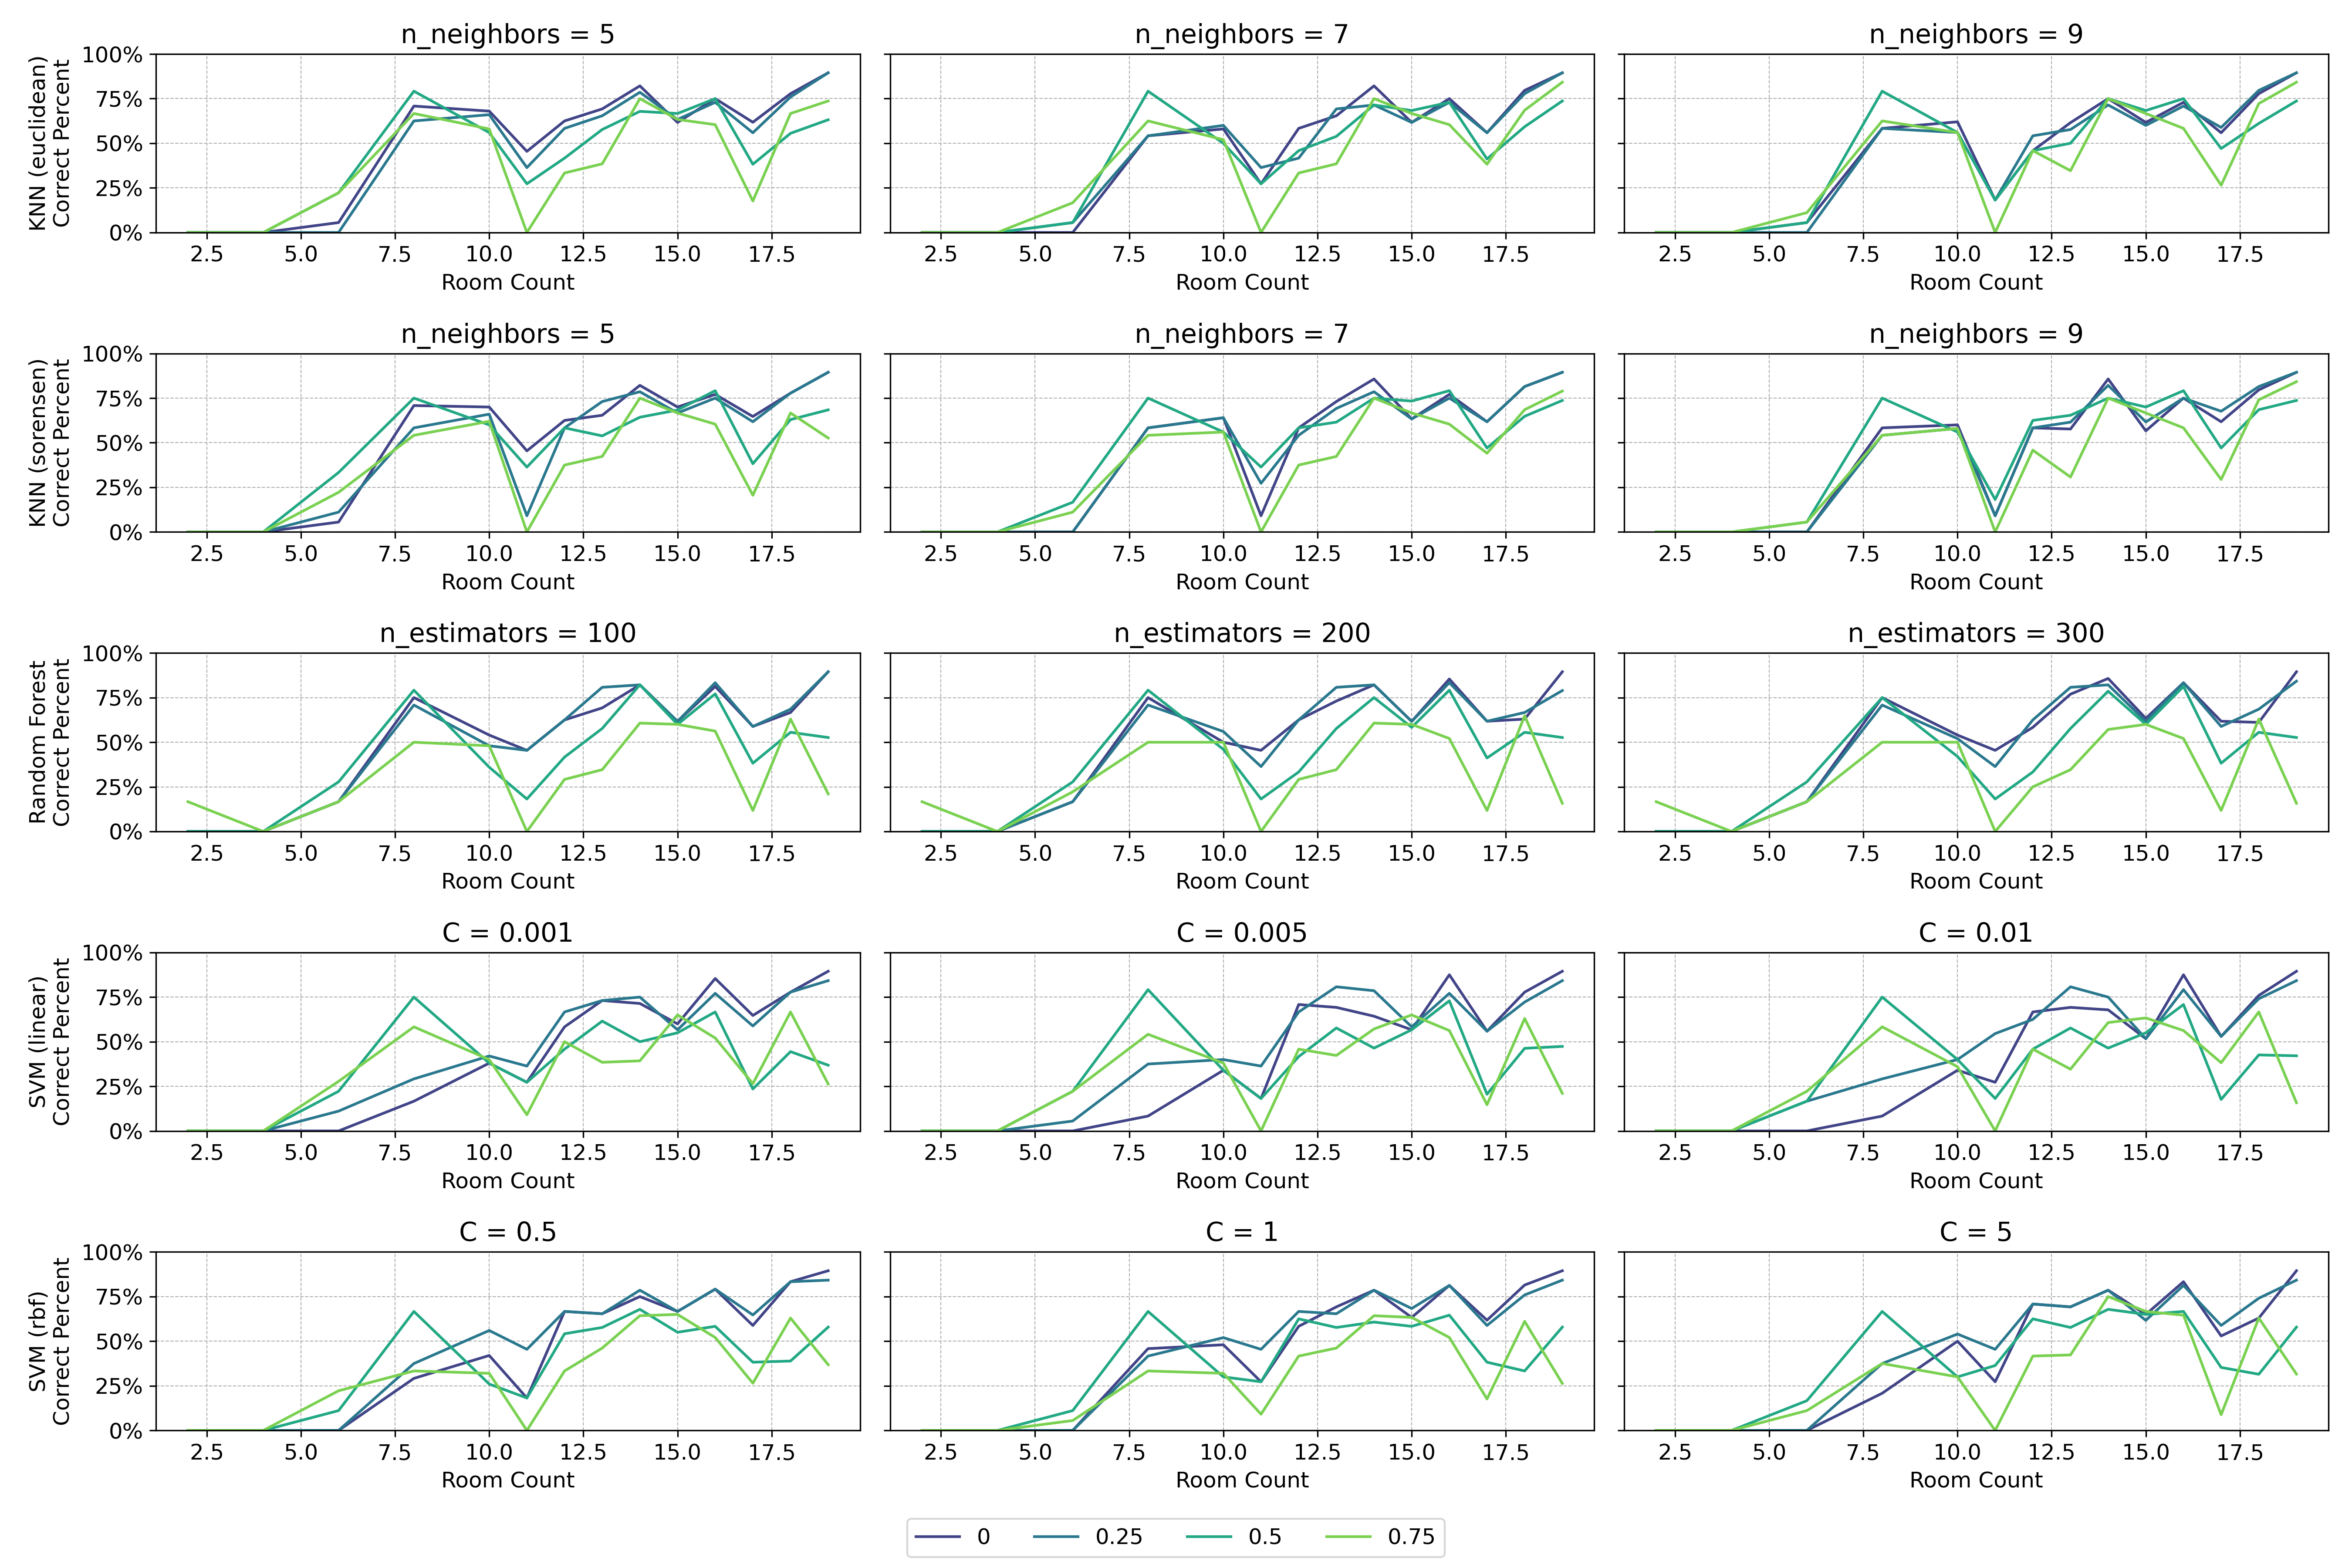
\includegraphics[width=0.8\textwidth]{images/5_router_presence_threshold_02.png}
    \caption{Vergleich der Genauigkeit in Abhängigkeit des Schwellenwerts für die Anzahl der Messungen eines Routers}
    \label{fig:5_router_presence_threshold_02}
\end{figure}

\subsubsection{Ausschluss von Routern mit schwachem Signal}

Die Ergebnisse der verschiedenen Strategien zur Auswahl des Router Rssi Threshold sind in Abbildung \ref{fig:6_router_rssi_threshold_01} dargestellt.

\begin{itemize}
    \item Idee: sehr kleine RSSI Werte werden ignoriert/so getan, als wäre die bei der Messung nicht dabei
    \item Gedanke dahiner: Router mit größeren RSSI-Werten sind aussagekräftiger und sollten dadurch mehr Einfluss haben
    \item Ergebnis: Bei allen Algorithmen ist -100 am besten -> Router mit geringen RSSI-Werten haben einen größeren Einfluss als vermutet
    \item Idee ist nicht von mir, sondern kommt aus dem Paper: Quelle: Comprehensive analysis of distance and similarity measures for Wi-Fi fingerprinting indoor positioning systems
    \item Die Thresholds sind: -100, -90, -80, -70, -60, -50, -40
\end{itemize}

\begin{figure}[H]
    \centering
    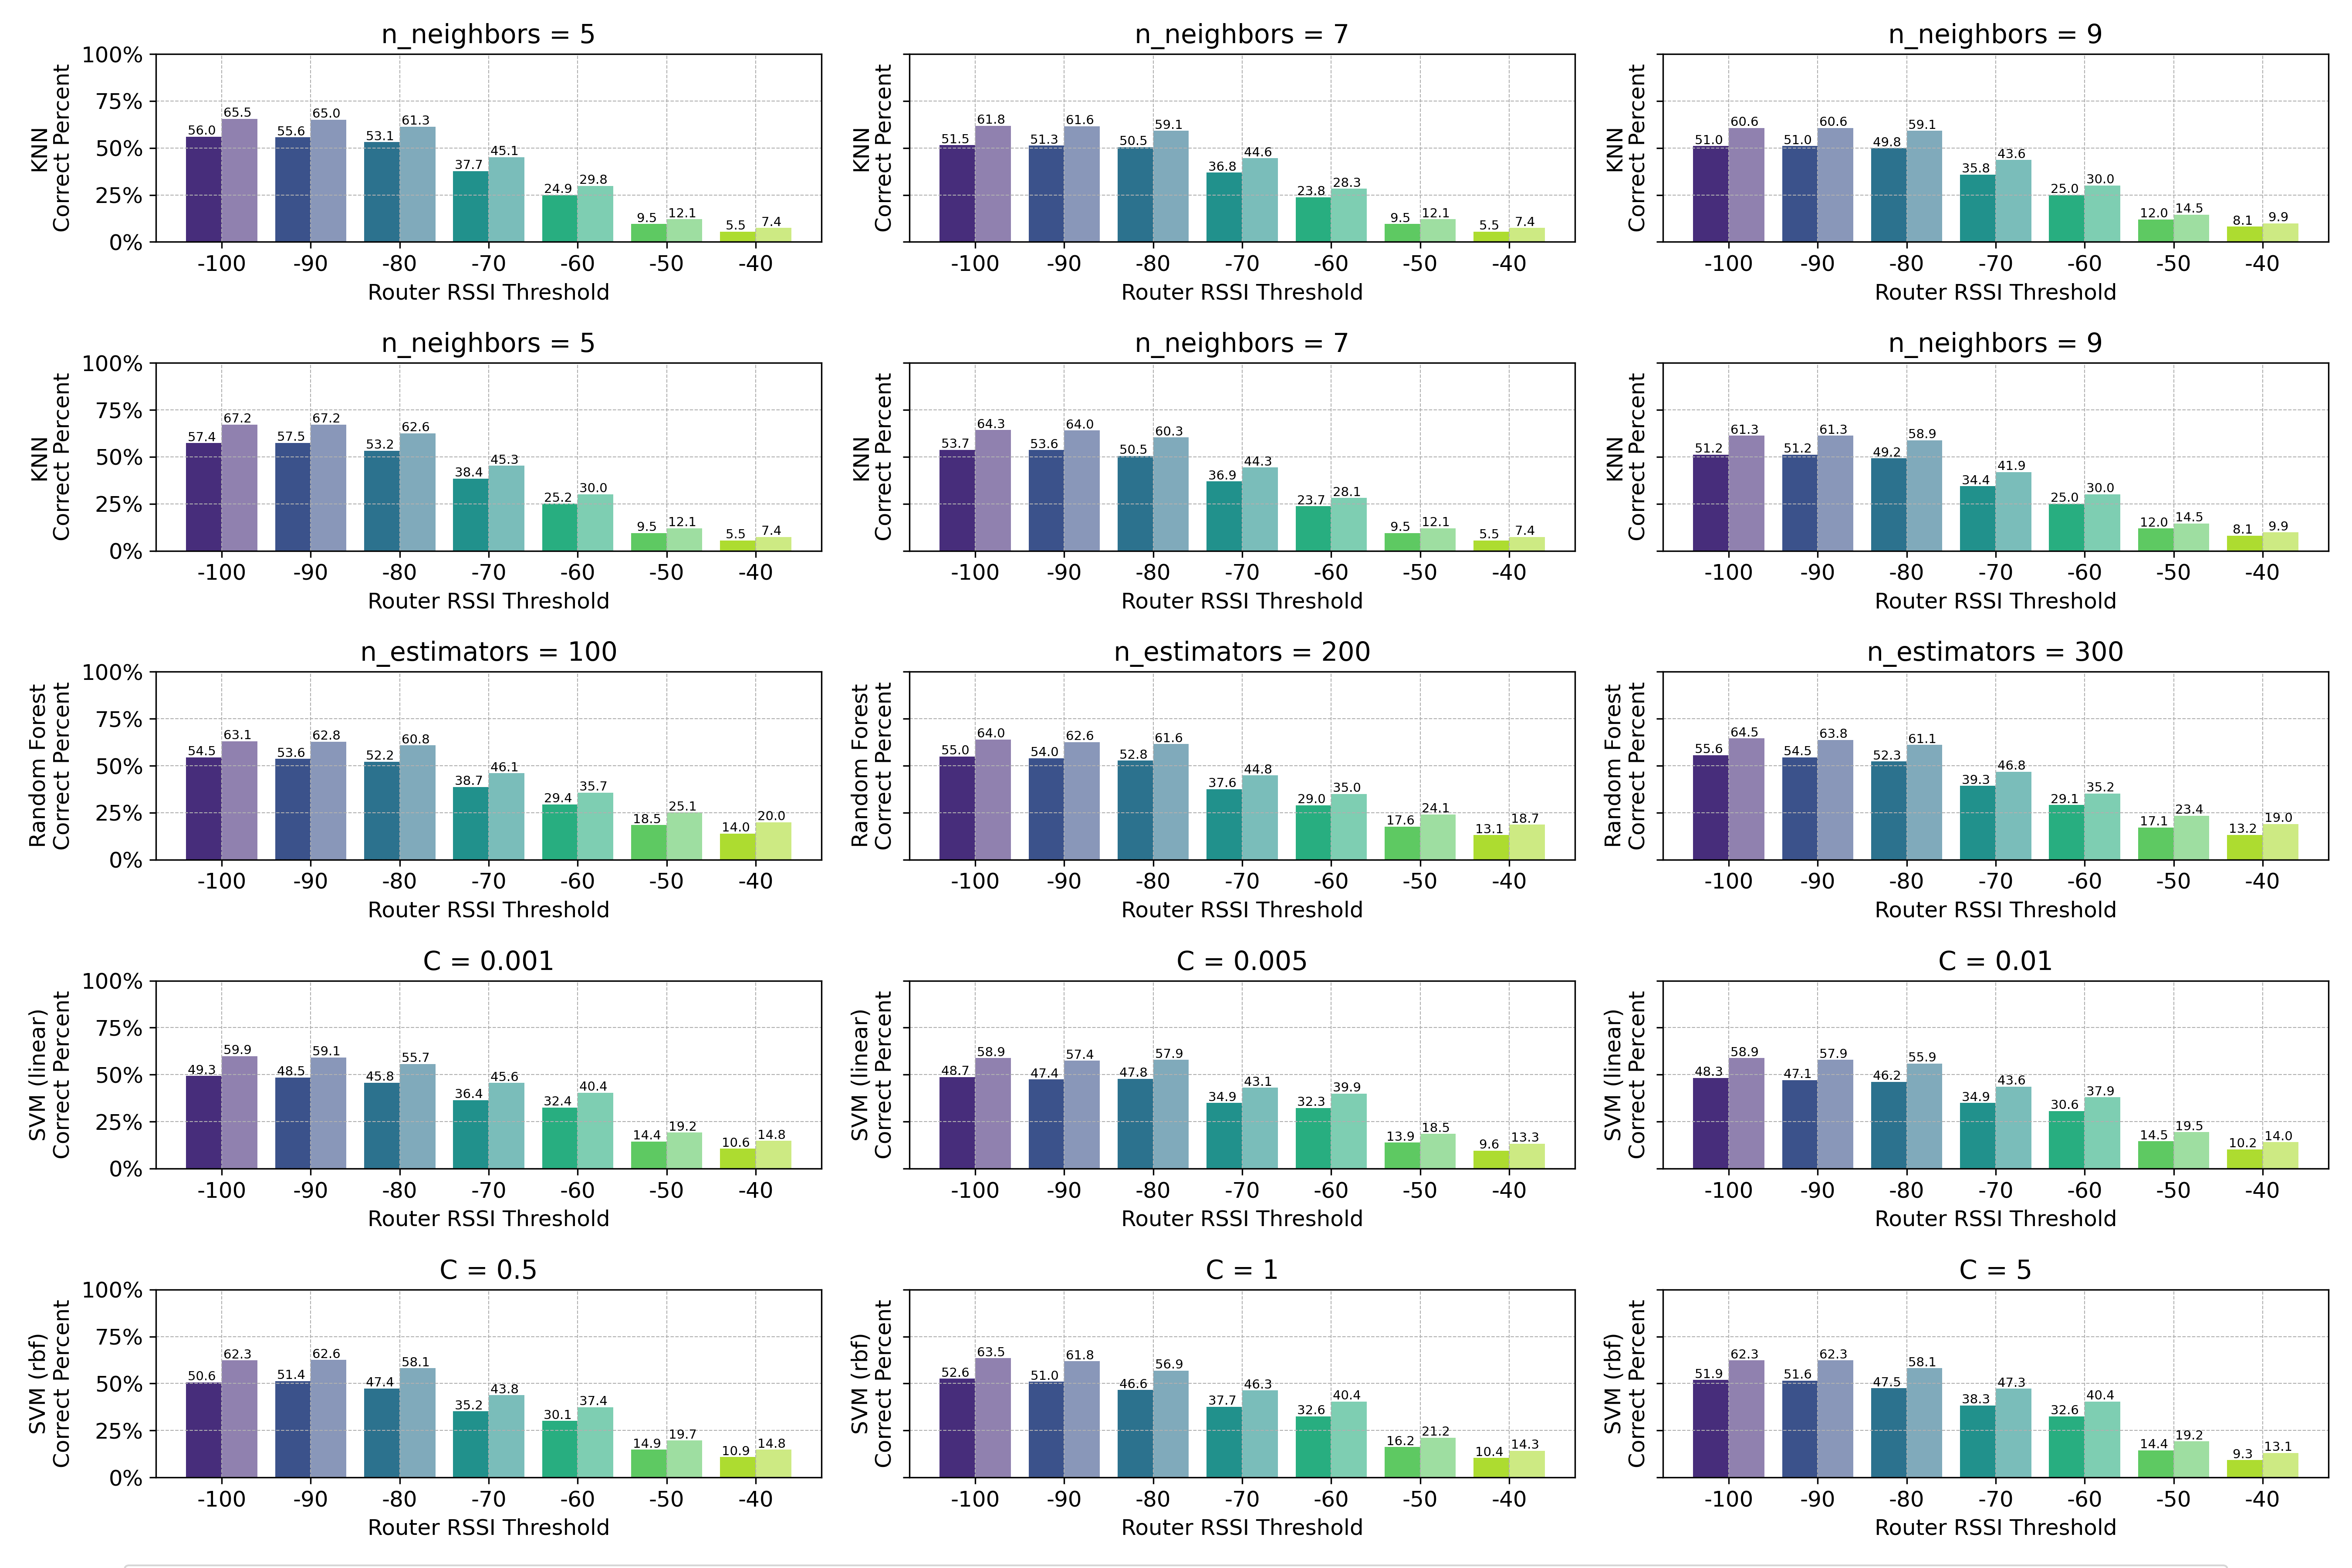
\includegraphics[width=0.8\textwidth]{images/6_router_rssi_threshold_01.png}
    \caption{Router Rssi Threshold}
    \label{fig:6_router_rssi_threshold_01}
\end{figure}

\subsection{Skalierung von RSSI-Werten}

\subsubsection{Formeln}

Quelle XX: Comprehensive analysis of distance and similarity measures for Wi-Fi fingerprinting indoor positioning systems

Die Idee hinter der Werteskalierung stammt aus der Quelle XX und basiert auf der Erkenntnis, dass die RSSI-Werte nicht linear verteilt sind. Durch eine geeignete Skalierung kann der Zusammenhang zwischen Entfernung und RSSI-Wert besser abgebildet werden. In der vorliegenden Arbeit wurden drei Skalierungsmethoden aus der Quelle XX implementiert und verglichen.

Grundlage jeder Skalierung ist die positive Darstellung der Werte. Hierfür wird von allen RSSI-Werten aus den Trainings- und Testdaten der niedrigste gemessene RSSI-Wert minus 1 subtrahiert:

\begin{equation}
    \text{Positiv}_i(x) = \text{RSS}_i - \text{min}
    \label{eq:positive_values_representation}
\end{equation}

wobei \(\text{min}\) der niedrigste RSS-Wert minus 1 ist, der alle Fingerabdrücke und WAPs in der Datenbank berücksichtigt.

Anschließend werden die Werte auf drei verschiedene Arten skaliert: linear, exponentiell und potenziert.

**Lineare Normalisierung:**

Die linear normalisierten Werte werden berechnet als:

\begin{equation}
    \text{NullBisEinsNormalisiert}_i(x) = \frac{\text{Positiv}_i(x)}{-\text{min}}
    \label{eq:linear_normalized_values}
\end{equation}

**Exponentielle Skalierung:**

Die exponentiell skalierten Werte werden berechnet unter Verwendung von \(\alpha = 24\):

\begin{equation}
    \text{Exponentiell}_i(x) = \frac{\exp\left(\frac{\text{Positiv}_i(x)}{\alpha}\right)}{\exp\left(\frac{-\text{min}}{\alpha}\right)}
    \label{eq:exponential_representation}
\end{equation}

**Potenzierte Skalierung:**

Die potenzierten Werte werden berechnet unter Verwendung von \(\beta = e\):

\begin{equation}
    \text{Potenz}_i(x) = \left(\frac{\text{Positiv}_i(x)}{-\text{min}}\right)^{\beta}
    \label{eq:powered_representation}
\end{equation}

In Abbildung \ref{fig:value_scaling_strategies_ignore_10} sind die verschiedenen Skalierungsmethoden dargestellt.

\begin{figure}[H]
    \centering
    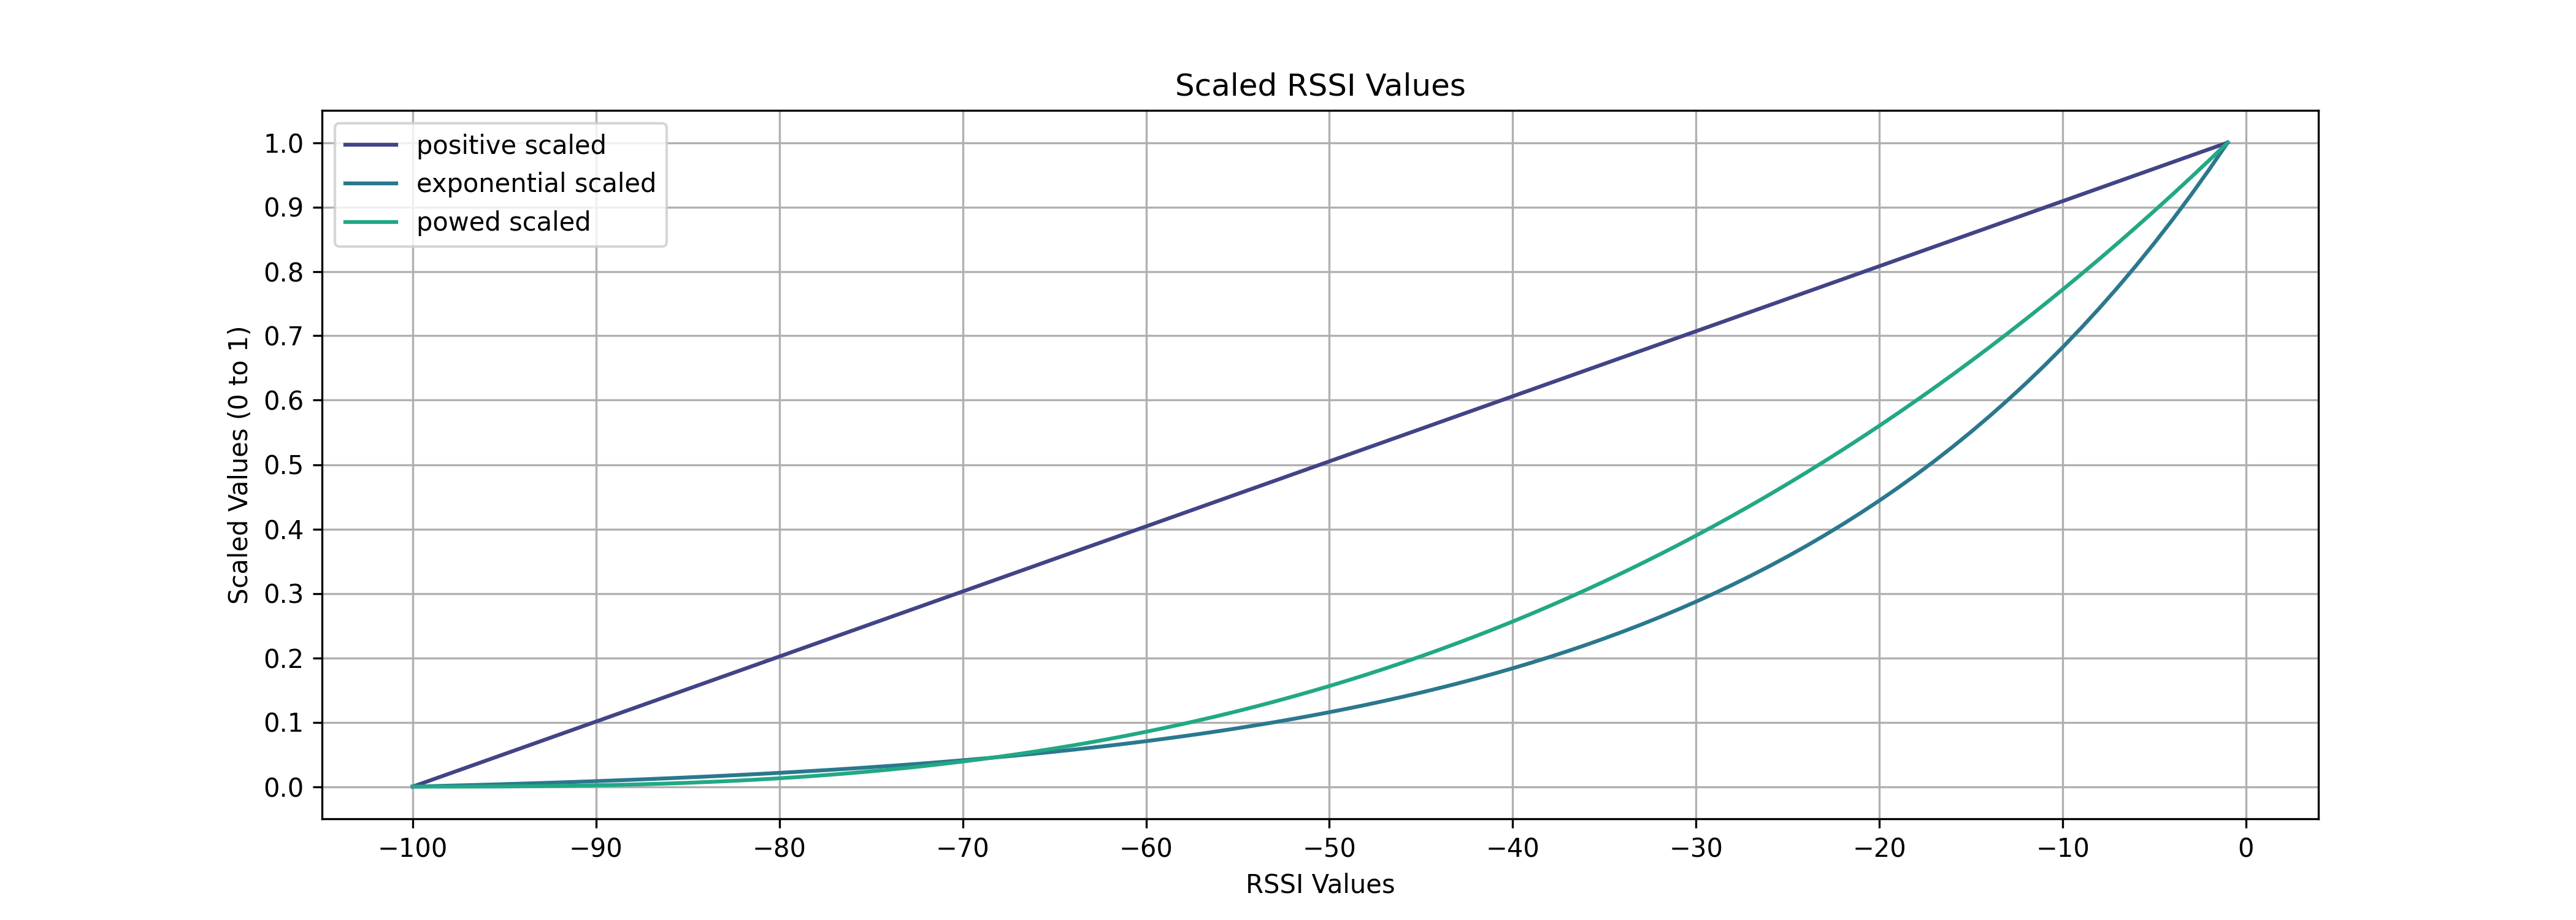
\includegraphics[width=0.8\textwidth]{images/value_scaling_strategies_ignore_10.png}
    \caption{Value Scaling Strategies}
    \label{fig:value_scaling_strategies_ignore_10}
\end{figure}


\subsubsection{Nochmal KNN Uniform vs. Distance}

Durch die Skalierung könnte es sein, dass die ursprüngliche Wahl der distance KNN Methode nicht mehr die beste ist. Aus diesem Grund wird vor der Untersuchung der Skalierungsmethoden nochmal der Vergleich zwischen distance und uniform durchgeführt in Zusammenhang mit den Skalierungsmethoden.

\begin{figure}[H]
    \centering
    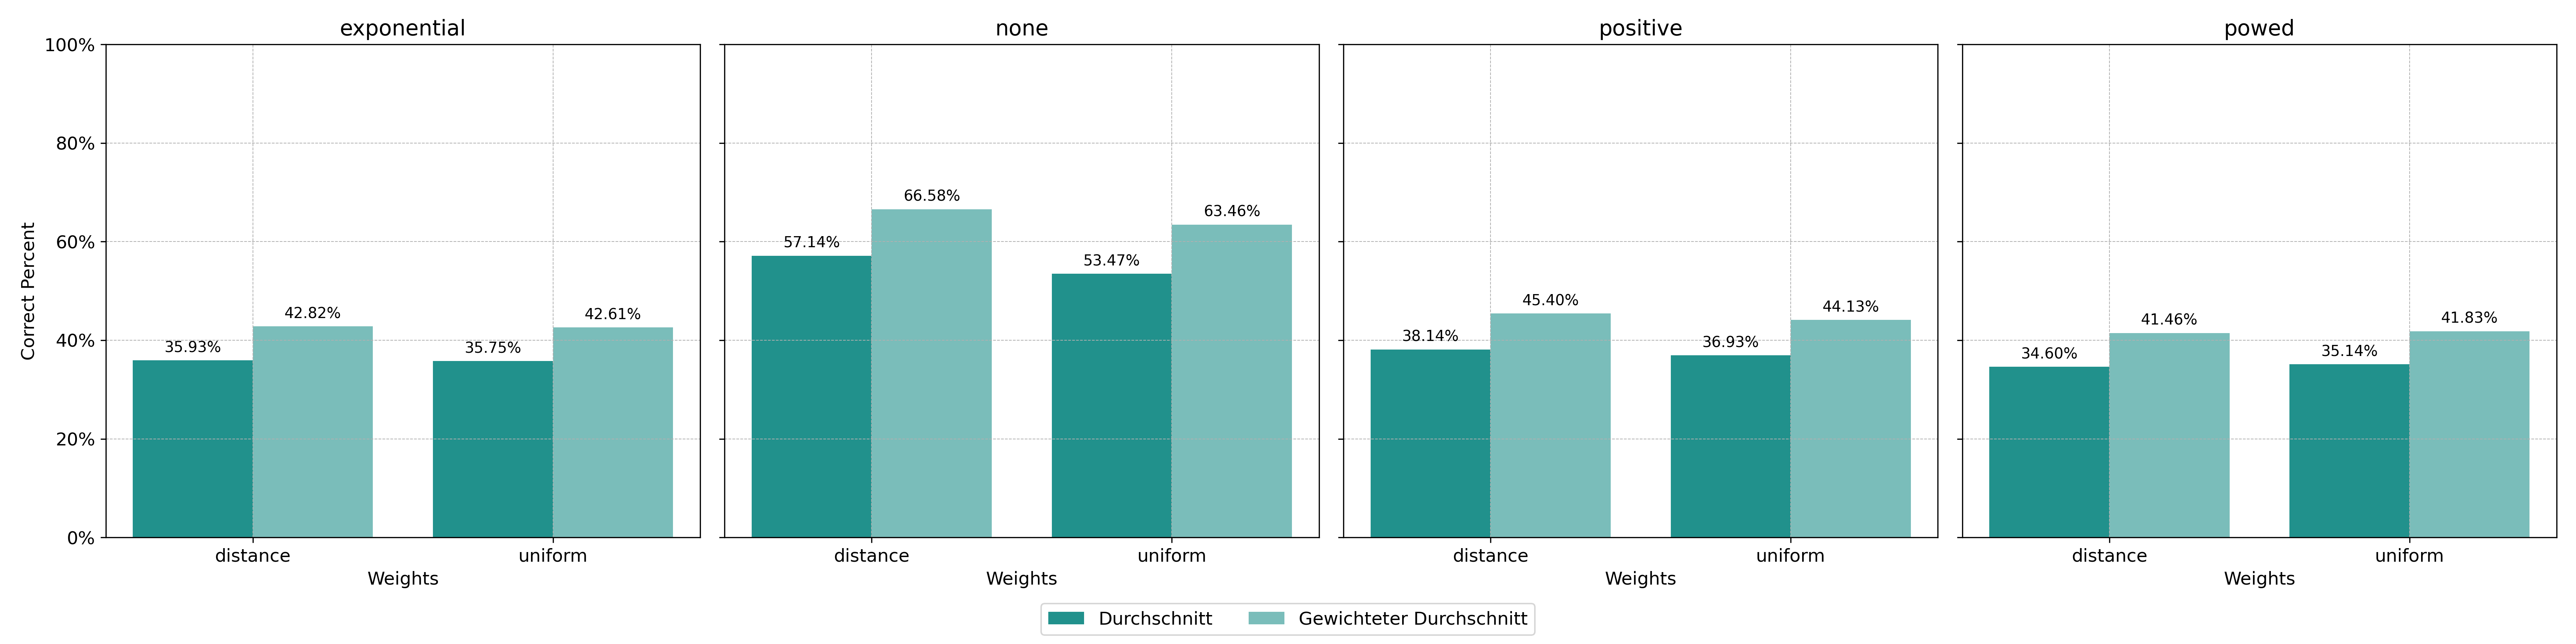
\includegraphics[width=0.8\textwidth]{images/7_value_scaling_strategy_knn_distance_02.png}
    \caption{KNN Uniform vs. Distance im Durchschnitt}
    \label{fig:7_value_scaling_strategy_knn_distance_02}
\end{figure}

\begin{figure}[H]
    \centering
    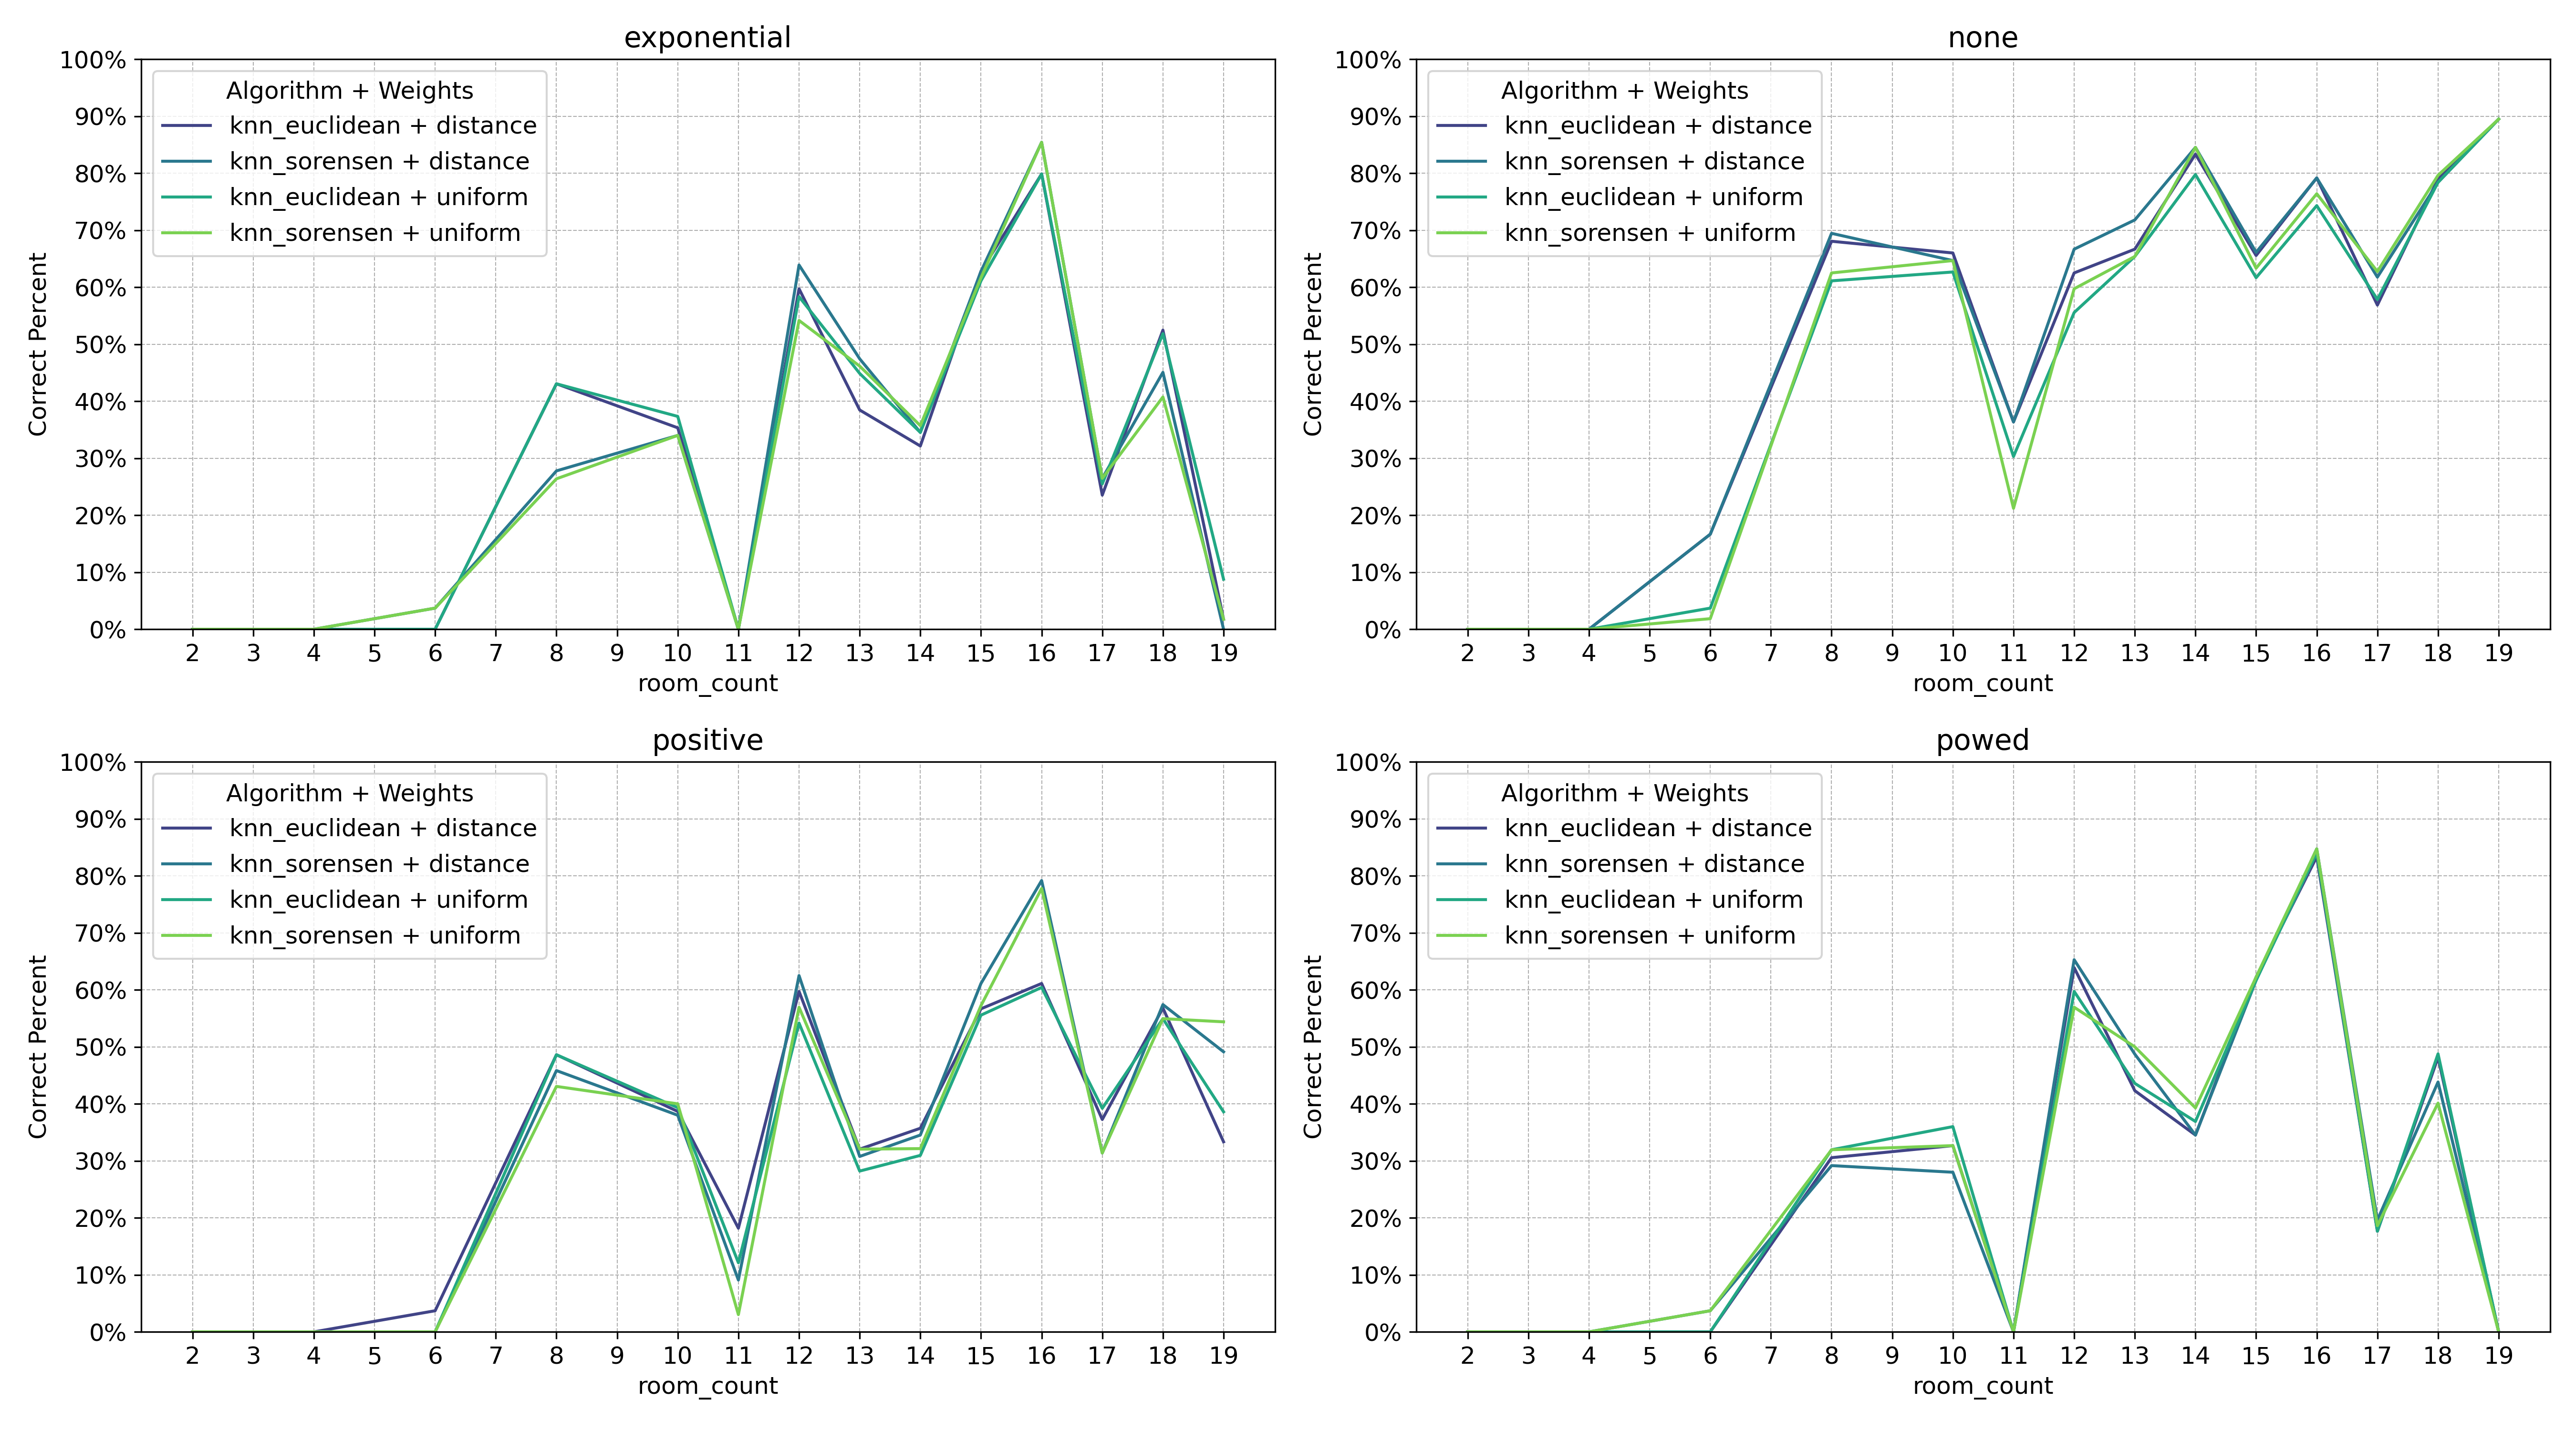
\includegraphics[width=0.8\textwidth]{images/7_value_scaling_strategy_knn_distance_03.png}
    \caption{KNN Uniform vs. Distance pro Raum}
    \label{fig:7_value_scaling_strategy_knn_distance_03}
\end{figure}

Wie zu erkenne ist, ist distance weiterhin besser als uniform. Aus diesem Grund wird weiterhin die distance weights Methode verwendet.

In Abbildung \ref{fig:7_value_scaling_strategy_02} folgendes zu erkennen:

\begin{itemize}
    \item In den meisten fällen sehr ähnlicher Verlauf --> Es gibt Unterschiede bei den Skalierungsmethoden, aber bei den Skalierungsmethoden sind die Ergebnisse bei euclidean/sorensen und distance/uniform sehr ähnlich
    \item Bei exponential: distance ist besser als uniform bei wenigen Messungen pro Raum
    \item Bei none: distanz ist etwas besser als uniform bei wenigeren Messungen. Abstand nimmt aber ab mit der Anzahl an Messungen
    \item Bei exponential, powed (und auch leicht bei positive): Nimmt die Genauigkeit mit zunehmender Anzahl an Messungen wieder ab. Bisher hatten die Räume mit den meisten Messungen immer die größten Genauigkeiten. In diesem Fall haben die Räume mit 16 Messungen die höchste Genauigkeit und danach nimmt es wieder ab. Bei exponential und powed ist die Genauzigkeit bei n = 19 sogar wieder bei fast allen Kombinationen aus distance und weights bei 0\%!
\end{itemize}

\begin{figure}[H]
    \centering
    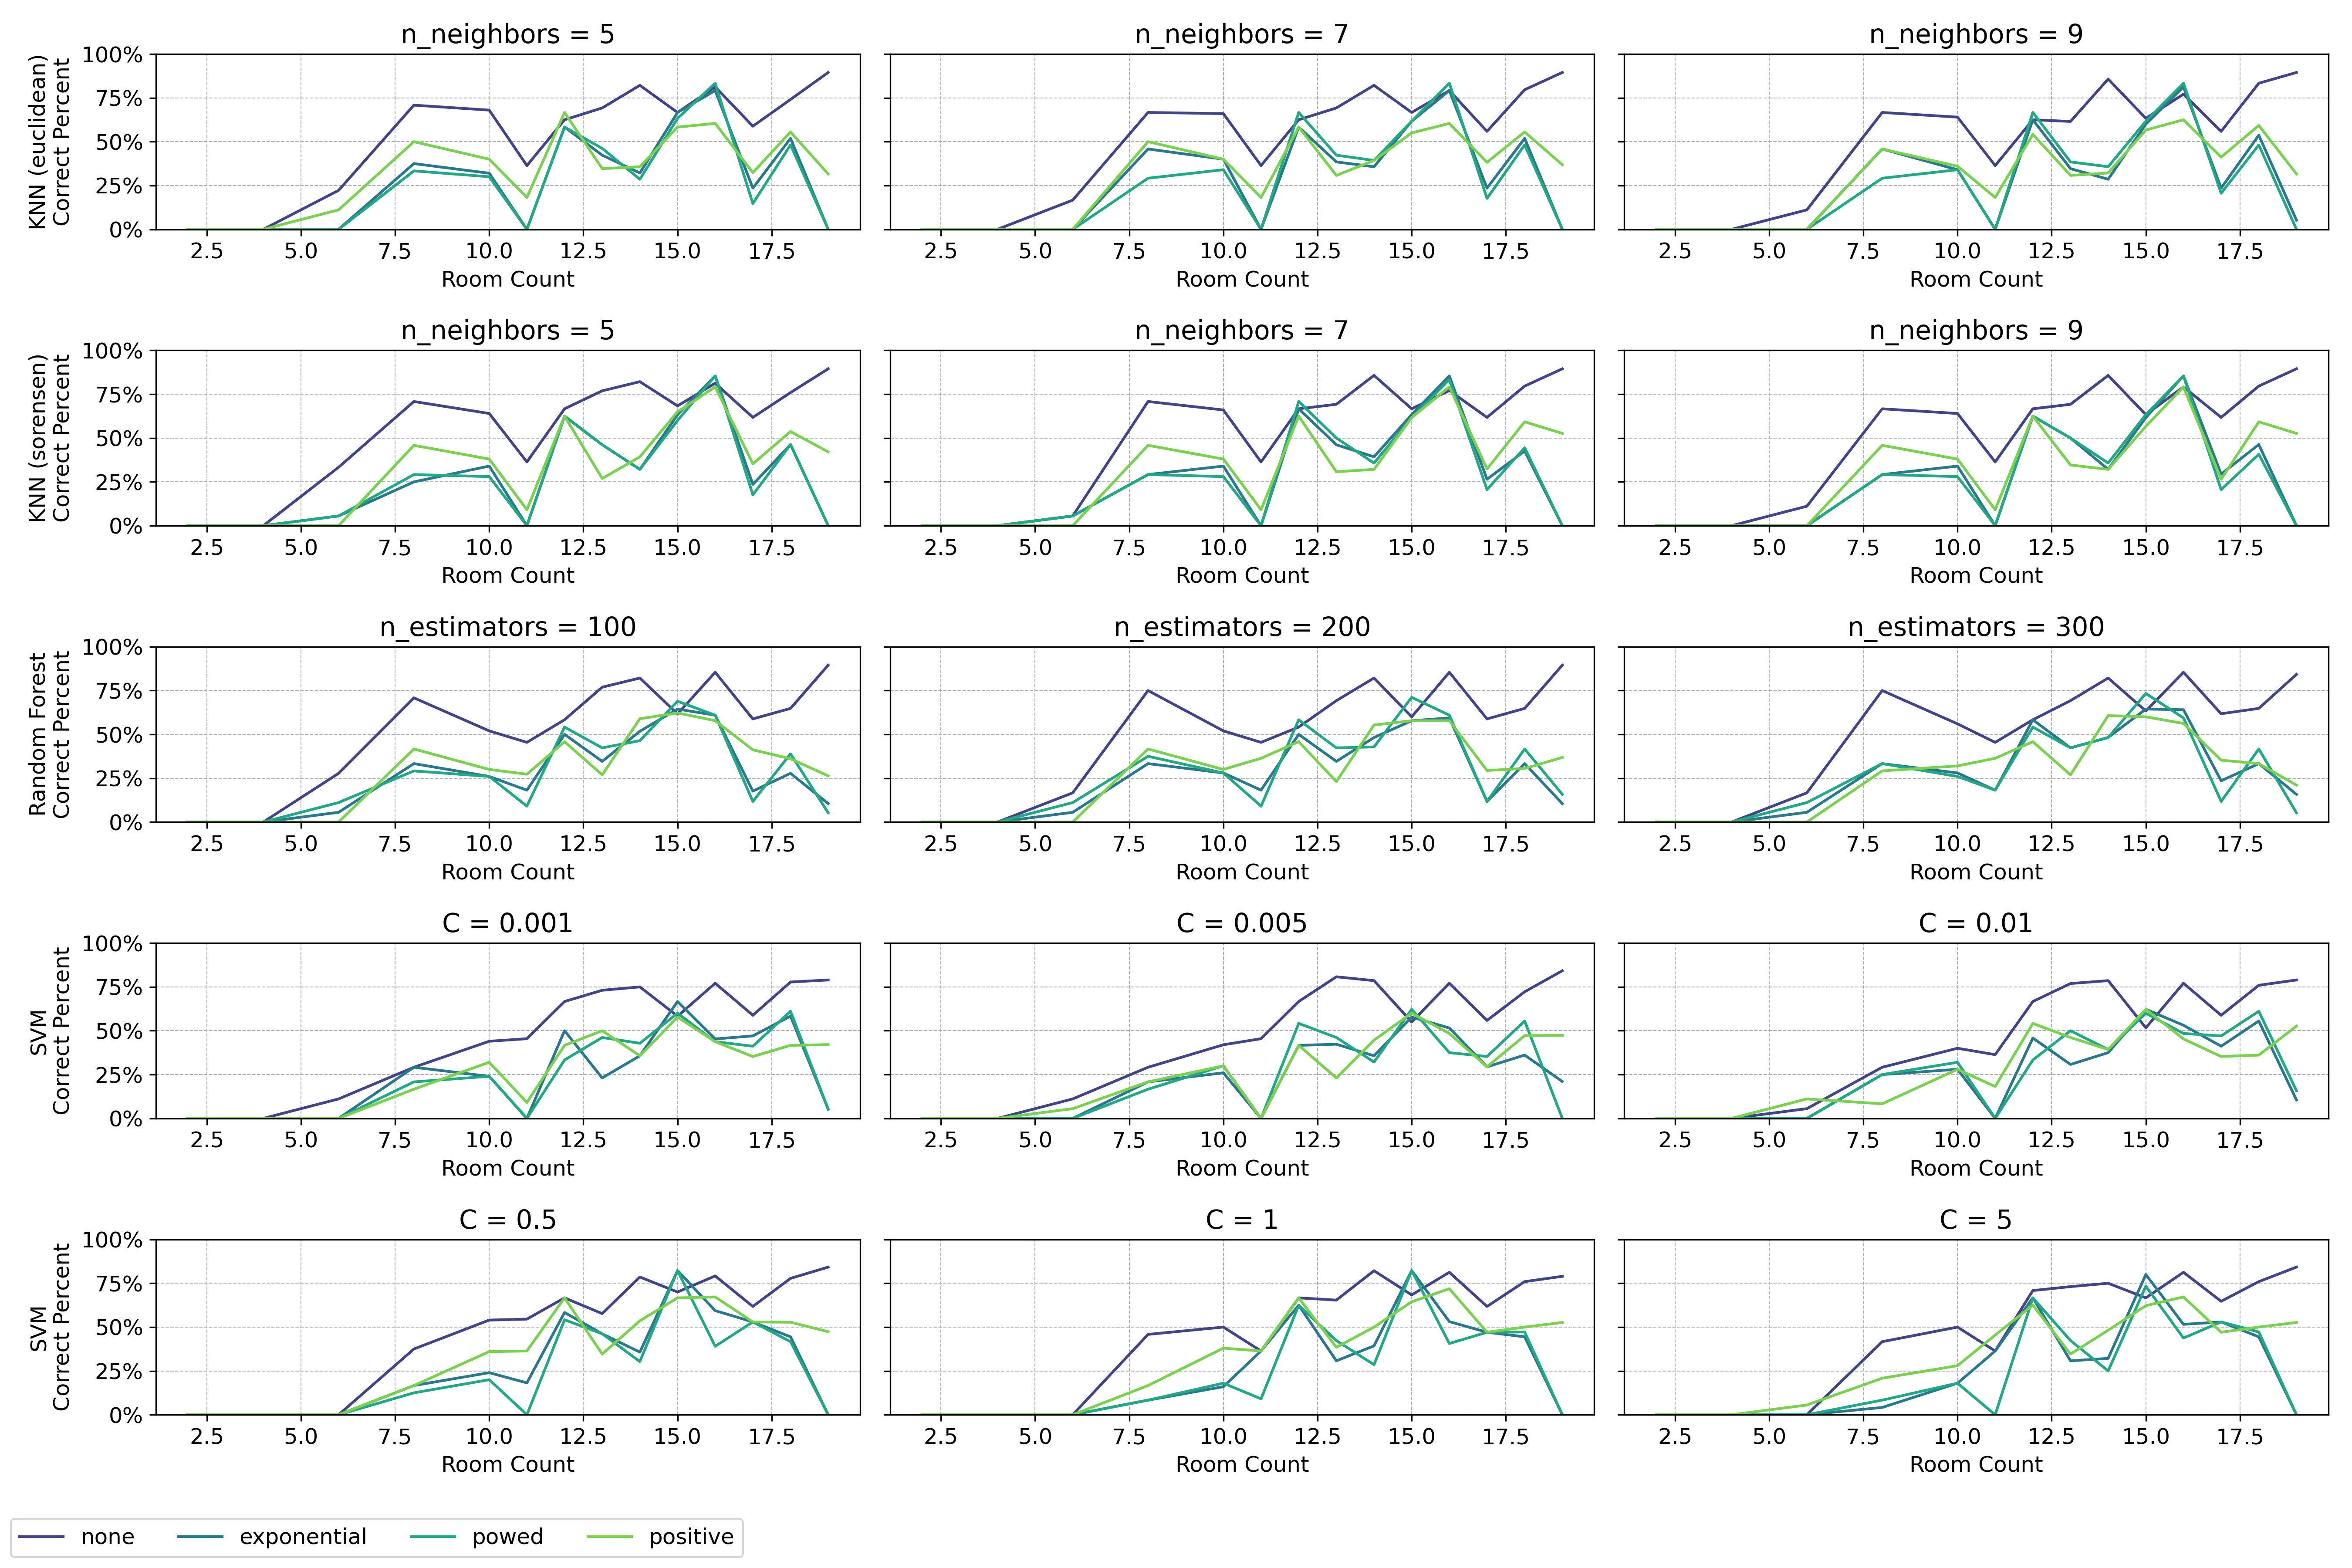
\includegraphics[width=0.8\textwidth]{images/7_value_scaling_strategy_02.png}
    \caption{Skalierungsstrategeien nach Algorithmus und Parameter pro Anzahl Messungen pro Raum}
    \label{fig:7_value_scaling_strategy_02}
\end{figure}

\section{Erweiterte Untersuchungen}

\subsection{Einfluss der Anzahl der Fingerprints auf die Genauigkeit}

In der folgenden Untersuchung wird im Detail untersucht, wie sich die Anzahl an Messungen auf die Genauigkeit der Ergebnisse wiederspiegelt. Dafür werden in diesem Fall die Trainingsdaten erweitern, sodass in 4 nahegelgenen Räumen je 20 Messungen gemacht wurden. Aufgrundlage dieser Messungen wird nun überprüft, wie sich der bis jetzt beste Algorithmus schlägt.

TODO: Lineplot mit den Ergebnissen (So wie die Heatmap, aber halt nur eine Achse)

\subsection{Verbesserung der Vorhersagegenauigkeit durch Fingerprints außerhalb der Räume}

Für eine noch bessere Genauigkeit wurde jetzt untersucht, wie sich die Genauigkeit verbessert, wenn zusätzlich zu den Fingerabdrücken innerhalb der Räume auch Fingerabdrücke außerhalb der Räume verwendet werden und somit auch vorhergesagt werden kann, dass kein korrekter Raum ermittelt werden konnte. Das ist sinnvoll, da in diesen Fällen die ESP32 keine Messdaten für falsche Räume veröffentlichen bzw. in weniger Fällen flasche Ergebnisse veröffentlichen kann.

\begin{figure}[H]
    \centering
    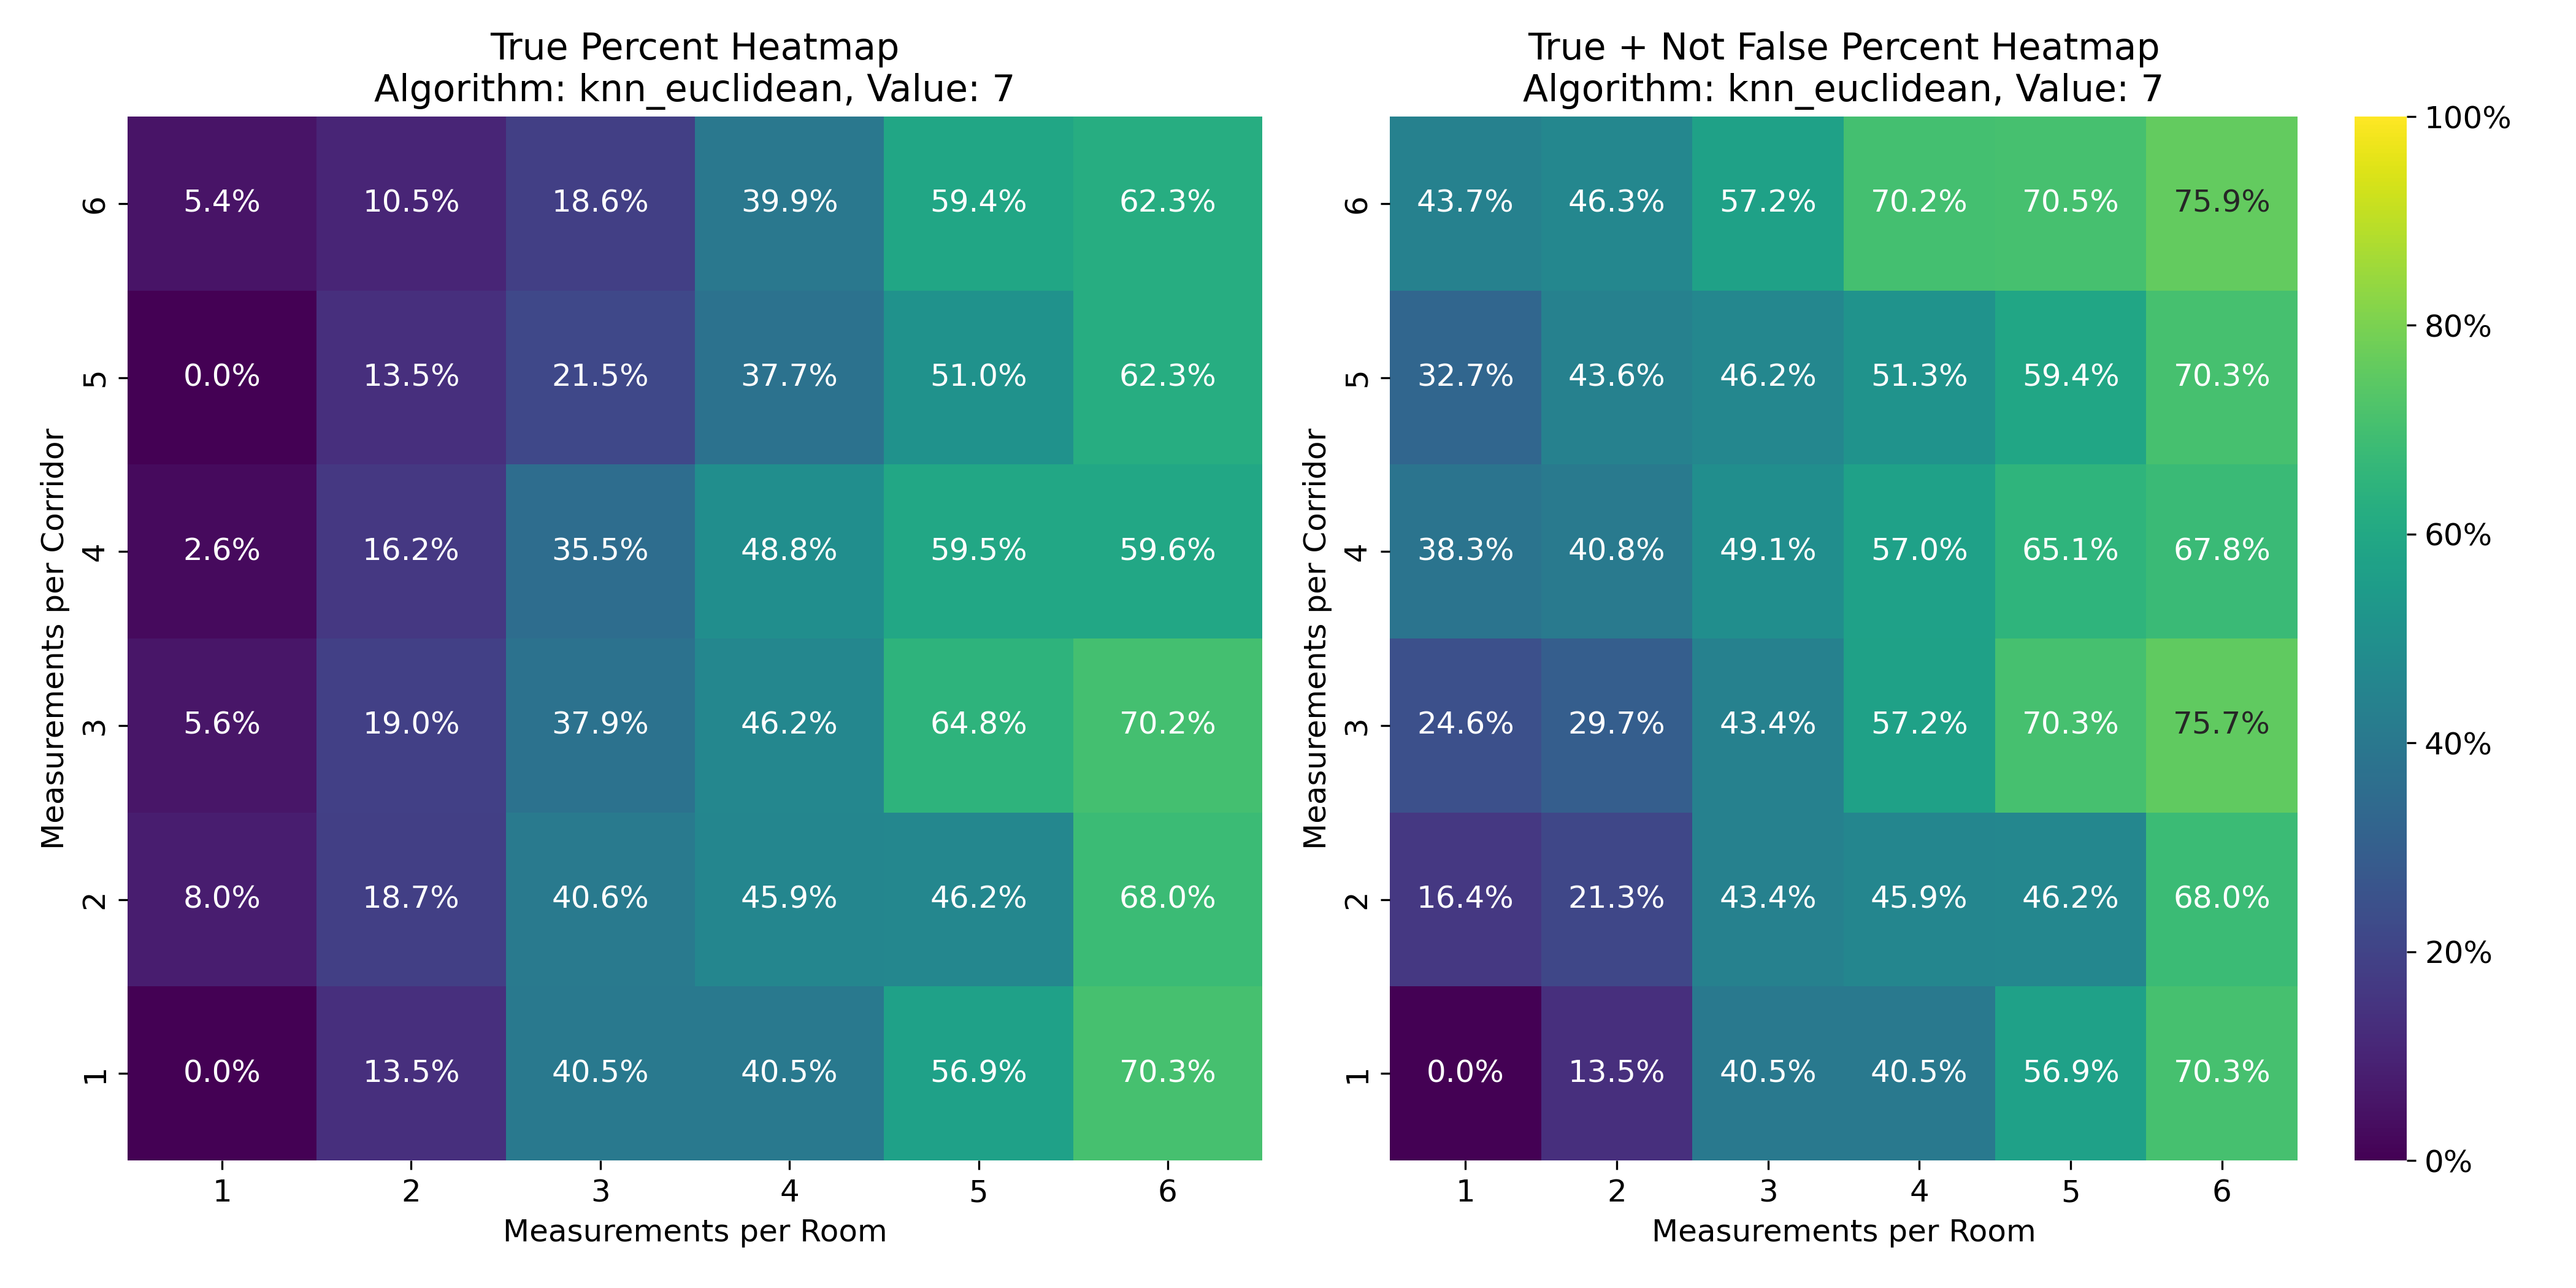
\includegraphics[width=0.8\textwidth]{images/8_test_corrdior_01.png}
    \caption{Ergebnisse unter Betrachtung von Messungen außerhalb der Räume}
    \label{fig:8_test_corrdior_01}
\end{figure}

\chapter{Fazit und Ausblick}
\section{Zusammenfassung der Ergebnisse}
\section{Diskussion der Ergebnisse}
\section{Ausblick auf zukünftige Arbeiten}




% Appendices
\appendix
\clearpage
\pagenumbering{Roman}

% Including appendices
\chapter{Ergänzende Informationen}
\label{app:informationen}

\section{Zusätzliche Daten}
\lipsum[3]

% \input{appendices/python_code}

% Bibliography without numbering
\printbibliography

\clearpage


% Print glossary and acronym list
\begin{minipage}{\textwidth}
    \printglossary[type=main,title=Glossar]
    \vspace{7em} % optional space between glossary and acronym list
    \printglossary[type=\acronymtype,title=Abkürzungsverzeichnis]
\end{minipage}



% Affidavit
\clearpage
\chapter*{Eidesstattliche Versicherung}
Hiermit versichere ich, dass ich die vorliegende Arbeit selbstständig und ohne unzulässige Hilfe Dritter angefertigt habe. Sämtliche Stellen, die wörtlich oder sinngemäß aus veröffentlichten oder unveröffentlichten Quellen entnommen sind, habe ich als solche kenntlich gemacht. Die Arbeit hat in gleicher oder ähnlicher Form noch keiner Prüfungsbehörde vorgelegen.

\vspace{3cm}

\begin{table}[h]
    \begin{tabularx}{\textwidth}{p{5cm}X p{5cm}}
        Berlin, \today           &  &                                 \\\cline{1-1} \cline{3-3}
        \vspace{0.1em}Ort, Datum &  & \vspace{0.1em}Friedrich Völkers
    \end{tabularx}
\end{table}


% Signature
\vspace{-3.3cm}
\begin{center}
    \hspace{11cm}
\includegraphics[width=0.25\textwidth]{images/signature.png} % Adjust position
\end{center}

\end{document}
